% !TEX program = xelatex
\documentclass[UTF8]{ctexart}

%基本配置
\RequirePackage{inputenc}
\RequirePackage{fontspec}
\RequirePackage{xeCJK}

%数学字体
\RequirePackage{amsmath}
\RequirePackage{amssymb}
\RequirePackage{bm}

%物理单位
\RequirePackage{siunitx}

%物理符号
\RequirePackage{physics}

%绘图
\RequirePackage{tikz}
\RequirePackage{circuitikz}     %绘制电路图
\RequirePackage{tkz-euclide}    %绘制平面几何
\usetkzobj{all}
\usetikzlibrary{angles}
\usetikzlibrary{calc}
\usetikzlibrary{arrows.meta}

%排版
\RequirePackage[hidelinks]{hyperref}    %添加目录超链接
\RequirePackage{titlesec}               %修改标题样式
\RequirePackage{subfigure}              %添加子图片

\setmainfont{Times New Roman}

\setCJKmainfont{等线}
\setCJKsansfont{等线}
\setCJKmonofont{等线}

%粗体向量
\newcommand*{\veb}[1]{\vb*{#1}}

%导数符号
\newcommand*{\dif}{\mathop{}\!\mathrm{d}}

%罗马数字
\newcommand{\rnum}[1]{\uppercase\expandafter{\romannumeral #1\relax}}

%字体大小
\newcommand{\sizeN}[1]{{\normalsize #1}}

\newcommand{\sizeLA}[1]{{\large #1}}
\newcommand{\sizeLB}[1]{{\Large #1}}
\newcommand{\sizeLC}[1]{{\LARGE #1}}
\newcommand{\sizeLD}[1]{{\huge #1}}
\newcommand{\sizeLE}[1]{{\Huge #1}}

\newcommand{\sizeSA}[1]{{\small #1}}
\newcommand{\sizeSB}[1]{{\footnotesize #1}}
\newcommand{\sizeSC}[1]{{\scriptsize #1}}
\newcommand{\sizeSD}[1]{{\tiny #1}}

\RequirePackage{geometry}
\geometry
{
    left=1.25in,
    right=1.25in,
    top=1in,
    bottom=1in
}

\title{大学物理笔记}
\author{李宇轩}
\date{2020.07.01}

\begin{document}

\definecolor{LightGray}{rgb}{0.95,0.95,0.95}
\definecolor{MediumGray}{rgb}{0.7,0.7,0.7}

%绘制标题
\maketitle

\newpage

%绘制目录
\tableofcontents

%正文基本设置
\setlength{\parindent}{0pt}
\titleformat{\part}{\centering\bfseries\Huge}{第~\chinese{part}~部分}{40pt}{}

\newpage

\part{力}

\newpage

\section{质点的运动}
    质点是一种理想模型,只具有质量,没有大小,没有形状。\\[3mm]
    例如当研究地球的公转时,可以将地球视作质点。\\[3mm]
    例如当研究地球的自转时,不能将地球视作质点。

\subsection{运动的线量描述}
    运动的线量描述可以用于研究质点在空间直角坐标系的运动。\\[3mm]
    运动的线量描述包含:
    \begin{table}[h]
        \begin{center}
            \begin{tabular}{p{60pt}|p{60 pt}|p{60 pt}}
                \hline
                位矢&$\veb{r}$&\si{m}\\ \hline
                速度&$\veb{v}$&\si{m/s}\\ \hline
                加速度&$\veb{a}$&\si{m/s^2}\\ \hline
            \end{tabular}
            \caption{运动的线量描述}
        \end{center}
    \end{table}\vspace{-25pt}

\subsubsection{位矢}
    位矢描述了物体的位置,其变化量称为位移,是一个矢量,通常用符号$\veb{r}$表示,单位是\si{m}。\\[3mm]
    位矢可以表示为:
    \begin{large}
        \begin{equation*}
            \veb{r}=x\veb{i}+y\veb{j}+z\veb{k}\vspace{-5pt}
        \end{equation*}
    \end{large}\\
    位矢的大小可以表示为:
    \begin{large}
        \begin{equation*}
            r=|\veb{r}|=\sqrt{x^2+y^2+z^2}\vspace{-5pt}
        \end{equation*}
    \end{large}\\
    其中$x,y,z$代表三个坐标轴上的位矢分量,而$\veb{i},\veb{j},\veb{k}$则代表三个坐标轴上的单位矢量。\\[6mm]
    三维空间中的运动学方程:
    \begin{large}
        \begin{equation*}
            x=x(t)~~~~~~~~y=y(t)~~~~~~~~z=z(t)\vspace{-5pt}
        \end{equation*}
    \end{large}\\
    二维空间中的运动学方程:
    \begin{large}
        \begin{equation*}
            x=x(t)~~~~~~~~y=y(t)\vspace{-5pt}
        \end{equation*}
    \end{large}\\
    运动学方程可以视作位矢关于时间的参数方程。\\[3mm]
    运动学方程中消去时间即可得到轨迹方程。

\newpage

\subsubsection{速度}
    速度衡量了位矢的变化快慢,是一个矢量,通常用符号$\veb{v}$表示。单位是\si{m/s}。\\[3mm]
    平均速度的定义:
    \begin{large}
        \begin{equation*}
            \bar{\veb{v}}=\frac{\Delta \veb{r}}{\Delta t}
        \end{equation*}
    \end{large}\\
    瞬时速度的定义:
    \begin{large}
        \begin{equation*}
            \veb{v}=\lim_{\Delta t\rightarrow 0}\frac{\Delta \veb{r}}{\Delta t}=\frac{\dif\veb{r}}{\dif t}
        \end{equation*}
    \end{large}\\
    速度通常指的就是瞬时速度。\\[3mm]
    速度定义为平均速度在时间趋近零时的极限,速度是位矢关于时间的一阶导数。\\[3mm]
    速度$\veb{v}$的方向和位矢的瞬时变化量$\dif\veb{r}$的方向相同,但与位矢$\veb{r}$的方向无关。\\[6mm]
    通过以下推导:
    \setcounter{equation}{0}
    \begin{align}
        \veb{v}
        &=\frac{\dif\veb{r}}{\dif t}\\[3mm]
        &=\frac{\dif}{\dif t}\left(x\veb{i}+y\veb{j}+z\veb{k}\right)\\[3mm]
        &=\frac{\dif x}{\dif t}\veb{i}+\frac{\dif y}{\dif t}\veb{j}+\frac{\dif z}{\dif t}\veb{k}\\[3mm]
        &=v_x\veb{i}+v_y\veb{j}+v_z\veb{k}
    \end{align}\\
    速度可以表示为:
    \begin{large}
        \begin{equation*}
            \veb{v}=v_x\veb{i}+v_y\veb{j}+v_z\veb{k}
        \end{equation*}
    \end{large}\\
    速度的大小可以表示为:
    \begin{large}
        \begin{equation*}
            v=|\veb{v}|=\sqrt{v_x^2+v_y^2+v_z^2}
        \end{equation*}
    \end{large}\\
    其中$v_x,v_y,v_z$代表三个坐标轴上的速度分量,而$\veb{i},\veb{j},\veb{k}$则代表三个坐标轴上的单位矢量。\\[6mm]
    因为速度是位矢关于时间的导数,所以位矢是速度关于时间的积分:\vspace{5pt}
    \begin{large}
        \begin{equation*}
            \veb{r}=\int \veb{v}\cdot\dif t
        \end{equation*}
    \end{large}\\
    通过该公式,可以在已知速度的情况下求解位矢。

\newpage

\subsubsection{加速度}
    加速度衡量了速度的变化快慢,是一个矢量,通常用符号$\veb{a}$表示。单位是\si{m/s^2}。\\[3mm]
    平均加速度的定义:
    \begin{large}
        \begin{equation*}
            \bar{\veb{a}}=\frac{\Delta \veb{v}}{\Delta t}
        \end{equation*}
    \end{large}\\
    瞬间加速度的定义:
    \begin{large}
        \begin{equation*}
            \veb{a}=\lim_{\Delta t\rightarrow 0}\frac{\Delta \veb{v}}{\Delta t}=\frac{\dif\veb{v}}{\dif t}
        \end{equation*}
    \end{large}\\
    加速度通常指的就是瞬时加速度。\\[3mm]
    加速度定义为平均加速度在时间趋近于零时的极限,加速度是速度关于时间的一阶导数。\\[3mm]
    加速度$\veb{a}$的方向和速度的瞬时变化量$\dif\veb{v}$的方向相同,但与速度$\veb{v}$的方向无关。\\[6mm]
    通过以下推导:
    \setcounter{equation}{0}
    \begin{align}
        \veb{a}
        &=\frac{\dif\veb{v}}{\dif t}\\[3mm]
        &=\frac{\dif}{\dif t}\left(v_x\veb{i}+v_y\veb{j}+v_z\veb{k}\right)\\[3mm]
        &=\frac{\dif v_x}{\dif t}\veb{i}+\frac{\dif v_y}{\dif t}\veb{j}+\frac{\dif v_z}{\dif t}\veb{k}\\[3mm]
        &=a_x\veb{i}+a_y\veb{j}+a_z\veb{k}
    \end{align}\\
    加速度可以表示为:
    \begin{large}
        \begin{equation*}
            \veb{a}=a_x\veb{i}+a_y\veb{j}+a_z\veb{k}
        \end{equation*}
    \end{large}\\
    加速度的大小可以表示为:
    \begin{large}
        \begin{equation*}
            a=|\veb{a}|=\sqrt{a_x^2+a_y^2+a_z^2}
        \end{equation*}
    \end{large}\\
    其中$a_x,a_y,a_z$代表三个坐标轴上的加速度分量,而$\veb{i},\veb{j},\veb{k}$则代表三个坐标轴上的单位矢量。\\[6mm]
    因为加速度是速度关于时间的导数,所以速度是加速度关于时间的积分:\vspace{5pt}
    \begin{large}
        \begin{equation*}
            \veb{v}=\int \veb{a}\cdot\dif t
        \end{equation*}
    \end{large}\\
    通过该公式,可以在已知加速度的情况下求解速度。

\newpage

\subsection{直线运动}
    质点的运动轨迹是直线的运动,称为直线运动。

\subsubsection{匀变速直线运动}
    \setcounter{equation}{0}
    在匀变速直线运动中,加速度$a$是一个常数。\\[3mm]
    通过对加速度的积分,可以得到速度:
    \begin{align}
        v
        &=\int a\cdot\dif t~~~~~~~~~~~~~~~~~~~~\\[3mm]
        &=a\cdot t+v_0
    \end{align}\\
    通过对速度的积分,可以得到位矢:
    \begin{align}
        ~~r
        &=\int v\cdot\dif t\\[3mm]
        &=\int (a\cdot t+v_0)\cdot\dif t\\[3mm]
        &=\frac{1}{2}\cdot a\cdot t^2+v_0\cdot t+r_0
    \end{align}\\
    匀变速直线运动中物体的速度:
    \begin{large}
        \begin{equation*}
            v=a\cdot t+v_0            
        \end{equation*}
    \end{large}\\
    匀变速直线运动中物体的位移:
    \begin{large}
        \begin{equation*}
            r=\frac{1}{2}\cdot a\cdot t^2+v_0\cdot t+r_0
        \end{equation*}
    \end{large}\\
    第一条公式描述了匀变速直线运动中,速度和加速度及时间的关系。\\[3mm]
    第二条公式描述了匀变速直线运动中,位矢和加速度及时间的关系。

\newpage

    首先从速度公式出发:
    \begin{align}
        &v=a\cdot t+v_0\\[3mm]
        &v^2=(a\cdot t+v_0)^2\\[3mm]
        &v^2=a^2\cdot t^2+v_0^2+2\cdot a\cdot t\cdot v_0\\[3mm]
        &v^2-v_0^2=a^2\cdot t^2+2\cdot a\cdot t\cdot v_0
    \end{align}\\
    然后从位矢公式出发:
    \begin{align}
        &r=\frac{1}{2}\cdot a\cdot t^2+v_0\cdot t+r_0\\[3mm]
        &r-r_0=\frac{1}{2}\cdot a\cdot t^2+v_0\cdot t\\[3mm]
        &2a\cdot(r-r_0)=2a\cdot\left(\frac{1}{2}\cdot a\cdot t^2+v_0\cdot t\right)\\[3mm]
        &2a\cdot(r-r_0)=2a\cdot\left(\frac{1}{2}\cdot a\cdot t^2\right)+2a\cdot\left(v_0\cdot t\right)\\[3mm]
        &2a\cdot(r-r_0)=a^2\cdot t^2+2\cdot a\cdot t\cdot v_0
    \end{align}\\
    联立两式可得:
    \begin{large}
        \begin{equation*}
            v^2-v_0^2=2a\cdot\left(r-r_0\right)
        \end{equation*}
    \end{large}\\
    该公式描述了匀变速直线运动中,位矢、速度、加速度三者间的关系。

\newpage

\subsection{运动的角量描述}
    运动的角量描述可以用于研究质点在平面作圆周运动。\\[3mm]
    运动的线量描述包含:
    \begin{table}[h]
        \begin{center}
            \begin{tabular}{p{60pt}|p{60 pt}|p{60 pt}}
                \hline
                角位矢&$\veb{\theta}$&\si{rad}\\ \hline
                角速度&$\veb{\omega}$&\si{rad/s}\\ \hline
                角加速度&$\veb{\alpha}$&\si{rad/s^2}\\ \hline
            \end{tabular}
            \caption{运动的角量描述}
        \end{center}
    \end{table}\vspace{-20pt}

\subsubsection{角位矢}
    角位矢衡量了物体的角度,其变化量称为角位移,是一个矢量,通常用符号$\veb{\theta}$表示,单位是\si{rad}。\\[3mm]
    角位矢的矢量方向并非是其旋转方向,其方向定义为右手螺旋与旋转方向一致时拇指的方向。\\[3mm]
    角位矢的矢量方向示意图:
    \setcounter{subfigure}{0}
    \begin{figure}[h]
        \begin{center}
            \subfigure[逆时针旋转]
            {
                \begin{minipage}[t]{0.37\linewidth}
                    \begin{tikzpicture}[scale=0.7]
                        \draw (0,0) ellipse (4 and 2);
        
                        \tkzDefPoint(0,0){O}
                        \tkzDefPoint(4,0){A}
                        \tkzDefPoint(2,1.732){B}
        
                        \tkzDefPoint(0,+4){M1}
                        \tkzDefPoint(0,-2){M2}
                        \tkzDefPoint(0,-4){M3}
        
                        \tkzDrawSegment(O,A)
                        \tkzDrawSegment(O,B)
        
                        \tkzMarkAngles[size=0.4cm](A,O,B)
                        \tkzLabelPoint({0.4,0.65}){$\theta$}
        
                        \tkzDefPoint(4.5,1.5){R}
                        \tikzset{compass style/.append style={-latex}}
                        \tkzDrawArc[R,color=black](R,0.5cm)(315,135)
        
                        \tkzDrawSegment[-latex](O,M1)
                        \tkzDrawSegment[dashed](O,M2)
                        \tkzDrawSegment[solid](M2,M3)
        
                        \tkzLabelPoint[left](O){$O$}
                        \tkzLabelPoint[right](A){$A$}
                        \tkzLabelPoint[above](B){$B$}
        
                        \tkzLabelPoint[right](M1){$\veb{\theta}$}
                    \end{tikzpicture}
                \end{minipage}
            }\qquad\qquad
            \subfigure[顺时针旋转]
            {
                \begin{minipage}[t]{0.37\linewidth}
                    \begin{tikzpicture}[scale=0.7]
                        \draw (0,0) ellipse (4 and 2);
        
                        \tkzDefPoint(0,0){O}
                        \tkzDefPoint(4,0){A}
                        \tkzDefPoint(2,-1.732){B}
        
                        \tkzDefPoint(0,+4){M1}
                        \tkzDefPoint(0,-2){M2}
                        \tkzDefPoint(0,-4){M3}
        
                        \tkzDrawSegment(O,A)
                        \tkzDrawSegment(O,B)
        
                        \tkzMarkAngles[size=0.4cm](B,O,A)
                        \tkzLabelPoint({0.4,0.1}){$\theta$}
        
                        \tkzDefPoint(4.5,-1.5){R}
                        \tikzset{compass style/.append style={latex-}}
                        \tkzDrawArc[R,color=black](R,0.5cm)(-135,-315)
        
                        \tkzDrawSegment[-latex](M2,M3)
                        \tkzDrawSegment[dashed](O,M2)
                        \tkzDrawSegment[solid](O,M1)
        
                        \tkzLabelPoint[left](O){$O$}
                        \tkzLabelPoint[right](A){$A$}
                        \tkzLabelPoint[below](B){$B$}
        
                        \tkzLabelPoint[right](M3){$\veb{\theta}$}
                    \end{tikzpicture}
                \end{minipage}
            }
        \end{center}
    \end{figure}\\
    角位矢可以表示为:
    \begin{large}
        \begin{equation*}
            \veb{\theta}=\theta_x\cdot\veb{i}+\theta_y\cdot\veb{j}+\theta_z\cdot\veb{k}
        \end{equation*}
    \end{large}\\
    角位矢的大小可以表示为:
    \begin{large}
        \begin{equation*}
            \theta=|\veb{\theta}|=\sqrt{\theta_x^2+\theta_y^2+\theta_z^2}
        \end{equation*}
    \end{large}\\
    其中$\theta_x,\theta_y,\theta_z$代表三个坐标轴上的角位矢分量,而$\veb{i},\veb{j},\veb{k}$则代表三个坐标轴上的单位矢量。\\[3mm]
    对于$xOy$平面上的旋转,可以认为分量$\theta_x,\theta_y$均为零,此时的旋转仅由分量$\theta_z$决定。

\newpage

\subsubsection{角速度}
    角速度衡量了角位矢的变化快慢,是一个矢量,通常用符号$\veb{\omega}$表示。单位是\si{rad/s}。\\[3mm]
    平均角速度的定义:
    \begin{large}
        \begin{equation*}
            \bar{\veb{\omega}}=\frac{\Delta \veb{\theta}}{\Delta t}
        \end{equation*}
    \end{large}\\
    瞬时角速度的定义:
    \begin{large}
        \begin{equation*}
            \veb{\omega}=\lim_{\Delta t\rightarrow 0}\frac{\Delta \veb{\theta}}{\Delta t}=\frac{\dif\veb{\theta}}{\dif t}
        \end{equation*}
    \end{large}\\
    角速度通常指的就是瞬时速度。\\[3mm]
    角速度定义为平均角速度在时间趋近零时的极限,角速度是角位矢关于时间的一阶导数。\\[3mm]
    角速度$\veb{\omega}$的方向和角位矢的瞬时变化量$\dif\veb{\theta}$的方向相同,但与角位矢$\veb{\theta}$的方向无关。\\[6mm]
    通过以下推导:
    \setcounter{equation}{0}
    \begin{align}
        \veb{\omega}
        &=\frac{\dif\veb{\theta}}{\dif t}\\[3mm]
        &=\frac{\dif}{\dif t}\left(\theta_x\veb{i}+\theta_y\veb{j}+\theta_z\veb{k}\right)\\[3mm]
        &=\frac{\dif \theta_x}{\dif t}\veb{i}+\frac{\dif \theta_y}{\dif t}\veb{j}+\frac{\dif \theta_z}{\dif t}\veb{k}\\[3mm]
        &=\omega_x\veb{i}+\omega_y\veb{j}+\omega_z\veb{k}
    \end{align}\\
    角速度可以表示为:
    \begin{large}
        \begin{equation*}
            \veb{\omega}=\omega_x\veb{i}+\omega_y\veb{j}+\omega_z\veb{k}
        \end{equation*}
    \end{large}\\
    角速度的大小可以表示为:
    \begin{large}
        \begin{equation*}
            \omega=|\veb{\omega}|=\sqrt{\omega_x^2+\omega_y^2+\omega_z^2}
        \end{equation*}
    \end{large}\\
    其中$\omega_x,\omega_y,\omega_z$代表三个坐标轴上的角速度分量,而$\veb{i},\veb{j},\veb{k}$则代表三个坐标轴上的单位矢量。\\[4mm]
    因为角速度是角位矢关于时间的导数,所以角位矢是角速度关于时间的积分:\vspace{5pt}
    \begin{large}
        \begin{equation*}
            \veb{\theta}=\int \veb{\omega}\cdot\dif t
        \end{equation*}
    \end{large}\\
    通过该公式,可以在已知角速度的情况下求解角位矢。

\newpage

\subsubsection{角加速度}
    角加速度衡量了角速度的变化快慢,是一个矢量,通常用符号$\veb{\alpha}$表示。单位是\si{rad/s^2}。\\[3mm]
    平均角加速度的定义:
    \begin{large}
        \begin{equation*}
            \bar{\veb{\alpha}}=\frac{\Delta \veb{\omega}}{\Delta t}
        \end{equation*}
    \end{large}\\
    瞬间角加速度的定义:
    \begin{large}
        \begin{equation*}
            \veb{\alpha}=\lim_{\Delta t\rightarrow 0}\frac{\Delta \veb{\omega}}{\Delta t}=\frac{\dif\veb{\omega}}{\dif t}
        \end{equation*}
    \end{large}\\
    角加速度通常指的就是瞬时角加速度。\\[3mm]
    角加速度定义为平均角加速度在时间趋近零时的极限,角加速度是角速度关于时间的一阶导数。\\[3mm]
    角加速度$\veb{\alpha}$的方向和角速度的瞬时变化量$\dif\veb{\omega}$的方向相同,但与角速度$\veb{\omega}$的方向无关。\\[6mm]
    通过以下推导:
    \setcounter{equation}{0}
    \begin{align}
        \veb{\alpha}
        &=\frac{\dif\veb{\omega}}{\dif t}\\[3mm]
        &=\frac{\dif}{\dif t}\left(\omega_x\veb{i}+\omega_y\veb{j}+\omega_z\veb{k}\right)\\[3mm]
        &=\frac{\dif \omega_x}{\dif t}\veb{i}+\frac{\dif \omega_y}{\dif t}\veb{j}+\frac{\dif \omega_z}{\dif t}\veb{k}\\[3mm]
        &=\alpha_x\veb{i}+\alpha_y\veb{j}+\alpha_z\veb{k}
    \end{align}\\
    角加速度可以表示为:
    \begin{large}
        \begin{equation*}
            \veb{\alpha}=\alpha_x\veb{i}+\alpha_y\veb{j}+\alpha_z\veb{k}
        \end{equation*}
    \end{large}\\
    角加速度的大小可以表示为:
    \begin{large}
        \begin{equation*}
            \alpha=|\veb{\alpha}|=\sqrt{\alpha_x^2+\alpha_y^2+\alpha_z^2}
        \end{equation*}
    \end{large}\\
    其中$\alpha_x,\alpha_y,\alpha_z$代表三个坐标轴上的位移分量,而$\veb{i},\veb{j},\veb{k}$则代表三个坐标轴上的单位矢量。\\[4mm]
    因为角加速度是速度关于时间的导数,所以角速度是角加速度关于时间的积分:\vspace{5pt}
    \begin{large}
        \begin{equation*}
            \veb{\omega}=\int \veb{\alpha}\cdot\dif t
        \end{equation*}
    \end{large}\\
    通过该公式,可以在已知角加速度的情况下求解角速度。

\newpage

\subsection{圆周运动}
    质点的运动轨迹是圆周的运动,称为圆周运动。

\subsubsection{匀变速圆周运动}
    \setcounter{equation}{0}
    在匀变速圆周运动中,角加速度$\alpha$是一个常数。\\[3mm]
    通过对角加速度的积分,可以得到角速度:
    \begin{align}
        \omega
        &=\int \alpha\cdot\dif t~~~~~~~~~~~~~~~~~~~~\\[3mm]
        &=\alpha\cdot t+\omega_0
    \end{align}\\
    通过对角速度的积分,可以得到角位矢:
    \begin{align}
        ~~\theta
        &=\int \omega\cdot\dif t\\[3mm]
        &=\int (\alpha\cdot t+\omega_0)\cdot\dif t\\[3mm]
        &=\frac{1}{2}\cdot \alpha\cdot t^2+\omega_0\cdot t+\theta_0
    \end{align}\\
    匀变速圆周运动中物体的角速度:
    \begin{large}
        \begin{equation*}
            \omega=\alpha\cdot t+\omega_0            
        \end{equation*}
    \end{large}\\
    匀变速圆周运动中物体的角位矢:
    \begin{large}
        \begin{equation*}
            \theta=\frac{1}{2}\cdot \alpha\cdot t^2+\omega_0\cdot t+\theta_0    
        \end{equation*}
    \end{large}\\
    第一条公式描述了匀变速直线运动中,角速度和角加速度及时间的关系。\\[3mm]
    第二条公式描述了匀变速直线运动中,角位矢和角加速度及时间的关系。

\newpage

    首先从角速度公式出发:
    \begin{align}
        &\omega=\alpha\cdot t+\omega_0\\[3mm]
        &\omega^2=(\alpha\cdot t+\omega_0)^2\\[3mm]
        &\omega^2=\alpha^2\cdot t^2+\omega_0^2+2\cdot a\cdot t\cdot \omega_0\\[3mm]
        &\omega^2-\omega_0^2=a^2\cdot t^2+2\cdot \alpha\cdot t\cdot \omega_0
    \end{align}\\
    然后从角位矢公式出发:
    \begin{align}
        &\theta=\frac{1}{2}\cdot \alpha\cdot t^2+\omega_0\cdot t+\theta_0\\[3mm]
        &\theta-\theta_0=\frac{1}{2}\cdot \alpha\cdot t^2+\omega_0\cdot t\\[3mm]
        &2\alpha\cdot(\theta-\theta_0)=2\alpha\cdot\left(\frac{1}{2}\cdot \alpha\cdot t^2+\omega_0\cdot t\right)\\[3mm]
        &2\alpha\cdot(\theta-\theta_0)=2\alpha\cdot\left(\frac{1}{2}\cdot \alpha\cdot t^2\right)+2\alpha\cdot\left(\omega_0\cdot t\right)\\[3mm]
        &2\alpha\cdot(\theta-\theta_0)=\alpha^2\cdot t^2+2\cdot \alpha\cdot t\cdot \omega_0
    \end{align}\\
    联立两式可得:
    \begin{large}
        \begin{equation*}
            \omega^2-\omega_0^2=2\alpha\cdot\left(\theta-\theta_0\right)
        \end{equation*}
    \end{large}\\
    该公式描述了匀变速圆周运动中,角位矢、角速度、角加速度三者间的关系。

\newpage

\subsubsection{线量描述下的匀速圆周运动}
    匀速圆周运动可以通过两个线量描述,线速度$v$,向心加速度$a$。\\[3mm]
    匀速圆周运动的示意图中,速度$\veb{v_a}$是矢量$O_2A_2$,速度$\veb{v_b}$是矢量$O_2B_2$。\\[3mm]
    匀速圆周运动的示意图:\vspace{5pt}
    \setcounter{subfigure}{0}
    \begin{figure}[h]
        \begin{center}
            \subfigure[位移示意图]
            {
                \begin{minipage}[t]{0.36\linewidth}
                    \begin{tikzpicture}[scale=0.9]
                        \tkzDefPoint(0,0){O}
                        \tkzDefPoint(0:3){A}
                        \tkzDefPoint(60:3){B}

                        \tkzDrawCircle(O,A)
                        \tkzDrawSegment(O,A)
                        \tkzDrawSegment(O,B)
                        \tkzDrawSegment[dashed,-latex](A,B)

                        \tkzMarkAngle[size=0.3](A,O,B)

                        \tkzLabelSegment[below](O,A){$r$}
                        \tkzLabelSegment[below left](A,B){$\veb{\Delta r}$}
                        \tkzLabelSegment[pos=0.65,above right=4pt](A,B){$~\Delta s$}

                        \tkzDefLine[orthogonal=through A](O,A)
                        \tkzGetPoint{a}

                        \tkzDefLine[orthogonal=through B](O,B)
                        \tkzGetPoint{b}
                        
                        \tkzDrawSegment[-latex](A,a)
                        \tkzDrawSegment[-latex](B,b)

                        \tkzLabelPoint[right](a){$\veb{v_a}$}
                        \tkzLabelPoint[above right](b){$\veb{v_b}$}

                        \tkzLabelPoint(0.2,0.6){$\Delta\theta$}
                        \tkzLabelPoint[below](O){$O_1$}
                        \tkzLabelPoint[below right](A){$A_1$}
                        \tkzLabelPoint[above](B){$B_1$}
                    \end{tikzpicture}
                \end{minipage}
            }\qquad\qquad\qquad
            \subfigure[速度示意图]
            {
                \begin{minipage}[t]{0.27\linewidth}
                    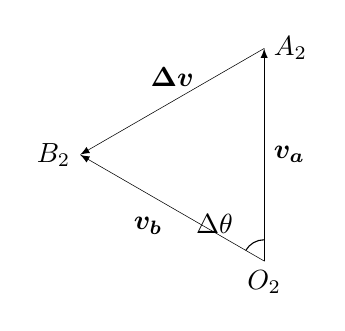
\begin{tikzpicture}[scale=0.9]
                        \tkzDefPoint(0,0){O}
                        \tkzDefPoint(90:3){A}
                        \tkzDefPoint(150:3){B}

                        \tkzDrawSegment[-latex](O,A)
                        \tkzDrawSegment[-latex](O,B)
                        \tkzDrawSegment[-latex](A,B)

                        \tkzLabelPoint[below](O){$O_2$}
                        \tkzLabelPoint[right](A){$A_2$}
                        \tkzLabelPoint[left](B){$B_2$}

                        \tkzLabelSegment[right](O,A){$\veb{v_a}$}
                        \tkzLabelSegment[below left](O,B){$\veb{v_b}$}
                        \tkzLabelSegment[above=2pt](A,B){$\veb{\Delta v}$}

                        \tkzLabelPoint(-0.7,0.8){$\Delta\theta$}
                        \tkzMarkAngle[size=0.3](A,O,B)
                    \end{tikzpicture}
                \end{minipage}
            }
            \caption{匀速圆周运动的示意图}
        \end{center}
    \end{figure}\\
    显然线速度可以表示为:
    \setcounter{equation}{0}
    \begin{align}
        v=|\veb{v_a}|
    \end{align}\\
    由于$\triangle O_2A_2B_2\simeq\triangle O_1A_1B_1$:\vspace{5pt}
    \begin{align}
        &\frac{A_2B_2}{A_2O_2}=\frac{A_1B_1}{A_1O_1}\\[3mm]
        &\frac{\Delta v}{v}=\frac{\Delta r}{r}\\[3mm]
        &\frac{\Delta v}{\Delta t}=\frac{v}{r}\cdot\frac{\Delta r}{\Delta t}
    \end{align}\\
    此步利用了速度三角形和位移三角形相似的原理。

\newpage

    根据定义可以求得向心加速度$a$:
    \begin{align}
        a
        &=\lim_{\Delta t\rightarrow 0}\frac{\Delta v}{\Delta t}\\[3mm]
        &=\lim_{\Delta t\rightarrow 0}\frac{v}{r}\cdot\frac{\Delta r}{\Delta t}\\[3mm]
        &=\lim_{\Delta t\rightarrow 0}\frac{v}{r}\cdot\frac{\Delta s}{\Delta t}\\[3mm]
        &=\frac{v}{r}\cdot\frac{\dif s}{\dif t}\\[3mm]
        &=\frac{v^2}{r}
    \end{align}\\
    向心加速度的计算公式:
    \begin{large}
        \begin{equation*}
            a=\frac{v^2}{r}    
        \end{equation*}
    \end{large}\\
    向心加速度的方向始终指向圆心。\\[3mm]
    向心加速度的方向为$\veb{\Delta v}\rightarrow 0$时的方向,当$\Delta t\rightarrow 0$,有$\Delta\theta\rightarrow 0$,此时$\veb{\Delta v}$趋向于与$\veb{v_a}$垂直。

\newpage

\subsubsection{线量描述下的变速圆周运动}
    变速圆周运动可以通过两个线量描述,线速度$v$,法向加速度$a_n$,切向加速度$a_t$。\\[3mm]
    变速圆周运动的示意图中,速度$\veb{v_a}$是矢量$O_2A_2$,速度$\veb{v_b}$是矢量$O_2B_3$。\\[3mm]
    变速圆周运动的示意图:\vspace{5pt}
    \setcounter{subfigure}{0}
    \begin{figure}[h]
        \begin{center}
            \subfigure[位移示意图]
            {
                \begin{minipage}[t]{0.36\linewidth}
                    \begin{tikzpicture}[scale=0.9]
                        \tkzDefPoint(0,0){O}
                        \tkzDefPoint(0:3){A}
                        \tkzDefPoint(60:3){B}

                        \tkzDrawCircle(O,A)
                        \tkzDrawSegment(O,A)
                        \tkzDrawSegment(O,B)
                        \tkzDrawSegment[dashed,-latex](A,B)

                        \tkzMarkAngle[size=0.3](A,O,B)

                        \tkzLabelSegment[below](O,A){$r$}
                        \tkzLabelSegment[below left](A,B){$\veb{\Delta r}$}
                        \tkzLabelSegment[pos=0.8,above right=4pt](A,B){$~\Delta s$}

                        \tkzDefLine[orthogonal=through A](O,A)
                        \tkzGetPoint{a}

                        \tkzDefLine[orthogonal=through B](O,B)
                        \tkzGetPoint{b}
                        
                        \tkzDrawSegment[-latex,add=0 and -0.25](A,a)
                        \tkzDrawSegment[-latex](B,b)

                        \tkzDefShiftPoint[a](0,-0.7){a2}

                        \tkzLabelPoint[right](a2){$\veb{v_a}$}
                        \tkzLabelPoint[above right](b){$\veb{v_b}$}

                        \tkzLabelPoint(0.2,0.6){$\Delta\theta$}
                        \tkzLabelPoint[below](O){$O_1$}
                        \tkzLabelPoint[below right](A){$A_1$}
                        \tkzLabelPoint[above](B){$B_1$}
                    \end{tikzpicture}
                \end{minipage}
            }\qquad\qquad\qquad
            \subfigure[速度示意图]
            {
                \begin{minipage}[t]{0.342\linewidth}
                    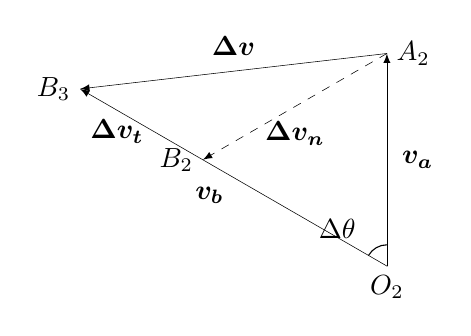
\begin{tikzpicture}[scale=0.9]
                        \tkzDefPoint(0,0){O}
                        \tkzDefPoint(90:3){A}
                        \tkzDefPoint(150:3.0){B2}
                        \tkzDefPoint(150:5){B3}

                        \tkzDrawSegment[-latex](O,A)
                        \tkzDrawSegment[-latex](O,B3)
                        \tkzDrawSegment[-latex](A,B3)
                        \tkzDrawSegment[-latex,dashed](A,B2)

                        \tkzLabelPoint[below](O){$O_2$}
                        \tkzLabelPoint[right](A){$A_2$}
                        \tkzLabelPoint[left](B2){$B_2$}
                        \tkzLabelPoint[left](B3){$B_3$}

                        \tkzLabelSegment[right=2pt](O,A){$\veb{v_a}$}
                        \tkzLabelSegment[below left](O,B3){$\veb{v_b}$}
                        \tkzLabelSegment[above=2pt](A,B3){$\veb{\Delta v}$}
                        \tkzLabelSegment[below=2pt](A,B2){$\veb{\Delta v_n}$}
                        \tkzLabelSegment[below,pos=0.7](B2,B3){$\veb{\Delta v_t}$}

                        \tkzLabelPoint(-0.7,0.8){$\Delta\theta$}
                        \tkzMarkAngle[size=0.3](A,O,B2)
                    \end{tikzpicture}
                \end{minipage}
            }
            \caption{变速圆周运动的示意图}
        \end{center}
    \end{figure}\\
    显然线速度可以表示为:
    \setcounter{equation}{0}
    \begin{align}
        v=|\veb{v_a}|
    \end{align}\\
    由于$\triangle O_2A_2B_2\simeq\triangle O_1A_1B_1$:\vspace{5pt}
    \begin{align}
        &\frac{A_2B_2}{A_2O_2}=\frac{A_1B_1}{A_1O_1}\\[3mm]
        &\frac{\Delta v_n}{v}=\frac{\Delta r}{r}\\[3mm]
        &\frac{\Delta v_n}{\Delta t}=\frac{v_n}{r}\cdot\frac{\Delta r}{\Delta t}
    \end{align}\\
    此步利用了速度三角形和位移三角形相似的原理。

\newpage

    根据定义可以求得法向加速度$a_n$:
    \begin{align}
        a_n
        &=\lim_{\Delta t\rightarrow 0}\frac{\Delta v_n}{\Delta t}\\[3mm]
        &=\lim_{\Delta t\rightarrow 0}\frac{v_n}{r}\cdot\frac{\Delta r}{\Delta t}\\[3mm]
        &=\lim_{\Delta t\rightarrow 0}\frac{v_n}{r}\cdot\frac{\Delta s}{\Delta t}\\[3mm]
        &=\frac{v}{r}\cdot\frac{\dif s}{\dif t}\\[3mm]
        &=\frac{v^2}{r}
    \end{align}\\
    法向加速度的计算公式:
    \begin{large}
        \begin{equation*}
            a_n=\frac{v^2}{r}
        \end{equation*}
    \end{large}\\
    法向加速度的方向始终指向圆心。\\[3mm]
    法向加速度的方向为$\veb{\Delta v_n}\rightarrow 0$时的方向,当$\Delta t\rightarrow 0$,有$\Delta\theta\rightarrow 0$,此时$\veb{\Delta v}$趋向于与$\veb{v_a}$垂直。\\[12mm]
    根据定义可以求得切向加速度$a_t$:
    \begin{align}
        a_t
        &=\lim_{\Delta t\rightarrow 0}\frac{\Delta v_t}{\Delta t}\\[3mm]
        &=\lim_{\Delta t\rightarrow 0}\frac{v_b-v_a}{r}\\[3mm]
        &=\lim_{\Delta t\rightarrow 0}\frac{\Delta v}{r}\\[3mm]
        &=\frac{\dif v}{\dif t}
    \end{align}\\
    切向加速度的计算公式:
    \begin{large}
        \begin{equation*}
            a_t=\frac{\dif v}{\dif t}
        \end{equation*}
    \end{large}\\
    切向加速度的方向始终指向圆心。\\[3mm]
    切向加速度的方向为$\veb{\Delta v_t}\rightarrow 0$时的方向,当$\Delta t\rightarrow 0$,有$\Delta\theta\rightarrow 0$,此时$\veb{\Delta v_t}$趋向于与$\veb{v_a}$平行。

\newpage

\subsubsection{线量和角量的关系}
    \setcounter{equation}{0}
    线速度和角量的关系:
    \begin{large}
        \begin{equation*}
            v=r\cdot\omega
        \end{equation*}
    \end{large}\\
    法向加速度和角量的关系:
    \begin{large}
        \begin{equation*}
            a_n=r\cdot\omega^2
        \end{equation*}
    \end{large}\\
    切向加速度和角量的关系:
    \begin{large}
        \begin{equation*}
            a_t=r\cdot\alpha
        \end{equation*}
    \end{large}\\
    即法向加速度是半径和角速度平方的乘积,而切向加速度是半径和角加速度的乘积。\\[12mm]
    由于线速度可以表示为:
    \begin{align}
        v=\lim_{\Delta t\rightarrow 0}\frac{\Delta s}{\Delta t}=\frac{\dif s}{\dif t}
    \end{align}\\
    由于角速度可以表示为:
    \begin{align}
        \omega=\lim_{\Delta t\rightarrow 0}\frac{\Delta\theta}{\Delta t}=\frac{\dif \theta}{\dif t}
    \end{align}\\
    同时因为存在以下关系:
    \begin{align}
        \dif s=r\cdot\dif \theta
    \end{align}\\
    因此可以得到:
    \begin{align}
        &\frac{v}{\omega}=\frac{\dif s}{\dif \theta}\\[5mm]
        &\frac{v}{\omega}=\frac{r\cdot \dif \theta}{\dif \theta}\\[5mm]
        &\frac{v}{\omega}=r\\[5mm]
        &v=r\cdot\omega
    \end{align}\\
    由此证明了线速度和角速度的关系。

\newpage

    代入法向加速度的公式:
    \begin{align}
        a_n
        &=\frac{v^2}{r}\\[3mm]
        &=\frac{~r^2\cdot\omega^2}{r}\\[3mm]
        &=r\cdot\omega^2
    \end{align}\\
    代入切向加速度的公式:
    \begin{align}
        a_t
        &=\frac{\dif v}{\dif t}\\[3mm]
        &=r\cdot\frac{\dif \omega}{\dif t}\\[3mm]
        &=r\cdot\alpha
    \end{align}\\
    由此证明了法向加速度和角速度的关系。\\[3mm]
    由此证明了切向加速度和角加速度的关系。

\newpage

\subsection{抛体运动}
    抛体运动指的是物体以一定初速度抛出后,仅在重力作用下所做的运动。\\[3mm]
    抛体运动的示意图:\vspace{5pt}
    \begin{figure}[h]
        \begin{center}
            \begin{tikzpicture}[scale=1.5]
                \tkzDefPoint(0,0){O}
                \tkzDefPoint(6,0){X}
                \tkzDefPoint(0,4.5){Y}

                \tkzDrawSegment[->](O,X)
                \tkzDrawSegment[->](O,Y)

                \tkzLabelPoint[left](O){$O$}
                \tkzLabelPoint[right](X){$X$}
                \tkzLabelPoint[left](Y){$Y$}

                \tkzDefPoint(5.5,3.0){g1}
                \tkzDefPoint(5.5,2.5){g2}

                \tkzDrawSegment[-latex](g1,g2)
                \tkzLabelPoint[right](g2){$g$}

                \draw[smooth,thick,samples=100,domain=0:5] plot(\x,{-0.4*\x*\x+2*\x});

                \tkzDefPoint(1.5,3.0){V}
                \tkzDrawSegment[-latex](O,V)

                \tkzLabelPoint[above right](V){$v_0$}

                \tkzMarkAngle[size=0.3](X,O,V)
                \tkzLabelPoint(0.5,0.5){$\theta_0$}
            \end{tikzpicture}
            \caption{抛体运动的示意图}
        \end{center}
    \end{figure}\\
    以水平方向为$X$轴,竖直方向为$Y$轴,建立平面直角坐标系。\\[3mm]
    设一质点由原点$O$抛出,其初速度为$v_0$,其与水平方向的初角度为$\theta_0$。\\[6mm]
    抛体运动可以视为两个方向上运动的叠加:\\[3mm]
    在水平方向上,抛出物体不受力的作用,因此在水平方向上作匀速直线运动。\\[3mm]
    在竖直方向上,抛出物体仅受重力作用,因此在竖直方向上作匀变速直线运动。\\[3mm]

\newpage

\subsubsection{抛体运动的运动学方程}
    \setcounter{equation}{0}
    其初速$v$在$X$轴上的分量$v_{0x}$:
    \begin{align}
        v_{0x}=v_0\cdot\cos{\theta_0}
    \end{align}\\
    其初速$v$在$Y$轴上的分量$v_{0y}$:
    \begin{align}
        v_{0y}=v_0\cdot\sin{\theta_0}
    \end{align}\\
    故速度可以表示为:
    \begin{align}
        \begin{cases}
            ~v_x=v_0\cdot\cos{\theta_0}\\[1mm]
            ~v_y=v_0\cdot\sin{\theta_0}-g\cdot t\\[1mm]
        \end{cases}
    \end{align}\\
    故位矢可以表示为:
    \begin{align}
        ~~~~~~~~~~
        \begin{cases}
            ~x=v_0\cdot\cos{\theta_0}\cdot t\\[1mm]
            ~y=v_0\cdot\,\sin{\theta_0}\cdot t-\dfrac{1}{2}\cdot g\cdot t^2\\[1mm]
        \end{cases}
    \end{align}\\
    消去参数即可得到:
    \begin{align}
        &t=\frac{x}{v_0\cdot\cos{\theta_0}}\\[5mm]
        &y=v_0\cdot\sin{\theta_0}\cdot t-\frac{1}{2}\cdot g\cdot t^2\\[5mm]
        &y=\frac{v_0\cdot\sin{\theta_0}}{v_0\cdot\cos{\theta_0}}\cdot x-\frac{g}{2\cdot v_0^2\cdot\cos^2{\theta_0}}\cdot x^2\\[5mm]
        &y=x\cdot\tan{\theta_0}-x^2\cdot\frac{g}{2\cdot v_0^2\cdot\cos{\theta_0}}
    \end{align}\\
    故抛体运动的轨迹方程:
    \begin{large}
        \begin{equation*}
            y=x\cdot\tan{\theta_0}-x^2\cdot\frac{g}{2\cdot v_0^2\cdot\cos{\theta_0}}
        \end{equation*}
    \end{large}\\
    该方程中,$x$有一次项和二次项,$y$只有一次项,故抛体运动的轨迹为抛物线。

\newpage

\subsubsection{抛体运动的滞空时间}
    \setcounter{equation}{0}
    抛体运动的滞空时间:
    \begin{large}
        \begin{equation*}
            T=\frac{2\cdot v_0\cdot\sin{\theta_0}}{g}~~~~~
        \end{equation*}
    \end{large}\\
    抛体运动的最大滞空时间:
    \begin{large}
        \begin{equation*}
            ~~~~~~~~T_{max}=\frac{2\cdot v_0}{g}~~~~\left(\theta=\frac{\pi}{2}\right)
        \end{equation*}
    \end{large}\\
    根据$y$轴上的运动学方程:
    \begin{align}
        &y=v_0\cdot\sin{\theta_0}\cdot t-\frac{1}{2}\cdot g\cdot t^2\\[4mm]
        &0=v_0\cdot\sin{\theta_0}\cdot t-\frac{1}{2}\cdot g\cdot t^2\\[4mm]
        &0=-\frac{1}{2}\cdot g\cdot t^2+v_0\cdot\sin{\theta_0}\cdot t
    \end{align}\\
    解方程可得:
    \begin{align}
        &t=\frac{-v_0\cdot\sin{\theta_0}\pm\sqrt{v_0^2\cdot\sin^2{\theta_0}}}{-g}\\[4mm]
        &t_1=\frac{-v_0\cdot\sin{\theta_0}+v_0\cdot\sin{\theta_0}}{-g}=0\\[4mm]
        &t_2=\frac{-v_0\cdot\sin{\theta_0}-v_0\cdot\sin{\theta_0}}{-g}=T
    \end{align}\\
    化简整理可得:
    \begin{align}
        &T=\frac{-v_0\cdot\sin{\theta_0}-v_0\cdot\sin{\theta_0}}{-g}\\[3mm]
        &T=\frac{-2\cdot v_0\cdot\sin{\theta_0}}{-g}\\[3mm]
        &T=\frac{2\cdot v_0\cdot\sin{\theta_0}}{g}
    \end{align}\\
    故当$v_0$一定时,当$\theta=\dfrac{\pi}{2}$时有最大滞空时间。

\newpage

\newpage

\subsubsection{抛体运动的高度}
    \setcounter{equation}{0}
    抛体运动的高度:
    \begin{large}
        \begin{equation*}
            H=\frac{v_0^2\cdot\sin^2{\theta_0}}{2g}~~~~~
        \end{equation*}
    \end{large}\\
    抛体运动的最大高度:
    \begin{large}
        \begin{equation*}
            ~~~~~~~~H_{max}=\frac{v_0^2}{2g}~~~~\left(\theta_0=\frac{\pi}{2}\right)
        \end{equation*}
    \end{large}\\
    代入滞空时间可得:
    \begin{align}
        &H=v_0\cdot\cos{\theta_0}\cdot\frac{T}{2}-\frac{1}{2}\cdot g\cdot \frac{T^2}{4}\\[4mm]
        &H=\frac{1}{2}\cdot v_0\cdot\cos{\theta_0}\cdot T-\frac{1}{8}\cdot g\cdot T^2\\[4mm]
        &H=\frac{v_0^2\cdot\sin^2{\theta_0}}{g}-\frac{v_0^2\cdot\sin^2{\theta_0}}{2g}\\[4mm]
        &H=\frac{2\cdot v_0^2\cdot\sin^2{\theta_0}}{2g}-\frac{v_0^2\cdot\sin^2{\theta_0}}{2g}\\[4mm]
        &H=\frac{v_0^2\cdot\sin^2{\theta_0}}{2g}
    \end{align}\\
    故当$v_0$一定时,当$\theta=\dfrac{\pi}{2}$时有最大射程。

\newpage

\subsubsection{抛体运动的射程}
    \setcounter{equation}{0}
    抛体运动的射程:
    \begin{large}
        \begin{equation*}
            R=\frac{v_0^2\cdot\sin{2\theta_0}}{g}~~~~~
        \end{equation*}
    \end{large}\\
    抛体运动的最大射程:
    \begin{large}
        \begin{equation*}
            ~~~~~~~~R_{max}=\frac{v_0^2}{g}~~~~\left(\theta_0=\frac{\pi}{4}\right)
        \end{equation*}
    \end{large}\\
    代入滞空时间可得:
    \begin{align}
        &R=v_0\cdot\cos{\theta_0}\cdot T\\[4mm]
        &R=\frac{2\cdot v_0^2\cdot\cos{\theta_0}\cdot\sin{\theta_0}}{g}\\[4mm]
        &R=\frac{v_0^2\cdot\sin{2\theta_0}}{g}
    \end{align}\\
    故当$v_0$一定时,当$\theta=\dfrac{\pi}{4}$时有最大射程。

\newpage

\section{运动定律}
    根据观察和实验,有两个因素影响着物体的机械运动:\\[3mm]
    1.物体本身的固有属性,称其为质量。\\[3mm]
    2.物体之间的相互作用,称其为力。

\subsection{质量}
    质量衡量了物体的引力特性和惯性特性的强弱,是一个标量,通常用符号$m$表示,单位是\si{kg}。\\[3mm]
    质量反应了两个不同性质:\\[3mm]
    1.质量反应了物体引力特性的强弱,质量越大引力越大,这种质量称为引力质量。\\[3mm]
    2.质量反应了物体惯性特性的强弱,质量越大惯性越大,这种质量称为惯性质量。\\[3mm]
    其中惯性指的是改变物体运动状态的难易程度。\\[3mm]
    虽然引力质量和惯性质量的含义不同,但是物理研究表明两种质量可不予区分。

\subsection{力}
    力衡量了物体间相互作用的强弱,是一个矢量,通常用符号$\veb{F}$表示,单位是\si{N}。\\[3mm]
    力的单位牛顿的定义如下:
    \begin{large}
        \begin{center}
            \si{N=kg\cdot m/s^2}\\[6mm]
        \end{center}
    \end{large}
    力的作用效果有两种:使受力物体的运动状态发生改变,使受体物体发生形变。\\

\subsubsection{牛顿第一定律}
    \textbf{牛顿第一定律:}任何物体都将保持静止或匀速直线运动,直到外力迫使它改变这种状态为止。\\[3mm]
    牛顿第一定律揭示了两个重要事实:\\[3mm]
    1.物体具有保持其运动状态不变的性质。\\[3mm]
    2.物体运动状态改变的原因是力。\\[3mm]
    力是改变物体运动状态的原因,力不是维持物体运动状态的原因。

\newpage

\subsubsection{牛顿第二定律}
    \textbf{牛顿第二定律:}当力作用于物体时,物体所得到的加速度的大小,与物体所受的合力成正比,\\
    与物体的质量成反比,物体加速度的方向与物体所受的合外力方向相同。\\[3mm]
    牛顿第二定律的数学表达:
    \begin{large}
        \begin{equation*}
            \veb{F}=m\cdot\veb{a}
        \end{equation*}
    \end{large}\\
    牛顿二定律的直角坐标分量式:\vspace{5pt}
    \begin{large}
        \begin{equation*}
            \begin{cases}
                ~F_x=m\cdot a_x\\[1mm]
                ~F_y=m\cdot a_y\\[1mm]
                ~F_z=m\cdot a_z\\[1mm]
            \end{cases}
        \end{equation*}
    \end{large}\\
    牛顿二定律的法向切向分量式:\vspace{5pt}
    \begin{large}
        \begin{equation*}
            \begin{cases}
                ~F_n=m\cdot a_n\\[1mm]
                ~F_t\,=m\cdot a_t\\[1mm]
            \end{cases}
        \end{equation*}
    \end{large}\\
    牛顿第二定律定量的说明了:\\[3mm]
    1.质量和力对物体加速度的影响。\\[3mm]
    2.质量是物体惯性的量度。\\

\subsubsection{牛顿第三定律}
    \textbf{牛顿第三定律:}相互作用的两个物体之间的作用力和反作用力,大小相等,方向相反。\\[3mm]
    牛顿第三定律的数学表达:
    \begin{large}
        \begin{equation*}
            \veb{F_{AB}}+\veb{F_{BA}}=0
        \end{equation*}
    \end{large}\\
    牛顿第三定律说明了物体间力的性质:\\[3mm]
    1.作用力和反作用力总是同时出现同时消失。\\[3mm]
    2.作用力和反作用力总是同一类型的力。

\newpage

\subsubsection{惯性系和非惯性系}
    凡是可以适用牛顿运动定律的参照系,称为惯性系。\\[3mm]
    凡是不能适用牛顿运动定律的参照系,称为非惯性系。\\[6mm]
    相较于一个惯性系的加速度为$\veb{a}=0$的参照系,也是一个惯性系。\\[3mm]
    相较于一个惯性系的加速度为$\veb{a}\neq 0$的参照系,则是一个非惯性系。\\[6mm]
    非惯性系中运动定律不再适用,但是我们可以通过添加惯性力,使运动定律重新适用。\\[3mm]
    非惯性系中的惯性力:
    \begin{large}
        \begin{equation*}
            \veb{F_{\text{惯}}}=-m\cdot \veb{a}
        \end{equation*}
    \end{large}\\
    其中$\veb{a}$为该非惯性系相对于惯性系的加速度。\\[3mm]
    惯性力的方向始终和非惯性系加速度的方向相反。\\[3mm]
    惯性力是一个虚拟的力,无施力物体,无反作用力。\\[6mm]
    运用惯性力可以解释失重和超重的现象:\vspace{5pt}
    \begin{figure}[h]
        \begin{center}
            \subfigure[失重]
            {
                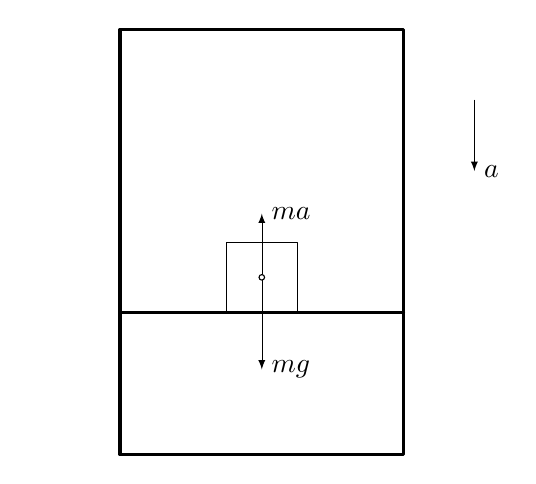
\begin{tikzpicture}[scale=0.9]
                    \tkzDefPoint(-2,+6){E1}
                    \tkzDefPoint(+2,+6){E2}
                    \tkzDefPoint(-2,0){E3}
                    \tkzDefPoint(+2,0){E4}
                    \tkzDrawPolygon[very thick](E1,E2,E4,E3)

                    \tkzDefPoint(-2,2.0){F1}
                    \tkzDefPoint(+2,2.0){F2}
                    \tkzDrawSegment[very thick](F1,F2)

                    \tkzDefPoint(0,2.5){G}
    
                    \tkzDefShiftPoint[G](-0.5,+0.5){B1}
                    \tkzDefShiftPoint[G](+0.5,+0.5){B2}
                    \tkzDefShiftPoint[G](-0.5,-0.5){B3}
                    \tkzDefShiftPoint[G](+0.5,-0.5){B4}
                    \tkzDrawPolygon(B1,B2,B4,B3)

                    \tkzDefShiftPoint[G](0,-1.3){FG}
                    \tkzDefShiftPoint[G](0,+0.9){FA}

                    \tkzDrawSegment[-latex](G,FG)
                    \tkzDrawSegment[-latex](G,FA)

                    \tkzDrawPoint[fill=white](G)

                    \tkzLabelPoint[right](FG){$mg$}
                    \tkzLabelPoint[right](FA){$ma$}

                    \tkzDefPoint(+3.0,4){A1}
                    \tkzDefPoint(+3.0,5){A2}
                    \tkzDrawSegment[-latex](A2,A1)
                    \tkzLabelPoint[right](A1){$a$}

                    \tkzDefPoint(-3.3,4){A3}
                    \tkzDefPoint(-3.3,5){A4}
                    \tkzDrawSegment[white](A3,A4)
                \end{tikzpicture}
            }
            \subfigure[超重]
            {
                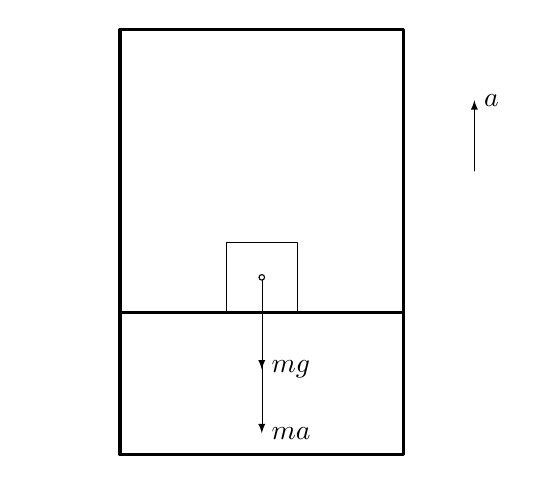
\begin{tikzpicture}[scale=0.9]
                    \tkzDefPoint(-2,+6){E1}
                    \tkzDefPoint(+2,+6){E2}
                    \tkzDefPoint(-2,0){E3}
                    \tkzDefPoint(+2,0){E4}
                    \tkzDrawPolygon[very thick](E1,E2,E4,E3)

                    \tkzDefPoint(-2,2.0){F1}
                    \tkzDefPoint(+2,2.0){F2}
                    \tkzDrawSegment[very thick](F1,F2)

                    \tkzDefPoint(0,2.5){G}
    
                    \tkzDefShiftPoint[G](-0.5,+0.5){B1}
                    \tkzDefShiftPoint[G](+0.5,+0.5){B2}
                    \tkzDefShiftPoint[G](-0.5,-0.5){B3}
                    \tkzDefShiftPoint[G](+0.5,-0.5){B4}
                    \tkzDrawPolygon(B1,B2,B4,B3)

                    \tkzDefShiftPoint[G](0,-1.3){FG}
                    \tkzDefShiftPoint[G](0,-2.2){FA}

                    \tkzDrawSegment[-latex](G,FG)
                    \tkzDrawSegment[-latex](G,FA)

                    \tkzDrawPoint[fill=white](G)

                    \tkzLabelPoint[right](FG){$mg$}
                    \tkzLabelPoint[right](FA){$ma$}

                    \tkzDefPoint(+3.0,4){A1}
                    \tkzDefPoint(+3.0,5){A2}
                    \tkzDrawSegment[-latex](A1,A2)
                    \tkzLabelPoint[right](A2){$a$}

                    \tkzDefPoint(-3.3,4){A3}
                    \tkzDefPoint(-3.3,5){A4}
                    \tkzDrawSegment[white](A3,A4)
                \end{tikzpicture}
            }
            \caption{超重和失重}
        \end{center}
    \end{figure}\\
    当电梯加速度向下时,其中的物体受到一个向上的惯性力,抵消了部分重力,因此观察到失重。\\[3mm]
    当电梯加速度向上时,其中的物体受到一个向下的惯性力,加强了部分重力,因此观察到超重。

\newpage

\subsection{力学中常见的力}
    力学中常见的力包含三种:重力,弹力,摩擦力。

\subsubsection{重力}
    重力指的是物体由于受到地球吸引而受到的,通常用字母$G$表示。\\[3mm]
    重力的方向总是竖直向下垂直于当地的水平面。\\[3mm]
    重力的计算公式:
    \begin{large}
        \begin{equation*}
            G=-m\cdot g
        \end{equation*}
    \end{large}\\
    其中$g$为当地的重力加速度,物体所受重力的大小和质量成正比。\\[3mm]
    如果以竖直向上为正方向,则重力方向始终为负,这就是公式中负号的含义。\\

\subsubsection{弹力}
    弹力指的是物体由于发生弹性形变而产生的力,通常用字母$F$表示。\\[3mm]
    弹力的方向总是与物体发生形变的方向相反。\\[3mm]
    弹力的计算公式(胡克定律):
    \begin{large}
        \begin{equation*}
            F=-k\cdot x
        \end{equation*}
    \end{large}\\
    其中$k$为弹簧的劲度系数,物体所受弹力的大小和形变程度成正比。\\[3mm]
    如果以位移方向为正方向,则弹力方向始终为负,这就是公式中负号的含义。\\[6mm]
    除了弹簧产生的弹力,一般的物体发生形变也可以产生弹力:\\[3mm]
    1.压力指的是物体间由于相互挤压发生形变而产生的力,通常用字母$N$表示。\\[3mm]
    2.张力指的是线绳内由于发生了伸长的形变而产生的力,通常用字母$T$表示。\\[3mm]

\newpage

\subsubsection{摩擦力}
    摩擦力指的是两个粗糙物体由于相互摩擦而产生的力,通常用字母$f$表示。\\[3mm]
    摩擦力具体可以分为两种:滑动摩擦力和静摩擦力。\\[3mm]
    \textbf{1.动摩擦力}\\[2mm]
    滑动摩擦力指的是两个粗糙物体由于相对滑动而产生的力,通常用$f_k$表示。\\[3mm]
    滑动摩擦力的方向总是沿着接触面的切线方向,且与物体相对运动方向相反。\\[3mm]
    滑动摩擦力的计算公式:
    \begin{large}
        \begin{equation*}
            f_{k}=\mu_k\cdot N
        \end{equation*}
    \end{large}\\
    其中$\mu_k$为动摩擦系数,物体所受动摩擦力的大小和物体间的弹力成正比。\\[8mm]
    \textbf{2.静摩擦力}\\[2mm]
    静摩擦力指的是两个粗糙物体由于相对滑动趋势而产生的力,通常用$f_s$表示。\\[3mm]
    静摩擦力的方向总是沿着接触面的切线方向,且与物体的相对运动趋势方向相反。\\[3mm]
    静摩擦力的大小与物体间弹力无关,而是与外力的大小保持相同,使得物体能够始终保持静止,
    随着外力逐渐增大,静摩擦力逐渐增大,直至物体发生运动。\\[3mm]
    最大静摩擦力指的是物体在发生运动前可以产生的最大的静摩擦力。\\[3mm]
    最大静摩擦力的计算公式:
    \begin{large}
        \begin{equation*}
            f_{s}=\mu_{s}\cdot N
        \end{equation*}
    \end{large}\\
    其中$\mu_s$为静摩擦系数,物体所受最大静摩擦力的大小和物体间的弹力成正比。\\[6mm]
    通常来说,静摩擦因数和动摩擦因数小于一,即$\mu_s<1$且$\mu_k<1$。\\[3mm]
    实验表明,静摩擦因数总是大于动摩擦因数,即$\mu_s>\mu_k$。\\[3mm]
    这一特点意味着,使物体开始运动所需的力大于维持物体匀速直线运动所需的力。

\newpage

\section{能量守恒定律}

\subsection{功}
    功衡量了力在空间上的积累,是一个标量,通常用符号$W$表示,单位是\si{J}。\\[3mm]
    功的单位焦耳定义如下:
    \begin{large}
        \begin{align*}
            &\si{J=N\cdot m}\\[3mm]
            &\si{J=kg\cdot m^2/s^2}
        \end{align*}
    \end{large}\\
    功的计算公式(恒力做功):
    \begin{large}
        \begin{align*}
            &W=\veb{F}\cdot\veb{s}\\[3mm]
            &W=F\cdot s\cdot\cos{\theta}
        \end{align*}
    \end{large}\\
    功的计算公式(变力做功):
    \begin{large}
        \begin{align*}
            &W=\int_{\veb{s_1}}^{\veb{s_2}}\veb{F}\cdot\dif\veb{s}\\[3mm]
            &W=\int_{s_1}^{s_2}F\cdot\dif s\cdot\cos{\theta}
        \end{align*}
    \end{large}\\
    其中角$\theta$代表力$\veb{F}$和位移$\veb{s}$间的夹角。\\[5mm]
    同时角$\theta$的大小决定了功$W$的正负:\vspace{5pt}
    \begin{table}[h]
        \begin{center}
            \begin{tabular}{p{80pt}|p{160pt}}
                \hline
                满足$\theta<\dfrac{\pi}{2}$\vphantom{$\Biggl(\Biggr)$}&功为正,表示力对物体做正功。\\ \hline
                满足$\theta>\dfrac{\pi}{2}$\vphantom{$\Biggl(\Biggr)$}&功为负,表示力对物体做负功。\\ \hline
            \end{tabular}
            \caption{角$\theta$的大小和功的正负}
        \end{center}
    \end{table}\\
    此外,若力的方向和位移的方向垂直,则力不做功。

\newpage

\subsection{功率}
    功率衡量了力做功的快慢,是一个标量,通常用字母$P$表示,单位是\si{W}。\\[3mm]
    功率的单位瓦特的定义如下:
    \begin{large}
        \begin{align*}
            &\si{W=J/s}\\[3mm]
            &\si{W=N\cdot m/s}\\[3mm]
            &\si{W=kg\cdot m^2/s^3}
        \end{align*}
    \end{large}\\
    功率是功关于时间的导数:
    \setcounter{equation}{0}
    \begin{align}
        P
        &=\frac{\dif W}{\dif t}\\[3mm]
        &=\frac{\dif}{\dif t}\cdot\int\veb{F}\cdot\dif\veb{s}\\[3mm]
        &=\frac{\dif}{\dif t}\cdot\int\veb{F}\cdot\veb{v}\cdot\dif t\\[3mm]
        &=\veb{F}\cdot\veb{v}
    \end{align}\\
    功率的计算公式:
    \begin{large}
        \begin{align*}
            &P=\veb{F}\cdot\dif\veb{v}\\[3mm]
            &P=F\cdot\dif v\cdot\cos{\theta}
        \end{align*}
    \end{large}\\
    其中角$\theta$代表力$\veb{F}$和速度$\veb{v}$间的夹角。\\[5mm]
    同时角$\theta$的大小决定了功率$P$的正负:\vspace{8pt}
    \begin{table}[h]
        \begin{center}
            \begin{tabular}{p{80pt}|p{220pt}}
                \hline
                满足$\theta<\dfrac{\pi}{2}$\vphantom{$\Biggl(\Biggr)$}&功率为正,表示在这一瞬间力对物体做正功。\\ \hline
                满足$\theta>\dfrac{\pi}{2}$\vphantom{$\Biggl(\Biggr)$}&功率为负,表示在这一瞬间力对物体做负功。\\ \hline
            \end{tabular}
            \caption{角$\theta$的大小和功率的正负}
        \end{center}
    \end{table}\\
    此外,若力的方向和速度的方向垂直,则力的功率为零。

\newpage

\subsection{能}
    能衡量了物体做功本领的强弱,是一个标量,通常用符号$E$表示,单位是\si{J}。\\[3mm]
    能的单位焦耳定义如下:
    \begin{large}
        \begin{align*}
            &\si{J=N\cdot m}\\[3mm]
            &\si{J=kg\cdot m^2/s^2}
        \end{align*}
    \end{large}\vspace{-10pt}

\subsubsection{动能}
    动能指的是物体由于运动而具有的能力,通常用符号$E_k$表示。\\[3mm]
    动能定义为物体从速度为$0$时至速度为$v$时外力所作的功。\\[3mm]
    动能的计算公式:
    \begin{large}
        \begin{equation*}
            E_k=\frac{1}{2}\cdot m\cdot v^2
        \end{equation*}
    \end{large}\\
    由功的计算公式进行推导:
    \setcounter{equation}{0}
    \begin{align}
        W
        &=\int_{\veb{s_1}}^{\veb{s_2}}\veb{F}\cdot\dif\veb{s}\\[3mm]
        &=\int_{t_1}^{t_2}\veb{F}\cdot\veb{v}\cdot\dif t\\[3mm]
        &=\int_{t_1}^{t_2}m\cdot\veb{a}\cdot\veb{v}\cdot\dif t\\[3mm]
        &=\int_{\veb{v_1}}^{\veb{v_2}}m\cdot\frac{\dif\veb{v}}{\dif t}\cdot\veb{v}\cdot\dif t\\[3mm]
        &=\int_{\veb{v_1}}^{\veb{v_2}}m\cdot\veb{v}\cdot\dif\veb{v}\\[3mm]
        &=\frac{1}{2}\cdot m\cdot \veb{v_2}^2-\frac{1}{2}\cdot m\cdot \veb{v_1}^2\\[3mm]
        &=\frac{1}{2}\cdot m\cdot v_2^2-\frac{1}{2}\cdot m\cdot v_1^2
    \end{align}\\
    根据动能定义,初速度应为$v_1=0$,末速度应为$v_2=v$,代入即可得到动能的公式。\\[3mm]

\newpage

\subsubsection{重力势能}
    重力势能指的是物体由于重力而具有的能量,通常用字母$E_p$表示。\\[3mm]
    重力势能定义为物体从高度为$h$处至高度为$0$处重力所做的功。\\[3mm]
    重力势能的计算公式:
    \begin{large}
        \begin{equation*}
            E_p=m\cdot g\cdot h
        \end{equation*}
    \end{large}\\
    由功的计算公式进行推导:
    \setcounter{equation}{0}
    \begin{align}
        W
        &=\int_{h_1}^{h_2}G\cdot\dif h\\[3mm]
        &=\int_{h_1}^{h_2}-m\cdot g\cdot\dif h\\[3mm]
        &=-\int_{h_1}^{h_2}m\cdot g\cdot\dif h\\[3mm]
        &=-(m\cdot g\cdot h_2-m\cdot g\cdot h_1)\\[3mm]
        &=m\cdot g\cdot h_1-m\cdot g\cdot h_2
    \end{align}\\
    根据重力势能定义,初高度应为$h_1=0$,末高度应为$h_2=h$,代入即可得到重力势能的公式。\\[12mm]
    重力所做的功等于重力势能的负增量:
    \begin{large}
        \begin{equation*}
            W=-(E_{p_2}-E_{p_1})=\Delta E_p
        \end{equation*}
    \end{large}\\
    我们用$E_{p_1}$表示高度为$h_1$时的重力势能。\\[3mm]
    我们用$E_{p_2}$表示高度为$h_2$时的重力势能。\\[3mm]
    将其代入可得:
    \begin{align}
        W
        &=m\cdot g\cdot h_1-m\cdot g\cdot h_2\\[3mm]
        &=E_{p_1}-E_{p_2}\\[3mm]
        &=-\Delta E_p
    \end{align}\\
    由此证明了重力所做的功等于重力势能的负增量。

\newpage

\subsubsection{弹性势能}
    弹性势能指的是物体由于弹力而具有的能量,通常用字母$E_p$表示。\\[3mm]
    弹性势能定义为物体从位移为$x$处至位移为$0$处弹力所做的功。\\[3mm]
    弹性势能的计算公式:
    \begin{large}
        \begin{equation*}
            E_p=\frac{1}{2}\cdot k\cdot x^2
        \end{equation*}
    \end{large}\\
    由功的计算公式进行推导:
    \setcounter{equation}{0}
    \begin{align}
        W
        &=\int_{x_1}^{x_2}F\cdot\dif x\\[3mm]
        &=\int_{x_1}^{x_2}-k\cdot x\cdot\dif x\\[3mm]
        &=-\int_{x_1}^{x_2}k\cdot x\cdot\dif x\\[3mm]
        &=-(\frac{1}{2}\cdot k\cdot x_2^2-\frac{1}{2}\cdot k\cdot x_1^2)\\[3mm]
        &=\frac{1}{2}\cdot k\cdot x_1^2-\frac{1}{2}\cdot k\cdot x_2^2
    \end{align}\\
    根据弹性势能定义,初位移应为$x_1=0$,末位移应为$x_2=x$,代入即可得到弹性势能的公式。\\[12mm]
    弹力所做的功等于弹性势能的负增量:
    \begin{large}
        \begin{equation*}
            W=-(E_{p_2}-E_{p_1})=\Delta E_p
        \end{equation*}
    \end{large}\\
    我们用$E_{p_1}$表示高度为$x_1$时的弹性势能。\\[3mm]
    我们用$E_{p_2}$表示高度为$x_2$时的弹性势能。\\[3mm]
    将其代入可得:
    \begin{align}
        W
        &=\frac{1}{2}\cdot k\cdot x_1^2-\frac{1}{2}\cdot k\cdot x_2^2\\[3mm]
        &=E_{p_1}-E_{p_2}\\[3mm]
        &=-\Delta E_p
    \end{align}\\
    由此证明了弹力所做的功等于弹性势能的负增量。

\newpage

\subsubsection{机械能}
    机械能指的是物体由于机械运动而具有的能量,通常用字母$E$表示。\\[3mm]
    机械能的计算公式:
    \begin{large}
        \begin{equation*}
            E=E_k+E_p
        \end{equation*}
    \end{large}\\
    机械能定义为物体动能和势能的总和。\\

\subsubsection{动能定理}
    \textbf{动能定理:}外力对物体所做的功等于物体动能的增量。\\[3mm]
    动能定理的数学表达:
    \begin{large}
        \begin{equation*}
            W=E_{k_2}-E_{k_1}=\Delta E_k
        \end{equation*}
    \end{large}\\
    我们用$E_{k_1}$表示速度为$v_1$时的动能。\\[3mm]
    我们用$E_{k_2}$表示速度为$v_2$时的动能。\\[3mm]
    由此推导可得:
    \setcounter{equation}{0}
    \begin{align}
        W
        &=\int_{\veb{s_1}}^{\veb{s_2}}\veb{F}\cdot\dif\veb{s}\\[3mm]
        &=\int_{t_1}^{t_2}\veb{F}\cdot\veb{v}\cdot\dif t\\[3mm]
        &=\int_{t_1}^{t_2}m\cdot\veb{a}\cdot\veb{v}\cdot\dif t\\[3mm]
        &=\int_{\veb{v_1}}^{\veb{v_2}}m\cdot\frac{\dif\veb{v}}{\dif t}\cdot\veb{v}\cdot\dif t\\[3mm]
        &=\int_{\veb{v_1}}^{\veb{v_2}}m\cdot\veb{v}\cdot\dif\veb{v}\\[3mm]
        &=E_{k_2}-E_{k_1}\\[3mm]
        &=\Delta E_k
    \end{align}\\
    由此证明了动能定理。

\newpage

\subsubsection{保守力和耗散力}
    \setcounter{equation}{0}
    根据力做功的特点可以将力分为:\\[3mm]
    1.保守力:力所做的功和物体的运动路径无关。\\[3mm]
    2.耗散力:力所做的功和物体的运动路径有关。\\[5mm]
    由重力做功的公式可知:
    \begin{align}
        W=m\cdot g\cdot h_1-m\cdot g\cdot h_2
    \end{align}\\
    由弹力做功的公式可知:
    \begin{align}
        W=\frac{1}{2}\cdot k\cdot x_1^2-\frac{1}{2}\cdot k\cdot x_2^2
    \end{align}\\
    重力做功的多少只和初始高度和终末高度有关,与路径无关,重力是一种典型的保守力\\[3mm]
    弹力做功的多少只和初始位移和终末位移有关,与路径无关,弹力是一种典型的保守力。\\[8mm]
    由摩擦力做功的示意图可知:\vspace{5pt}
    \begin{figure}[h]
        \begin{center}
            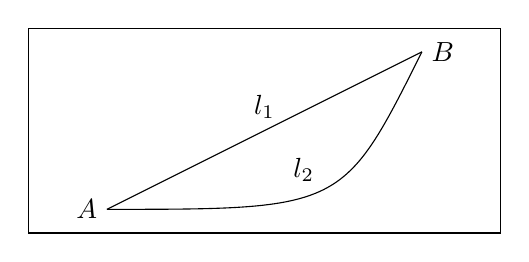
\begin{tikzpicture}[scale=1.0]
                \draw (-3,+1.3) rectangle (+3,-1.3);
                \coordinate (A) at (-2.0,-1);
                \coordinate (B) at (+2,+1);
                \coordinate (C) at (1,-1);

                \draw(A)--(B);
                \draw(A)..controls(C)..(B);

                \node[left] at(A) {$A$};
                \node[right] at(B) {$B$};

                \node at(0,0.3){$l_1$};
                \node at(0.5,-0.5){$l_2$};
            \end{tikzpicture}
            \caption{摩擦力做功示意图}
        \end{center}
    \end{figure}\\
    摩擦力沿$l_1$路径所做的功和摩擦力沿$l_2$路径所做的功是不同的。\\[3mm]
    摩擦力做功的多少与路径有关,摩擦力是一种典型的耗散力。\\[8mm]
    保守力做功的特点可以表示为:
    \begin{large}
        \begin{equation*}
            \oint_L\veb{F}\cdot\dif\veb{s}=0
        \end{equation*}
    \end{large}\\
    耗散力做功的特点可以表示为:
    \begin{large}
        \begin{equation*}
            \oint_L\veb{F}\cdot\dif\veb{s}\neq 0
        \end{equation*}
    \end{large}\\
    即力沿任意闭合路径做功时,保守力所作功总是为零,耗散力所作功总是不为零。

\newpage

\subsubsection{系统的动能定理}
    \setcounter{equation}{0}
    \textbf{系统的动能定理:}系统的外力和内力做功的总和等于系统动能的增量。\\[3mm]
    系统的动能定理的数学表达:
    \begin{large}
        \begin{equation*}
            W_{\text{外}}+W_{\text{内}}=\Delta E_k
        \end{equation*}
    \end{large}\\
    设一个系统中有两个质点,一个称为质点$1$,一个称为质点$2$。\\[3mm]
    质点$1$所受的外力记作$\veb{F_1}$,质点$1$所受的内力记作$\veb{F_1}$。\\[3mm]
    质点$2$所受的外力记作$\veb{F_2}$,质点$2$所受的内力记作$\veb{F_2}$。\\[6mm]
    对质点$1$使用动能定理:
    \begin{equation}
        \int\veb{F_1}\cdot\dif\veb{s_1}+\int\veb{f_1}\cdot\dif\veb{s_1}=\Delta E_{k1}
    \end{equation}\\
    对质点$2$使用动能定理:
    \begin{equation}
        \int\veb{F_2}\cdot\dif\veb{s_2}+\int\veb{f_2}\cdot\dif\veb{s_2}=\Delta E_{k2}
    \end{equation}\\
    由于系统的动能增量能表示为:\vspace{5pt}
    \begin{equation}
        \Delta E_k=\Delta E_{k1}+\Delta E_{k2}
    \end{equation}\\
    由于外力所做的功可以表示为:
    \begin{equation}
        W_{\text{外}}=\int\veb{F_1}\cdot\dif\veb{s_1}+\int\veb{F_2}\cdot\dif\veb{s_2}
    \end{equation}\\
    由于内力所做的功可以表示为:
    \begin{equation}
        W_{\text{内}}=\int\veb{f_1}\cdot\dif\veb{s_1}+\int\veb{f_2}\cdot\dif\veb{s_2}
    \end{equation}\\
    故将两式相加并代入可以得到$W_{\text{外}}+W_{\text{内}}=\Delta E_k$。\\[3mm]
    由此证明了系统的动能定理。

\newpage

\subsubsection{系统的功能原理}
    \setcounter{equation}{0}
    \textbf{系统的功能原理}:系统的外力和耗散内力做功的总和等于系统机械能的增量。\\[3mm]
    系统的功能原理的数学表达:
    \begin{large}
        \begin{equation*}
            W_{\text{外}}+W_{\text{内耗}}=\Delta E
        \end{equation*}
    \end{large}\\
    系统中外力所作的功记作$W_{\text{外}}$。\\[3mm]
    系统中内力所作的功记作$W_{\text{内}}$。\\[3mm]
    系统内力做的功中,由耗散内力完成的功记作$W_{\text{内耗}}$。\\[3mm]
    系统内力做的功中,由保守内力完成的功记作$W_{\text{内保}}$。\\[6mm]
    由系统的动能定理可知:
    \begin{align}
        &\Delta E_k=W_{\text{外}}+W_{\text{内}}\\[3mm]
        &\Delta E_k=W_{\text{外}}+W_{\text{内耗}}+W_{\text{内保}}\\[3mm]
        &\Delta E_k=W_{\text{外}}+W_{\text{内耗}}-\Delta E_p\\[3mm]
        &\Delta W_{\text{外}}+W_{\text{内耗}}=\Delta E_k+\Delta E_p\\[3mm]
        &\Delta W_{\text{外}}+W_{\text{内耗}}=\Delta E
    \end{align}\\
    其中第二步运用了保守了做功的规律$W=-\Delta E_p$。\\[3mm]
    由此证明了系统的功能原理。\\

\subsubsection{机械能守恒定律}
    \textbf{机械能守恒定律:}当一个系统内只有保守力做功时,动能和势能可以互相转化,机械保持不变。\\[3mm]
    机械能守恒定律的数学表达:
    \begin{large}
        \begin{equation*}
            ~~~~\Delta E=0~~~~~~~~(W_{\text{外}}=W_{\text{内耗}}=0)
        \end{equation*}
    \end{large}\\
    机械能守恒定律可以由系统的功能原理直接得到。

\newpage

\section{动量守恒定律}

\subsection{冲量}
    冲量衡量了力在时间上的积累,是一个矢量,通常用符号$\veb{I}$表示,单位是\si{N\cdot s}。\\[3mm]
    冲量的计算公式(恒力的冲量):
    \begin{large}
        \begin{equation*}
            \veb{I}=\veb{F}\cdot t
        \end{equation*}
    \end{large}\\
    冲量的计算公式(变力的冲量):
    \begin{large}
        \begin{equation*}
            \veb{I}=\int_{t_1}^{t_2}\veb{F}\cdot \dif t
        \end{equation*}
    \end{large}\vspace{-10pt}

\subsection{动量}
    动量衡量了物体运动上的强弱,是一个矢量,通常用符号$\veb{P}$表示,单位是\si{kg\cdot m/s}。\\[3mm]
    动量的计算公式:
    \begin{large}
        \begin{equation*}
            \veb{P}=m\cdot\veb{v}
        \end{equation*}
    \end{large}\vspace{-10pt}

\subsubsection{牛顿第二定律的动量形式}
    \textbf{牛顿第二定律的动量形式:}力是动量的变化率,力的方向和动量的方向相同。\\[3mm]
    牛顿第二定律的动量形式的数学表达:
    \begin{large}
        \begin{equation*}
            \veb{F}=\frac{\dif \veb{P}}{\dif t}
        \end{equation*}
    \end{large}\\
    牛顿第二定律的动量形式的推导:
    \setcounter{equation}{0}
    \begin{align}
        \veb{F}
        &=m\cdot\veb{a}\\[3mm]
        &=m\cdot\frac{\dif\veb{v}}{\dif t}\\[3mm]
        &=\frac{\dif}{\dif t}\cdot(m\cdot\veb{v})\\[3mm]
        &=\frac{\dif}{\dif t}\cdot\veb{P}
    \end{align}\\
    由此可见,力即是质量和加速度的乘积,力也是动量关于时间的导数。

\newpage

\subsubsection{动量和冲量的单位}
    动量和冲量的单位是等价的:
    \begin{large}
        \begin{center}
            \si{N\cdot s}~=~\si{kg\cdot m/s}\\[6mm]
        \end{center}
    \end{large}
    这是因为力的单位~\si{N=kg\cdot m/s^2},将其代入左式即可得到这个结论。\\

\subsubsection{动量定理}
    \setcounter{equation}{0}
    \textbf{动量定理:}物体所受外力的冲量等于物体动量的增量。\\[3mm]
    动量定理的数学表达:
    \begin{large}
        \begin{equation*}
            \veb{I}=\veb{P_2}-\veb{P_1}=\veb{\Delta P}
        \end{equation*}
    \end{large}\\
    我们用$P_1$表示时间为$t_1$时的动量。\\[3mm]
    我们用$P_2$表示时间为$t_2$时的动量。\\[3mm]
    由此推导可得:
    \begin{align}
        \veb{I}
        &=\int_{t_1}^{t_2}\veb{F}\cdot\dif t\\[3mm]
        &=\int_{t_1}^{t_2}m\cdot\veb{a}\cdot\dif t\\[3mm]
        &=\int_{\veb{v_1}}^{\veb{v_2}}m\cdot\frac{\dif\veb{v}}{\dif t}\cdot\dif t\\[3mm]
        &=\int_{\veb{v_1}}^{\veb{v_2}}m\cdot\dif\veb{v}\\[3mm]
        &=\int_{\veb{P_1}}^{\veb{P_2}}\dif\veb{P}\\[3mm]
        &=\veb{P_2}-\veb{P_1}\\[3mm]
        &=\Delta\veb{P}
    \end{align}\\
    由此证明了动量定理。

\newpage

\subsubsection{系统的动量定理}
    \setcounter{equation}{0}
    \textbf{系统的动量定理:}系统所受外力的冲量等于系统动量的增量。\\[3mm]
    系统的动量定理的数学表达:
    \begin{large}
        \begin{equation*}
            \veb{I_{\text{外}}}=\veb{\Delta P}
        \end{equation*}
    \end{large}\\
    设一个系统中有两个质点,一个称为质点$1$,一个称为质点$2$。\\[3mm]
    质点$1$所受的外力记作$\veb{F_1}$,质点$1$所受的内力记作$\veb{f_1}$。\\[3mm]
    质点$2$所受的外力记作$\veb{F_2}$,质点$2$所受的内力记作$\veb{f_2}$。\\[6mm]
    对质点$1$使用动量定理:
    \begin{align}
        \int\veb{F_1}\cdot\dif t+\int\veb{f_1}\cdot\dif t=\veb{\Delta P_1}
    \end{align}\\
    对质点$2$使用动量定理:
    \begin{align}
        \int\veb{F_2}\cdot\dif t+\int\veb{f_2}\cdot\dif t=\veb{\Delta P_2}
    \end{align}\\
    由于系统的动量增量可以表示为:
    \begin{align}
        \veb{\Delta P}=\veb{\Delta P_1}+\veb{\Delta P_2}
    \end{align}\\
    由于外力产生的冲量可以表示为:
    \begin{align}
        \veb{I_{\text{外}}}=\int(\veb{F_1}+\veb{F_2})\cdot\dif t
    \end{align}\\
    由于内力产生的冲量可以表示为:
    \begin{align}
        \veb{I_{\text{内}}}=\int(\veb{f_1}+\veb{f_2})\cdot\dif t
    \end{align}\\
    然而根据牛顿第三定律可以发现:
    \begin{align}
        \veb{f_1}+\veb{f_2}=0~~~~\Rightarrow~~~~\veb{I_{\text{内}}}=0
    \end{align}\\
    故将两式相加并代入可以得到$\veb{I_{\text{外}}}=\Delta\veb{P}$。\\[3mm]
    由此证明了系统的动量定理。

\subsubsection{系统的动量守恒定律}
    \setcounter{equation}{0}
    \textbf{系统的动量守恒定律}:系统受到的外力为零时,系统的动量保持不变。\\[3mm]
    系统的动量守恒定律的数学表达:
    \begin{large}
        \begin{equation*}
            ~~~~\veb{\Delta P=0}~~~~~~~~(\veb{F_{\text{外}}}=0)
        \end{equation*}
    \end{large}\\
    由于此时系统受到的外力为零:
    \begin{align}
        \veb{F_{\text{外}}}=0
    \end{align}\\
    所以系统所受外力的冲量为零:
    \begin{align}
        \veb{I_{\text{外}}}=0
    \end{align}\\
    根据动量定义可知$\veb{\Delta P}=\veb{I_{\text{外}}}=0$。\\[3mm]
    由此证明了系统的动量守恒定律。

\newpage

\section{刚体的转动}
    刚体是一种理想模型,当力作用于刚体,只会发生运动状态的改变,不会发生形变。\\[3mm]
    例如研究橡皮在桌面上的运动时,可以将橡皮视为刚体。\\[3mm]
    例如研究橡皮受挤压时的形变时,不能将橡皮视为刚体。

\subsection{刚体的平动和转动}
    刚体最基本的运动可以分为两类:\\[3mm]
    1.刚体的平动,指的是运动时刚体内任一直线的方向都保持不变。\\[3mm]
    2.刚体的转动,指的是运动时刚体内任一质点都绕同一直线转动。\\[5mm]
    下图展示了刚体的平动($\overrightarrow{AB}$方向不变):
    \begin{figure}[h]
        \begin{center}
            \begin{tikzpicture}
                \tkzDefPoint(-3,0){O1}
                \tkzDefPoint(+3,0){O2}

                \tkzDefPoint(-1,0){L1}
                \tkzDefPoint(+1,0){L2}

                \tkzDrawSegment[dashed,-latex](L1,L2)

                \tkzDefShiftPoint[O1](60:1.5){v1}
                \tkzDefShiftPoint[v1](0.8,0){v2}
                \tkzDrawSegment[-latex](v1,v2)
                \tkzLabelPoint[above](v2){$v$}

                \tkzDefShiftPoint[O1](0:1){C1}
                \tkzDefShiftPoint[O1](60:1){B1}
                \tkzDefShiftPoint[O1](120:1){A1}
                \tkzDefShiftPoint[O1](180:1){F1}
                \tkzDefShiftPoint[O1](240:1){E1}
                \tkzDefShiftPoint[O1](300:1){D1}

                \tkzDrawPolygon(A1,B1,C1,D1,E1,F1)
                \tkzDrawSegment[->,very thick](A1,B1)

                \tkzLabelPoint[left=0.2](A1){$A$}
                \tkzLabelPoint[right](B1){$B$}
                \tkzLabelPoint[right](C1){$C$}
                \tkzLabelPoint[right](D1){$D$}
                \tkzLabelPoint[left=0.2](E1){$E$}
                \tkzLabelPoint[left=0.2](F1){$F$}

                \tkzDefShiftPoint[O2](0:1){C2}
                \tkzDefShiftPoint[O2](60:1){B2}
                \tkzDefShiftPoint[O2](120:1){A2}
                \tkzDefShiftPoint[O2](180:1){F2}
                \tkzDefShiftPoint[O2](240:1){E2}
                \tkzDefShiftPoint[O2](300:1){D2}

                \tkzDrawPolygon(A2,B2,C2,D2,E2,F2)
                \tkzDrawSegment[->,very thick](A2,B2)

                \tkzLabelPoint[left=0.2](A2){$A$}
                \tkzLabelPoint[right](B2){$B$}
                \tkzLabelPoint[right](C2){$C$}
                \tkzLabelPoint[right](D2){$D$}
                \tkzLabelPoint[left=0.2](E2){$E$}
                \tkzLabelPoint[left=0.2](F2){$F$}
            \end{tikzpicture}
            \caption{刚体的平动}
        \end{center}
    \end{figure}\\
    下图展示了刚体的转动($\overrightarrow{AB}$方向改变):\vspace{5pt}
    \begin{figure}[h]
        \begin{center}
            \begin{tikzpicture}
                \tkzDefPoint(-3,0){O1}
                \tkzDefPoint(+3,0){O2}

                \tkzDefPoint(-1,0){L1}
                \tkzDefPoint(+1,0){L2}

                \tkzDrawSegment[dashed,-latex](L1,L2)

                \tikzset{compass style/.append style={-latex}}
                \tkzDefShiftPoint[O1](40:1.8){v1}
                \tkzDrawArc[R,color=black](v1,0.35cm)(315,135)
                \tkzLabelPoint[right=0.4](v1){$\omega$}

                \tkzDrawPolygon(A1,B1,C1,D1,E1,F1)
                \tkzDrawSegment[->,very thick](A1,B1)

                \tkzDefShiftPoint[O1](0:1){C1}
                \tkzDefShiftPoint[O1](60:1){B1}
                \tkzDefShiftPoint[O1](120:1){A1}
                \tkzDefShiftPoint[O1](180:1){F1}
                \tkzDefShiftPoint[O1](240:1){E1}
                \tkzDefShiftPoint[O1](300:1){D1}

                \tkzLabelPoint[left=0.2](A1){$A$}
                \tkzLabelPoint[right](B1){$B$}
                \tkzLabelPoint[right](C1){$C$}
                \tkzLabelPoint[right](D1){$D$}
                \tkzLabelPoint[left=0.2](E1){$E$}
                \tkzLabelPoint[left=0.2](F1){$F$}

                \tkzDefShiftPoint[O2](0:1){D2}
                \tkzDefShiftPoint[O2](60:1){C2}
                \tkzDefShiftPoint[O2](120:1){B2}
                \tkzDefShiftPoint[O2](180:1){A2}
                \tkzDefShiftPoint[O2](240:1){F2}
                \tkzDefShiftPoint[O2](300:1){E2}

                \tkzDrawPolygon(A2,B2,C2,D2,E2,F2)
                \tkzDrawSegment[->,very thick](A2,B2)

                \tkzLabelPoint[left=0.2](A2){$A$}
                \tkzLabelPoint[left=0.2](B2){$B$}
                \tkzLabelPoint[right](C2){$C$}
                \tkzLabelPoint[right](D2){$D$}
                \tkzLabelPoint[right](E2){$E$}
                \tkzLabelPoint[left=0.2](F2){$F$}
            \end{tikzpicture}
            \caption{刚体的转动}
        \end{center}
    \end{figure}\\
    刚体的转动中所绕的直线称为转轴,若转轴位置保持不变,则称为定轴转动。\\[3mm]
    刚体的一般运动可以视为平动和转动的叠加。

\newpage

\subsection{力矩}
    力矩衡量了力对刚体的转动作用,是一个矢量,通常用符号$\veb{M}$表示,单位是\si{N\cdot m}。\\[3mm]
    力矩可以用转轴到力的作用线的距离$d$表示:
    \begin{large}
        \begin{equation*}
            M=F\cdot d
        \end{equation*}
    \end{large}\\
    力矩可以用转轴到力的作用点的距离$r$表示:
    \begin{large}
        \begin{equation*}
            M=F\cdot r\cdot\sin{\varphi}
        \end{equation*}
    \end{large}\\
    力矩的示意图如下:
    \begin{figure}[h]
        \begin{center}
            \begin{tikzpicture}
                \draw (0,0) ellipse (4 and 2);
                \draw[dashed] (0,0) ellipse (2 and 1);
        
                \tkzDefPoint(0,0){O}
                \tkzDefPoint(2,0){A}
                \tkzDefPoint(4,0){B}
                \tkzDefShiftPoint[A](35:1.3){C}
                \tkzDefShiftPoint[A](215:1){D}

                \tkzDefPoint(0,+4){M1}
                \tkzDefPoint(0,-2){M2}
                \tkzDefPoint(0,-4){M3}

                \tkzDrawSegment[-latex](O,M1)
                \tkzDrawSegment[dashed](O,M2)
                \tkzDrawSegment[solid](M2,M3)

                \tkzDrawSegment[-latex,solid](O,A)
                \tkzDrawSegment[dashed](A,B)

                \tkzDrawSegment[-latex,solid](A,C)
                \tkzDrawSegment[dashed](A,D)
                \tkzDrawSegment[solid](O,D)

                \tkzMarkRightAngle[size=0.15](O,D,A)
                \tkzMarkAngle[size=0.311](B,A,C)

                \tkzDefShiftPoint[A](0.4,0.4){phi}
                \tkzLabelPoint(phi){$\varphi$}
                \tkzLabelPoint[above left](C){$\veb{F}$}
                \tkzLabelSegment[above](O,A){$\veb{r}$}
                \tkzLabelSegment[below](O,D){$h$}

                \tkzDefPoint(20:4){V}
                \tikzset{compass style/.append style={-latex}}
                \tkzDrawArc[R,color=black](V,0.35cm)(315,135)
                \tkzLabelPoint[right=0.4](V){$\omega$}

                \tkzLabelPoint[right](M1){$\veb{M}$}
            \end{tikzpicture}
            \caption{力矩的示意图}
        \end{center}
    \end{figure}\\
    其中转轴到力的作用线的距离$d$称为力臂。\\[3mm]
    力矩是矢量,其方向为右手四指沿位矢$\veb{r}$的方向至力$\veb{F}$的方向螺旋时右手拇指指向的方向。\\[6mm]
    力矩的计算公式:
    \begin{large}
        \begin{equation*}
            \veb{M}=\veb{r}\times\veb{F}
        \end{equation*}
    \end{large}\\
    力矩在定轴转动中,方向总是沿着转轴方向。

\subsubsection{转动定律}
    \setcounter{equation}{0}
    \textbf{转动定律:}当力矩作用于刚体时,刚体所得到的角加速度的大小,与刚体所受的合力矩成正比,
    与刚体的转动惯量成反比,刚体角加速度的方向与刚体所受的合力矩方向相同。\\[3mm]
    转动定律的数学表达:
    \begin{large}
        \begin{equation*}
            \veb{M}=J\cdot\veb{\alpha}
        \end{equation*}
    \end{large}\\
    考虑刚体中的一个质点$P_i$:\\[3mm]
    1.质点$P_i$所受合外力在转动平面内的分量为$F_i$,其与位矢所成角度为$\varphi_i$。\\[3mm]
    2.质点$P_i$所受合内力在转动平面内的分量为$f_i\,$,其与位矢所成角度为$\beta_i$。\\[3mm]
    \begin{figure}[h]
        \begin{center}
            \begin{tikzpicture}[scale=0.7]
                \tkzDefPoint(0,0){O}
                \tkzDrawCircle[R](O,4cm)

                \tkzDefPoint(3,0){P}
                \tkzDefShiftPoint[P](135:2){f}
                \tkzDefShiftPoint[P](90:2){F}

                \tkzDrawSegment(O,P)
                \tkzDrawSegment[-latex](P,f)
                \tkzDrawSegment[-latex](P,F)

                \tkzMarkAngle[size=0.500](f,P,O)
                \tkzMarkAngle[size=0.311](F,P,O)

                \tkzDefShiftPoint[P](-0.7,1.0){p}
                \tkzDefShiftPoint[P](-1.2,0.75){b}

                \tkzLabelPoint(p){$\varphi_i$}
                \tkzLabelPoint(b){$\beta_i$}

                \tkzLabelPoint[below](O){$O$}
                \tkzLabelPoint[below](P){$P_i$}
                \tkzLabelPoint[left](f){$f_i$}
                \tkzLabelPoint[left](F){$F_i$}
                \tkzLabelSegment[below](O,P){$r_i$}
            \end{tikzpicture}
            \caption{质点$P_i$的受力示意图}
        \end{center}
    \end{figure}\\
    将力分解为法向分量:
    \begin{align}
        F_i\cdot\cos\varphi_i+f_i\cdot\cos\beta_i=m_i\cdot a_{ni}=m_i\cdot r_i\cdot\omega^2
    \end{align}\\
    将力分解为切向分量:
    \begin{align}
        F_i\cdot\sin\varphi_i+f_i\cdot\sin\beta_i=m_i\cdot a_{ti}=m_i\cdot r_i\cdot\alpha
    \end{align}\\
    对于法向分量,其通过转轴,力矩为零不予考虑。\\[3mm]
    对于切向分量,将两边同乘$r_i$可得:
    \begin{align}
        F_i\cdot r_i\cdot\sin\varphi_i+f_i\cdot r_i\cdot\sin\beta_i=m_i\cdot r_i^2\cdot\alpha
    \end{align}

\newpage

    考虑所有质点则有:
    \begin{align}
        \sum F_i\cdot r_i\cdot\sin\varphi_i+\sum f_i\cdot r_i\cdot\sin\beta_i=\left(\sum m_i\cdot r_i^2\right)\cdot\alpha
    \end{align}\\
    其中第一项表示合外力的力矩:
    \begin{align}
        \sum F_i\cdot r_i\cdot\sin\varphi_i
    \end{align}\\
    其中第二项表示合内力的力矩:
    \begin{align}
        \sum f_i\cdot r_i\cdot\sin\beta_i
    \end{align}\\
    根据牛顿第三定律,合内力中的作用力和反作用力相互抵消,故内力的合力矩为零。\\[16mm]
    因此可以得到:
    \begin{align}
        \sum F_i\cdot r_i\cdot\sin\varphi_i=\left(\sum m_i\cdot r_i^2\right)\cdot\alpha
    \end{align}\\
    定义力矩$M$为:
    \begin{align}
        M=\sum F_i\cdot r_i\cdot\sin\varphi_i
    \end{align}\\
    定义转动惯量$J$为:
    \begin{align}
        J=\sum m_i\cdot r_i^2
    \end{align}\\
    将其代入可得:
    \begin{align}
        \veb{M}=J\cdot\veb{\alpha}
    \end{align}\\
    由此证明了转动定律。

\newpage

\subsubsection{转动惯量}
    转动惯量衡量了刚体保持原有转动状态的惯性,是一个标量,通常用符号$J$表示,单位是\si{kg\cdot m^2}。\\[3mm]
    转动惯量的计算公式(质量离散分布):
    \begin{large}
        \begin{equation*}
            J=\sum m_i\cdot r_i^2
        \end{equation*}
    \end{large}\\
    转动惯量的计算公式(质量连续分布):
    \begin{large}
        \begin{equation*}
            J=\int r^2\cdot\dif m~
        \end{equation*}
    \end{large}

\subsubsection{细棒的转动惯量}
    细棒的转动惯量(转轴过中心且垂直):
    \begin{large}
        \begin{equation*}
            J=\frac{1}{12}\cdot m\cdot L^2    
        \end{equation*}
    \end{large}\\
    细棒的转动惯量(转轴过一端且垂直):
    \begin{large}
        \begin{equation*}
            J=\frac{1}{3}\cdot m\cdot L^2    
        \end{equation*}
    \end{large}\\
    细棒的示意图如下:
    \begin{figure}[h]
        \begin{center}
            \subfigure[转轴过中心]
            {
                \begin{tikzpicture}
                    \tkzDefPoint(+2.5,+0.2){A}
                    \tkzDefPoint(+2.5,-0.2){B}
                    \tkzDefPoint(-2.5,+0.2){C}
                    \tkzDefPoint(-2.5,-0.2){D}

                    \tkzDrawPolygon(A,B,D,C)

                    \tkzDefShiftPoint[B](0,-0.2){E}
                    \tkzDefShiftPoint[D](0,-0.2){F}

                    \tkzDrawSegment[thin](B,E)
                    \tkzDrawSegment[thin](D,F)

                    \tkzDefMidPoint(B,E)
                    \tkzGetPoint{M}
                    \tkzDefMidPoint(D,F)
                    \tkzGetPoint{N}

                    \tkzDrawSegment[<->](M,N)
                    \tkzLabelSegment[below,pos=0.25](M,N){$L$}

                    \tkzDefMidPoint(A,C)
                    \tkzGetPoint{Z1}

                    \tkzDefMidPoint(B,D)
                    \tkzGetPoint{Z2}

                    \tkzDefShiftPoint[Z1](0,-2){Z3}
                    \tkzDefShiftPoint[Z2](0,+2){Z4}

                    \tkzDrawSegment(Z3,Z4)

                    \tkzLabelPoint[right](Z4){转轴}
                \end{tikzpicture}
            }\qquad\qquad\qquad
            \subfigure[转轴过中心]
            {
                \begin{tikzpicture}
                    \tkzDefPoint(+2.5,+0.2){A}
                    \tkzDefPoint(+2.5,-0.2){B}
                    \tkzDefPoint(-2.5,+0.2){C}
                    \tkzDefPoint(-2.5,-0.2){D}

                    \tkzDrawPolygon(A,B,D,C)

                    \tkzDefShiftPoint[B](0,-0.2){E}
                    \tkzDefShiftPoint[D](0,-0.2){F}

                    \tkzDrawSegment[thin](B,E)
                    \tkzDrawSegment[thin](D,F)

                    \tkzDefMidPoint(B,E)
                    \tkzGetPoint{M}
                    \tkzDefMidPoint(D,F)
                    \tkzGetPoint{N}

                    \tkzDrawSegment[<->](M,N)
                    \tkzLabelSegment[below,pos=0.5](M,N){$L$}

                    \tkzDefShiftPoint[A](0,-2){Z3}
                    \tkzDefShiftPoint[B](0,+2){Z4}

                    \tkzDrawSegment(Z3,Z4)

                    \tkzLabelPoint[left](Z4){转轴}
                \end{tikzpicture}
            }
            \caption{细棒的示意图}
        \end{center}
    \end{figure}\\
    上述公式中,符号$m$表示棒的质量,符号$L$表示棒的长度。

\newpage

    在距转轴$x$处取长度元$\dif x$,其质量为$\dif m$,设棒质量的线密度为$\lambda$。\\[3mm]
    显然有以下关系式:
    \setcounter{equation}{0}
    \begin{align}
        \dif m=\lambda\cdot\dif x
    \end{align}\\
    线密度可以表示为:
    \begin{align}
        \lambda=\frac{m}{L}
    \end{align}\\
    当转轴过中心时有:
    \begin{align}
        J
        &=\int_{-\frac{L}{2}}^{+\frac{L}{2}}x^2\cdot\dif m\\[3mm]
        &=\int_{-\frac{L}{2}}^{+\frac{L}{2}}x^2\cdot\lambda\cdot\dif x\\[3mm]
        &=\lambda\cdot\int_{-\frac{L}{2}}^{+\frac{L}{2}}x^2\cdot\dif x\\[3mm]
        &=\lambda\cdot\left[\frac{1}{3}\cdot x^3\right]_{-\frac{L}{2}}^{+\frac{L}{2}}\\[3mm]
        &=\lambda\cdot\frac{L^3}{12}\\[3mm]
        &=\frac{1}{12}\cdot\lambda\cdot L^3\\[3mm]
        &=\frac{1}{12}\cdot\frac{m}{L}\cdot L^3\\[3mm]
        &=\frac{1}{12}\cdot m\cdot L^3
    \end{align}\\
    由此证明了转轴过中心时的转动惯量。

\newpage

    在距转轴$x$处取长度元$\dif x$,其质量为$\dif m$,设棒质量的线密度为$\lambda$。\\[3mm]
    显然有以下关系式:
    \setcounter{equation}{0}
    \begin{align}
        \dif m=\lambda\cdot\dif x
    \end{align}\\
    线密度可以表示为:
    \begin{align}
        \lambda=\frac{m}{L}
    \end{align}\\
    当转轴过一端时有:
    \begin{align}
        J
        &=\int_{0}^{L}x^2\cdot\dif m\\[3mm]
        &=\int_{0}^{L}x^2\cdot\lambda\cdot\dif x\\[3mm]
        &=\lambda\cdot\int_{0}^{L}x^2\cdot\dif x\\[3mm]
        &=\lambda\cdot\left[\frac{1}{3}\cdot x^3\right]_{0}^{L}\\[3mm]
        &=\lambda\cdot\frac{L^3}{3}\\[3mm]
        &=\frac{1}{3}\cdot\lambda\cdot L^3\\[3mm]
        &=\frac{1}{3}\cdot\frac{m}{L}\cdot L^3\\[3mm]
        &=\frac{1}{3}\cdot m\cdot L^3
    \end{align}\\
    由此证明了转轴过一端时的转动惯量。

\newpage

\subsubsection{圆盘的转动惯量}
    圆盘的转动惯量:
    \begin{large}
        \begin{equation*}
            J=\frac{1}{2}\cdot m\cdot R^2
        \end{equation*}
    \end{large}\\
    圆盘的示意图如下:
    \begin{figure}[h]
        \begin{center}
            \begin{tikzpicture}[scale=0.8]
                \draw (0,0) ellipse(4 and 2);

                \tkzDefPoint(0,0){O}

                \tkzDefPoint(0,+6){M1}
                \tkzDefPoint(0,-2){M2}
                \tkzDefPoint(0,-6){M3}

                \tkzDrawSegment(O,M1)
                \tkzDrawSegment[dashed](O,M2)
                \tkzDrawSegment(M2,M3)

                \tkzLabelPoint[right](M1){转轴}

                \tkzDefPoint(4,0){R}

                \tkzDrawSegment(O,R)
                \tkzLabelSegment[above](O,R){$R$}
            \end{tikzpicture}
            \caption{圆盘的示意图}
        \end{center}
    \end{figure}\\
    上述公式中,符号$m$表示圆盘的质量,符号$L$表示圆盘的半径。

\newpage

    在距离转轴$r$处取一薄圆环,其宽度为$\dif r$,其质量为$\dif m$,设圆盘的面密度为$\sigma$。\\[3mm]
    显然有以下关系式:
    \setcounter{equation}{0}
    \begin{align}
        \dif m=2\cdot\pi\cdot r\cdot\sigma\cdot\dif r
    \end{align}\\
    面密度可以表示为:
    \begin{align}
        \sigma=\frac{m}{\pi\cdot R^2}
    \end{align}\\
    推导圆盘的转动惯量:
    \begin{align}
        J
        &=\int_{0}^{R} r^2\cdot\dif m\\[3mm]
        &=\int_{0}^{R} r^2\cdot 2\cdot\pi\cdot r\cdot\sigma\cdot\dif r\\[3mm]
        &=\int_{0}^{R} 2\cdot\pi\cdot r^3\cdot\sigma\cdot\dif r\\[3mm]
        &=2\cdot\pi\cdot\sigma\cdot\int_{0}^{R}r^3\cdot\dif r\\[3mm]
        &=2\cdot\pi\cdot\sigma\cdot\left[\frac{1}{4}\cdot r^4\right]_{0}^{R}\\[3mm]
        &=\frac{1}{2}\cdot\pi\cdot\sigma\cdot R^4\\[3mm]
        &=\frac{1}{2}\cdot\pi\cdot R^4\cdot\frac{m}{\pi\cdot R^2}\\[3mm]
        &=\frac{1}{2}\cdot m\cdot R^2
    \end{align}\\
    由此证明了圆盘的转动惯量。

\newpage

\subsubsection{圆环的转动惯量}
    圆环的转动惯量:
    \begin{large}
        \begin{equation*}
            J=\frac{1}{2}\cdot m\cdot\left[R_1^2+R_2^2\right]
        \end{equation*}
    \end{large}\\
    圆环的示意图如下:
    \begin{figure}[h]
        \begin{center}
            \begin{tikzpicture}[scale=0.8]
                \draw (0,0) ellipse(4 and 2);
                \draw (0,0) ellipse(2 and 1);

                \tkzDefPoint(0,0){O}

                \tkzDefPoint(0,+6){M1}
                \tkzDefPoint(0,-1){M2}
                \tkzDefPoint(0,-2){M3}
                \tkzDefPoint(0,-6){M4}

                \tkzDrawSegment(M1,M2)
                \tkzDrawSegment[dashed](M2,M3)
                \tkzDrawSegment(M3,M4)

                \tkzLabelPoint[right](M1){转轴}

                \tkzDefPoint(2,0){R1}
                \tkzDefPoint(2,-1.732){R2}

                \tkzDrawSegment(O,R1)
                \tkzDrawSegment(O,R2)
                \tkzLabelSegment[above](O,R1){$R_1$}
                \tkzLabelSegment[above right,pos=0.75](O,R2){$R_2$}
            \end{tikzpicture}
            \caption{圆盘的示意图}
        \end{center}
    \end{figure}\\
    上述公式中,符号$m$表示圆盘的质量,符号$L$表示圆盘的半径。

\newpage

    在距离转轴$r$处取一薄圆环,其宽度为$\dif r$,其质量为$\dif m$,设圆盘的面密度为$\sigma$。\\[3mm]
    显然有以下关系式:
    \setcounter{equation}{0}
    \begin{align}
        \dif m=2\cdot\pi\cdot r\cdot\sigma\cdot\dif r
    \end{align}\\
    面密度可以表示为:
    \begin{align}
        \sigma=\frac{m}{\pi\cdot\left[R_2^2-R_1^2\right]}
    \end{align}\\
    推导圆环的转动惯量:
    \begin{align}
        ~~~~~~~~~~~~J
        &=\int_{R_1}^{R_2} r^2\cdot\dif m\\[3mm]
        &=\int_{R_1}^{R_2} r^2\cdot 2\cdot\pi\cdot r\cdot\sigma\cdot\dif r\\[3mm]
        &=\int_{R_1}^{R_2} 2\cdot\pi\cdot r^3\cdot\sigma\cdot\dif r\\[3mm]
        &=2\cdot\pi\cdot\sigma\cdot\int_{R_1}^{R_2}r^3\cdot\dif r\\[3mm]
        &=2\cdot\pi\cdot\sigma\cdot\left[\frac{1}{4}\cdot r^4\right]_{R_1}^{R_2}\\[3mm]
        &=\frac{1}{2}\cdot\pi\cdot\sigma\cdot\left[R_2^4-R_1^4\right]\\[3mm]
        &=\frac{1}{2}\cdot\pi\cdot\sigma\cdot\left[R_2^2+R_1^2\right]\cdot\left[R_2^2+R_1^2\right]\\[3mm]
        &=\frac{1}{2}\cdot\pi\cdot\frac{m}{\pi\cdot\left[R_2^2-R_1^2\right]}\cdot\left[R_2^2-R_1^2\right]\cdot\left[R_2^2+R_1^2\right]\\[3mm]
        &=\frac{1}{2}\cdot m\cdot\left[R_1^2+R_2^2\right]
    \end{align}\\
    由此证明了圆环的转动惯量。

\newpage

\subsection{力矩的功}
    力矩的功衡量了力矩在空间上的积累,是一个标量,通常用符号$W$表示,单位是\si{J}。\\[3mm]
    力矩的功的计算公式(恒力矩做功):
    \begin{large}
        \begin{equation*}
            W=M\cdot\theta
        \end{equation*}
    \end{large}\\
    力矩的功的计算公式(变力矩做功):
    \begin{large}
        \begin{equation*}
            W=\int_{\theta_1}^{\theta_2} M\cdot\dif\theta
        \end{equation*}
    \end{large}\\
    力矩的功率衡量了力矩做功的快慢,是一个标量,通常用符号$P$表示,单位是\si{W}。\\[3mm]
    力矩的功率的计算公式:
    \begin{large}
        \begin{equation*}
            P=M\cdot\omega
        \end{equation*}
    \end{large}\\
    力矩的功和功率的示意图如下:
    \begin{figure}[h]
        \begin{center}
            \begin{tikzpicture}[scale=1.0]
                \draw (0,0) ellipse(4 and 2);
                \draw[dashed] (0,0) ellipse(2 and 1);

                \tkzDefPoint(0,0){O}

                \tkzDefPoint(0,+4){M1}
                \tkzDefPoint(0,-2){M2}
                \tkzDefPoint(0,-4){M3}

                \tkzDrawSegment[-latex](O,M1)
                \tkzDrawSegment[dashed](M1,M2)
                \tkzDrawSegment(M2,M3)

                \tkzLabelPoint[right](M1){$M$}

                \tkzDefPoint(2,0){A}
                \tkzDefPoint(4,0){B}
                \tkzDefPoint(1,0.866){C}
                \tkzDefShiftPoint[A](35:1.3){F}

                \tkzDrawSegment[-latex](O,A)
                \tkzDrawSegment(O,C)
                \tkzDrawSegment[dashed](A,B)
                \tkzDrawSegment[-latex](A,F)
                \tkzDrawSegment[-latex](A,C)

                \tkzMarkAngle[size=0.311](A,O,C)
                \tkzMarkAngle[size=0.311](B,A,F)
                \tkzMarkAngle[size=0.224](F,A,C)

                \tkzDefShiftPoint[O](0.3,0.5){theta}
                \tkzLabelPoint(theta){$\dif\theta$}

                \tkzDefShiftPoint[A](0.25,0.35){alpha}
                \tkzLabelPoint(alpha){$\alpha$}

                \tkzDefShiftPoint[A](-0.1,0.7){beta}
                \tkzLabelPoint(beta){$\beta$}

                \tkzLabelPoint[right](F){$\veb{F}$}

                \tkzLabelSegment[below](O,A){$\veb{r}$}
                \tkzLabelSegment[above right,pos=0.7](A,C){$\veb{\dif s}$}

                \tkzDefPoint(20:4){V}
                \tikzset{compass style/.append style={-latex}}
                \tkzDrawArc[R,color=black](V,0.35cm)(315,135)
                \tkzLabelPoint[right=0.4](V){$\omega$}
            \end{tikzpicture}
            \caption{力矩的功和功率的示意图}
        \end{center}
    \end{figure}\\
    其中角$\alpha$为力$\veb{F}$和位矢$\veb{r}$的夹角。\\[3mm]
    其中角$\beta$为力$\veb{F}$和位矢$\veb{r}$的夹角。\\[3mm]
    由于$\dif\theta$很小,所以实际上$\alpha+\beta=90^\circ$。

\newpage

    由于力$\veb{F}$在位移$\dif s$中所作的功为:
    \setcounter{equation}{0}
    \begin{align}
        \dif W
        &=F\cdot\dif s\cdot\cos{\beta}\\[3mm]
        &=F\cdot\dif s\cdot\sin{\alpha}\\[3mm]
        &=F\cdot r\cdot\dif\theta\cdot\sin{\alpha}\\[3mm]
        &=F\cdot r\cdot\sin{\alpha}\cdot\dif\theta\\[3mm]
        &=M\cdot\dif\theta
    \end{align}\\
    因为力矩$M$在角位移由$\theta_1$至$\theta_2$中所做的功为:\vspace{3pt}
    \begin{align}
        W
        &=\int_{\theta_1}^{\theta_2}\dif W\\[3mm]
        &=\int_{\theta_1}^{\theta_2}M\cdot\dif\theta~~~~~~~~~
    \end{align}\\
    因为力矩$M$的功率$P$为功$W$对时间$t$的导数:\vspace{5pt}
    \begin{align}
        P
        &=\frac{\dif W}{\dif t}\\[3mm]
        &=\frac{\dif}{\dif t}\cdot\int M\cdot\dif\theta\\[3mm]
        &=\frac{\dif}{\dif t}\cdot\int M\cdot\omega\cdot\dif t\\[3mm]
        &=M\cdot\omega
    \end{align}\\
    由此证明了力矩的功和功率的计算公式。

\newpage

\subsection{转动动能}
    \setcounter{equation}{0}
    转动动能衡量了刚体由于转动而具有的能量,是一个标量,通常用符号$E_k$表示,单位是\si{J}。\\[3mm]
    转动动能定义为刚体从角速度为$0$时至角速度为$\omega$时,外力矩所做的功。\\[3mm]
    转动动能的计算公式:
    \begin{large}
        \begin{equation*}
            E_k=\frac{1}{2}\cdot J\cdot\omega^2
        \end{equation*}
    \end{large}\\
    由变力矩做功的计算公式机进行推导:
    \begin{align}
        W
        &=\int_{\theta_1}^{\theta_2}M\cdot\dif\theta\\[3mm]
        &=\int_{t_1}^{t_2}M\cdot\omega\cdot\dif t\\[3mm]
        &=\int_{t_1}^{t_2}J\cdot\alpha\cdot\omega\cdot\dif t\\[3mm]
        &=\int_{\omega_1}^{\omega_2}J\cdot\frac{\dif\omega}{\dif t}\cdot\omega\cdot\dif t\\[3mm]
        &=\int_{\omega_1}^{\omega_2}J\cdot\omega\cdot\dif\omega\\[3mm]
        &=\frac{1}{2}\cdot J\cdot\omega_2^2-\frac{1}{2}\cdot J\cdot\omega_1^2
    \end{align}\\
    根据转动动能定义,初角速度为$\omega_1=0$,末角速度为$\omega_2=\omega$,代入即可得到转动动能的公式。

\newpage

\subsubsection{转动的动能定理}
    \textbf{转动的动能定理:}外力矩对刚体所做的功等于刚体转动动能的增量。\\[3mm]
    转动的动能定理的数学表达:
    \begin{large}
        \begin{equation*}
            W=E_{k_2}-E_{k_1}=\Delta E_k
        \end{equation*}
    \end{large}\\
    我们用$E_{k_1}$表示角速度为$\omega_1$时的转动动能。\\[3mm]
    我们用$E_{k_2}$表示角速度为$\omega_2$时的转动动能。\\[3mm]
    由此推导可得:
    \setcounter{equation}{0}
    \begin{align}
        W
        &=\int_{\theta_1}^{\theta_2}M\cdot\dif\theta\\[3mm]
        &=\int_{t_1}^{t_2}M\cdot\omega\cdot\dif t\\[3mm]
        &=\int_{t_1}^{t_2}J\cdot\alpha\cdot\omega\cdot\dif t\\[3mm]
        &=\int_{\omega_1}^{\omega_2}J\cdot\frac{\dif\omega}{\dif t}\cdot\omega\cdot\dif t\\[3mm]
        &=\int_{\omega_1}^{\omega_2}J\cdot\omega\cdot\dif\omega\\[3mm]
        &=E_{k2}-E_{k1}\\[3mm]
        &=\Delta E_k
    \end{align}\\
    由此证明了转动的动能定理。

\newpage

\section{角动量守恒定律}

\subsection{角冲量}
    角冲量衡量了力矩在时间上的积累,是一个矢量,通常用符号$\veb{H}$表示,单位是\si{N\cdot s^2}。\\[3mm]
    角冲量的计算公式(恒力矩的冲量):
    \begin{large}
        \begin{equation*}
            \veb{H}=\veb{M}\cdot t
        \end{equation*}
    \end{large}\\
    角冲量的计算公式(变力矩的冲量):
    \begin{large}
        \begin{equation*}
            \veb{H}=\int_{t_1}^{t_2}\veb{M}\cdot\dif t
        \end{equation*}
    \end{large}

\subsection{角动量}
    角动量衡量了物体在转动上的强弱,是一个矢量,通常用符号$\veb{L}$表示,单位是\si{kg\cdot m}。\\[3mm]
    角动量的计算公式:
    \begin{large}
        \begin{align*}
            &\veb{L}=\veb{r}\times\veb{v}\cdot m\\[3mm]
            &\veb{L}=\veb{r}\times\veb{p}
        \end{align*}
    \end{large}\\
    角动量大小的计算公式:
    \begin{large}
        \begin{align*}
            &L=r\cdot m\cdot v\cdot\sin{\theta}\\[3mm]
            &L=r\cdot p\cdot\sin{\theta}
        \end{align*}
    \end{large}\\
    其中$\theta$可以是位矢$\veb{r}$与速度$\veb{v}$所成的角。\\[3mm]
    其中$\theta$可以是位矢$\veb{r}$与动量$\veb{p}$所成的角。\\[3mm]
    其中$\veb{r}$是质点相较于某一参考点的位矢,该参考点可以根据情况任意选择。\\[3mm]
    因此讨论质点的角动量时,必须指明是对于哪一参考点的角动量。

\newpage

\subsubsection{角动量和角冲量的单位}
    角动量和角冲量的单位是等价的:
    \begin{large}
        \begin{center}
            \si{N\cdot s^2}~=~\si{kg\cdot m}\\[6mm]
        \end{center}
    \end{large}
    这是因为力的单位~\si{N=kg\cdot m/s^2},将其代入左式即可得到这个结论。\\

\subsubsection{角动量定理}
    \textbf{角动量定理:}物体所受合力矩的角冲量等于物体角动量的增量。\\[3mm]
    角动量定理的数学表达:
    \begin{large}
        \begin{equation*}
            \veb{H}=\veb{L_2}-\veb{L_1}=\veb{\Delta L}
        \end{equation*}
    \end{large}\\
    我们用$\veb{L_1}$表示时间为$t_1$时的角动量。\\[3mm]
    我们用$\veb{L_2}$表示时间为$t_2$时的角动量。\\[3mm]
    由此推导可得:
    \setcounter{equation}{0}
    \begin{align}
        \veb{H}
        &=\int_{t_1}^{t_2}\veb{M}\cdot\dif t\\[3mm]
        &=\int_{t_1}^{t_2}\veb{r}\times\veb{F}\cdot\dif t\\[3mm]
        &=\veb{r}\times\int_{t_1}^{t_2}m\cdot\veb{a}\cdot\dif t\\[3mm]
        &=\veb{r}\times\int_{t_1}^{t_2}m\cdot\frac{\dif\veb{v}}{\dif t}\cdot\dif t\\[3mm]
        &=\veb{r}\times\int_{t_1}^{t_2}m\cdot\dif\veb{v}\\[3mm]
        &=\veb{r}\times\int_{\veb{p_1}}^{\veb{p_2}}m\cdot\dif\veb{p}\\[3mm]
        &=\veb{r}\times(\veb{p_2}-\veb{p_1})\\[3mm]
        &=\veb{L_2}-\veb{L_1}\\[3mm]
        &=\veb{\Delta L}
    \end{align}\\
    由此证明了角动量定理。

\newpage

\subsubsection{角动量守恒定律}
    \textbf{角动量守恒定律:}物体所受力矩为零时,物体的角动量保持不变。\\[3mm]
    角动量守恒定律的数学表达:
    \begin{large}
        \begin{equation*}
            \veb{\Delta L}=0~~~~(\veb{M}=0)
        \end{equation*}
    \end{large}\\
    由于此时物体受到的力矩为零:
    \begin{large}
        \begin{equation*}
            \veb{M}=0
        \end{equation*}
    \end{large}\\
    故物体所受力矩的角冲量为零:
    \begin{large}
        \begin{equation*}
            \veb{H}=0
        \end{equation*}
    \end{large}\\
    根据角动量定理可知$\veb{\Delta L}=\veb{H}=0$。\\[3mm]
    由此证明了角动量守恒定律。\\[8mm]
    质点的角动量守恒有两种情况:\\[3mm]
    1.质点所受力$\veb{F}=0$,致使力矩$\veb{M}=0$。\\[3mm]
    2.质点所受力$\veb{F}\neq 0$,但力$\veb{F}$指向参考点,致使力矩$\veb{M}=0$。\\[4mm]
    因此如果作用于质点的力是有心力,那么该质点以力心作为参考点的角动量守恒。\\[3mm]
    例如行星绕太阳以椭圆轨道运行时,以及彗星绕太阳以双曲线轨道运行时,引力始终指向太阳,
    故引力是一个有心力,且引力的力心是太阳,因此以太阳为参考点时行星和彗星的角动量守恒。

\newpage

\subsection{刚体定轴转动的角动量}
    \setcounter{equation}{0}
    刚体定轴转动的角动量:
    \begin{large}
        \begin{equation*}
            \veb{L}=J\cdot\veb{\omega}
        \end{equation*}
    \end{large}\\
    考虑一个定轴转动的刚体,以角速度$\veb{\omega}$转动。\\[3mm]
    刚体上一质点对轴的角动量为:
    \begin{align}
        &L_i=r_i\cdot m_i\cdot v\\[3mm]
        &L_i=r_i^2\cdot m_i\cdot\omega
    \end{align}\\
    刚体整体对轴的角动量为:
    \begin{align}
        &L=\sum r_i^2\cdot m_i\cdot\omega\\[3mm]
        &L=\sum\left(r_i^2\cdot m_i\right)\cdot\omega\\[3mm]
        &L=\sum\left(m_i\cdot r_i^2\right)\cdot\omega\\[3mm]
        &L=J\cdot\veb{\omega}
    \end{align}

\subsubsection{转动定律的角动量形式}
    \textbf{转动定律的角动量形式:}力矩是角动量的变化率,力矩的方向和角动量的方向相同。\\[3mm]
    转动定律的角动量形式的数学表达:
    \begin{large}
        \begin{equation*}
            \veb{M}=\frac{\dif L}{\dif t}
        \end{equation*}
    \end{large}\\
    转动定律的角动量形式的推导:
    \begin{align}
        \veb{M}
        &=J\cdot\veb{\alpha}\\[3mm]
        &=J\cdot\frac{\dif\veb{\omega}}{\dif t}\\[3mm]
        &=\frac{\dif}{\dif t}\cdot(J\cdot\veb{\omega})\\[3mm]
        &=\frac{\dif}{\dif t}\cdot\veb{L}
    \end{align}\\
    由此可见,力矩即是转动惯量和角加速度的乘积,力矩也是角动量关于时间的导数。

\newpage

\subsubsection{刚体定轴转动的角动量定理}
    \setcounter{equation}{0}
    \textbf{刚体定轴转动的角动量定理:}刚体所受合外力矩的角冲量等于刚体角动量的增量。\\[3mm]
    刚体定轴转动的角动量定理的数学表达:
    \begin{large}
        \begin{equation*}
            \veb{H_{\text{外}}}=\veb{\Delta L}
        \end{equation*}
    \end{large}\\
    我们用$\veb{L_1}$表示时间为$t_1$时的角动量。\\[3mm]
    我们用$\veb{L_2}$表示时间为$t_2$时的角动量。\\[3mm]
    由此推导可得:
    \begin{align}
        \veb{H}
        &=\int_{t_1}^{t_2}\veb{M}\cdot\dif t\\[3mm]
        &=\int_{t_1}^{t_2}J\cdot\veb{\alpha}\cdot\dif t\\[3mm]
        &=\int_{\veb{\omega_1}}^{\veb{\omega_2}}J\cdot\frac{\dif\omega}{\dif t}\cdot\dif t\\[3mm]
        &=\int_{\veb{\omega_1}}^{\veb{\omega_2}}J\cdot\dif\veb{\omega}\\[3mm]
        &=\int_{\veb{L_1}}^{\veb{L_2}}\dif\veb{L}\\[3mm]
        &=\veb{L_2}-\veb{L_1}\\[3mm]
        &=\veb{\Delta L}
    \end{align}\\
    由此证明了刚体定轴转动的角动量定理。

\newpage

\subsubsection{刚体定轴转动的角动量守恒定律}
    刚体定轴转动的角动量守恒定律:刚体所受外力矩为零时,刚体的角动量保持不变。\\[3mm]
    刚体定轴转动的角动量守恒定律的数学表达:
    \begin{large}
        \begin{equation*}
            \veb{\Delta L}=0~~~~(\veb{M_{\text{外}}}=0)
        \end{equation*}
    \end{large}\\
    由于此时刚体受到的外力矩为零:
    \begin{large}
        \begin{equation*}
            \veb{M_{\text{外}}}=0
        \end{equation*}
    \end{large}\\
    因此刚体所受力矩的角冲量为零:
    \begin{large}
        \begin{equation*}
            \veb{H_{\text{外}}}=0
        \end{equation*}
    \end{large}\\
    根据角动量定理可知$\veb{\Delta L}=\veb{H_{\text{外}}}=0$。\\[3mm]
    由此证明了刚体定轴转动的角动量守恒定律。\\[8mm]

\newpage

\part{热}

\newpage

\section{气体动理论}

\subsection{气体的状态参量}
    气体的状态参量用于在研究大量气体分子热运动时气体的状态。\\[3mm]
    气体的状态参量包含:\vspace{5pt}
    \begin{table}[h]
        \begin{center}
            \begin{tabular}{p{60pt}|p{60 pt}|p{60 pt}}
                \hline
                体积&$V$&\si{L}\\ \hline
                压强&$P$&\si{Pa}\\ \hline
                温度&$T$&\si{K}\\ \hline
            \end{tabular}
            \caption{气体的状态参量}
        \end{center}
    \end{table}\vspace{-20pt}

\subsubsection{体积}
    体积描述了气体分子在容器中可能达到的空间的度量,通常用符号$V$表示,单位是\si{L}。\\[3mm]
    体积的单位除了升(\si{L}),还有立方厘米(\si{cm^3})、立方分米(\si{dm^3})、立方米(\si{m^3})。\\[3mm]
    体积的单位换算关系如下:
    \begin{large}
        \begin{equation*}
            1\si{m^3}=1\times10^3\si{dm^3}=1\times10^6\si{cm^3}~~~~~~~~1\si{L}=1\si{dm^3}
        \end{equation*}
    \end{large}\vspace{-20pt}

\subsubsection{压强}
    压强描述了气体分子对容器器壁单位面积上力的大小,通常用符号$P$表示,单位是\si{Pa}。\\[3mm]
    压强的单位除了帕斯卡(\si{Pa}),还有标准大气压(\si{atm})、厘米汞柱(\si{cmHg})、毫米汞柱(\si{mmHg})。\\[3mm]
    压强的单位换算关系如下:
    \begin{large}
        \begin{equation*}
            1\si{atm}=76\si{cmHg}=760\si{mmHg}=1.013\times 10^5\si{Pa}~~~~~~~~1\si{Pa}=1\si{N/m^2}
        \end{equation*}
    \end{large}\vspace{-20pt}

\subsubsection{温度}
    温度描述了气体宏观上表现出来的冷热程度,通常用符号$T$表示,单位是\si{K}。\\[3mm]
    温度的单位既可以用热力学温标开尔文(\si{K}),温度的单位也可以用摄氏温标摄氏度(\si{\degreeCelsius})。\\[3mm]
    温度的单位换算关系如下:
    \begin{large}
        \begin{equation*}
            0\si{\degreeCelsius}=273.15\si{K}
        \end{equation*}
    \end{large}\\
    温度的下限是热力学温度$0$\si{K}。

\newpage

\subsubsection{平衡状态和平衡过程}
    平衡状态:将一定的气体封闭在容器中,若气体与外界无能量交换,且气体内部没有能量转化,
    经过一段时间后,气体的宏观性质将长期保持不变,那么气体的这种状态称为平衡状态。\\[3mm]
    平衡状态可以用一组值表示,如$(P_1,V_1,T_1)$表示一个状态,如$(P_2,V_2,T_2)$表示另一个状态。\\[3mm]
    平衡状态可以用压强体积图像即$P-V$图表示:\vspace{10pt}
    \begin{figure}[h]
        \begin{center}
            \qquad
            \begin{tikzpicture}[scale=1.5]
                \tkzDefPoint(0,0){O}
                \tkzDefPoint(7,0){X}
                \tkzDefPoint(0,5){Y}

                \draw[smooth,thick,samples=100,domain=0.25:6.5] plot(\x,{1/\x});

                \tkzDefPoint(0.5,2){A}
                \tkzDefPoint(2,0.5){B}

                \tkzDrawSegment[->](O,X)
                \tkzDrawSegment[->](O,Y)

                \tkzLabelPoint[below left](O){$O$}
                \tkzLabelPoint[below](X){$X$}
                \tkzLabelPoint[left](Y){$Y$}

                \tkzLabelPoint[above right](A){$A_1(P_1,V_1,T_1)$}
                \tkzLabelPoint[above right](B){$A_2(P_2,V_2,T_2)$}

                \tkzDrawPoint[fill=white](A)
                \tkzDrawPoint[fill=white](B)
            \end{tikzpicture}
            \caption{气体的平衡状态和平衡过程}
        \end{center}
    \end{figure}\\
    平衡过程:如果气体的状态发生改变时,改变的过程十分缓慢,改成过程中的每一个中间状态都有充分是时间达到平衡状态,那么气体这样的变化过程就称为平衡过程。\\[3mm]
    平衡过程的关键是缓慢,平衡过程的变化速度应当远低于气体重新达到平衡的速度。\\[3mm]
    例如缓慢地挤压活塞,可以视作平衡过程。\\[3mm]
    例如内燃机中的活塞,不能视作平衡过程。\\[6mm]
    平衡过程是一种理想过程,但是通常可以将许多实际过程近似为平衡过程。\\[3mm]
    平衡过程可以用上方压强体积图像中的连续曲线表示。

\newpage

\subsubsection{气体的等温变化}
    气体的等温变化:当气体的温度一定时,气体的压强和体积成反比。\\[3mm]
    气体的等温变化的第一种数学表达:
    \begin{large}
        \begin{equation*}
            P_1\cdot V_1=P_2\cdot V_2\vspace{-8pt}
        \end{equation*}
    \end{large}\\
    气体的等温变化的第二种数学表达:
    \begin{large}
        \begin{equation*}
            P\cdot V=C\vspace{-6pt}
        \end{equation*}
    \end{large}\\
    气体的等温变化也可以表述为,气体的压强和体积的乘积是一定值。\\[3mm]
    气体的等温变化规律也称为玻意耳定律。\vspace{7pt}

\subsubsection{气体的等体变化}
    气体的等体变化:当气体的体积一定时,气体的温度和压强成正比。\\[3mm]
    气体的等体变化的第一种数学表达:
    \begin{large}
        \begin{equation*}
            \frac{P_1}{T_1}=\frac{P_2}{T_2}\vspace{-3pt}
        \end{equation*}
    \end{large}\\
    气体的等体变化的第二种数学表达:
    \begin{large}
        \begin{equation*}
            \frac{P}{T}=C\vspace{-3pt}
        \end{equation*}
    \end{large}\\
    气体的等体变化也可以表述为,气体的压强和温度的比值是一定值。\\[3mm]
    气体的等体变化规律也称为查理定律。\vspace{7pt}

\subsubsection{气体的等压变化}
    气体的等压变化:当气体的压强一定时,气体的温度和体积成正比。\\[3mm]
    气体的等压变化的第一种数学表达:
    \begin{large}
        \begin{equation*}
            \frac{V_1}{T_1}=\frac{V_2}{T_2}\vspace{-3pt}
        \end{equation*}
    \end{large}\\
    气体的等压变化的第二种数学表达:
    \begin{large}
        \begin{equation*}
            \frac{V}{T}=C\vspace{-3pt}
        \end{equation*}
    \end{large}\\
    气体的等温变化也可以表述为,气体的体积和温度的比值是一定值。\\[3mm]
    气体的等压变化规律也称为盖吕萨克定律。

\newpage

\subsubsection{克拉伯龙方程}
    \setcounter{equation}{0}
    克拉伯龙方程描述了气体处于平衡态时气体三个状态参量之间的关系。\\[3mm]
    克拉伯龙方程的数学表达:
    \begin{large}
        \begin{equation*}
            \frac{P\cdot V}{T}=\frac{m}{M}\cdot R
        \end{equation*}
    \end{large}\\
    其中符号$R$表示普适气体常量,其取值为$R=8.31~\si{J/(K\cdot mol)}$。\\[3mm]
    此外符号$m$表示气体质量,同时符号$M$表示气体摩尔质量。\\[8mm]
    假设一个平衡过程分为三步:\vspace{5pt}
    \begin{figure}[h]
        \begin{center}
            \begin{tikzpicture}[scale=0.8]
                \node at(0,0){$(P_1,V_1,T_1)$};
                \draw[->] (1.5,0)--(2.5,0);
                \node at(4,0){$(P_2,V_2,T_1)$};
                \draw[->] (5.5,0)--(6.5,0);
                \node at(8,0){$(P_3,V_2,T_2)$};
                \draw[->] (9.5,0)--(10.5,0);
                \node at(12,0){$(P_3,V_3,T_3)$};

                \node at(2,0.3){\footnotesize 等温};
                \node at(6,0.3){\footnotesize 等容};
                \node at(10,0.3){\footnotesize 等压};
            \end{tikzpicture}
        \end{center}        
    \end{figure}\\
    根据等温变化的规律:
    \begin{align}
        P_1\cdot V_1=P_2\cdot V_2
    \end{align}\\
    根据等容变化的规律:
    \begin{align}
        \frac{P_2}{T_1}=\frac{P_3}{T_2}~~~~\Rightarrow~~~~P_2=T_1\cdot\frac{P_3}{T_2}
    \end{align}\\
    根据等压变化的规律:
    \begin{align}
        \frac{V_2}{T_2}=\frac{V_3}{T_3}~~~~\Rightarrow~~~~V_2=T_2\cdot\frac{V_3}{T_3}
    \end{align}\\
    分别代入可得:
    \begin{align}
        &P_1\cdot V_1=T_1\cdot T_2\cdot\frac{P_3}{T_2}\cdot\frac{V_3}{T_3}\\[5mm]
        &P_1\cdot V_1=T_1\cdot\frac{P_3\cdot V_3}{T_3}\\[5mm]
        &\frac{P_1\cdot V_1}{T_1}=\frac{P_3\cdot V_3}{T_3}
    \end{align}\\
    由此可以得到:
    \begin{align}
        \frac{P\cdot V}{T}=C
    \end{align}\\
    即压强和体积的乘积与温度的比值为一定值。
    
\newpage

    代入标准状态下气体的摩尔体积:\vspace{5pt}
    \begin{align}
        &\frac{P\cdot V}{T}=n\cdot\frac{P\cdot V_m}{T}\\[5mm]
        &\frac{P\cdot V}{T}=\frac{m}{M}\cdot\frac{P\cdot V_m}{T}\\[5mm]
        &\frac{P\cdot V}{T}=\frac{m}{M}\cdot\frac{1.013\times 10^5\si{Pa}\cdot 22.4\si{L/mol}}{273.15\si{K}}\\[5mm]
        &\frac{P\cdot V}{T}=\frac{m}{M}\cdot8.31\si{J/(K\cdot mol)}\\[5mm]
        &\frac{P\cdot V}{T}=\frac{m}{M}\cdot R
    \end{align}\\
    由此证明了克拉伯龙方程。

\newpage

\subsection{分子动理论}
    分子动理论是从微观结构出发阐明热现象规律的一种理论。\\[3mm]
    分子动理论包含以下三条假设:\\[3mm]
    1.一切物质是由大量微观粒子分子组成。\\[3mm]
    2.分子都在永不停息地作无规则热运动。\\[3mm]
    3.分子间有相互作用力。\\[6mm]
    布朗在$1827$年使用显微镜观察到悬浮在水中的花粉不停地作无定向运动,即所谓布朗运动。\\[3mm]
    布朗运动是由于无规则运动的流体分子撞击划分颗粒导致的。\\[3mm]
    布朗运动虽然不受流体分子本身的热运动,却如实的反映了流体分子热运动的状况。\\[6mm]
    分子间作用力和分子距离的关系如下:\vspace{5pt}
    \begin{figure}[h]
        \begin{center}
            \qquad
            \begin{tikzpicture}[>=stealth,scale=0.8]
                \tkzDefPoint(1,0){O}
                \tkzDefShiftPoint[O](11,0){X}
                \tkzDefShiftPoint[O](0,-2.5){Y1}
                \tkzDefShiftPoint[O](0,+5.0){Y2}
                \tkzDrawSegment[->](O,X)
                \tkzDrawSegment[->](Y1,Y2)

                \tkzLabelPoint[left](Y2){$f$}
                \tkzLabelPoint[below](X){$r$}

                \tkzLabelPoint[left](O){$O$}

                \tkzLabelSegment[left,pos=0.6,text width=1em](O,Y1){引力}
                \tkzLabelSegment[left,pos=0.7,text width=1em](O,Y2){斥力}

                \draw[black,thick,domain=1.5:11,smooth] plot(\x,{-3*(-8*pow(6.2/(\x+5),9)+5*pow(6.2/(\x+5),6))}); 
                \draw[dashed](2.24,-2.0)--(2.24,3) node[above] {$r_0$};
            \end{tikzpicture}
            \caption{分子间作用力和距离的关系}
        \end{center}
    \end{figure}\\
    分子间作用力可以分为:分子引力,分子斥力。\\[3mm]
    分子间作用力是分子引力和分子斥力的合力,两者均随距离增大而减小。\\[3mm]
    当分子间距离$r<r_0$时,此时合力表现为斥力,分子间距离减小,分子间斥力急剧增大。\\[3mm]
    当分子间距离$r>r_0$时,此时合力表现为引力,分子间距离增大,分子间引力先增大后减小。\\[3mm]
    当分子间距离$r=r_0$时,此时合力为零,分子引力和分子斥力平衡,这一距离称为平衡距离。\\[3mm]
    此外当分子间距离远大于平衡距离即$r>10\cdot r_0$时,分子间作用力可以忽略不计。

\newpage

\subsection{理想气体的概念}
    理想气体指的是无条件服从克拉伯龙方程的气体。\\[3mm]
    理想气体是一种理想模型,并不真实存在。\\[3mm]
    1.真实气体需要在压强不太大(相对大气压)时才满足克拉伯龙方程。\\[3mm]
    2.真实气体需要在温度不太高(相对于室温)时才满足克拉伯龙方程。\\[3mm]
    理想气体的概念正是由此抽象而来。

\subsubsection{理想气体的微观模型}
    理想气体的微观模型包含五条假设:\\[3mm]
    1.气体分子间的距离远大于气体分子的大小。\\[3mm]
    2.气体分子间的相互作用力可以忽略。\\[3mm]
    3.气体分子在运动时遵循牛顿运动定律。\\[3mm]
    4.气体分子在撞击时遵守能量守恒定律。\\[3mm]
    5.气体分子在撞击时遵守动量守恒定律。

\subsubsection{理想气体的统计假设}
    \setcounter{equation}{0}
    理想气体处于平衡态时,由于分子运动的杂乱性,没有一个方向比另一个方向的运动更占优势。\\[3mm]
    理想气体分子速度每一分量的平方,对全体分子的平均值相等:$\overline{v_x^2}=\overline{v_y^2}=\overline{v_z^2}$。\\[5mm]
    由于速度的大小可以表示为:
    \begin{align}
        v^2=v_x^2+v_y^2+v_z^2
    \end{align}\\
    对等式的两侧取平均值可得:
    \begin{align}
        \overline{v^2}=\overline{v_x^2}+\overline{v_y^2}+\overline{v_z^2}
    \end{align}\\
    将其代入即可得到:
    \begin{large}
        \begin{equation*}
            \overline{v_x^2}=\overline{v_y^2}=\overline{v_z^2}=\frac{1}{3}\cdot\overline{v^2}
        \end{equation*}
    \end{large}\\
    这就是理想气体的统计假设。

\subsection{理想气体的压强}
    \setcounter{equation}{0}
    理想气体的压强的计算公式(用平均分子速度表示):
    \begin{large}
        \begin{equation*}
            P=\frac{1}{3}\cdot n\cdot m\cdot\overline{v^2}    
        \end{equation*}
    \end{large}\\
    理想气体的压强的计算公式(用平均平动动能表示):
    \begin{large}
        \begin{equation*}
            P=\frac{2}{3}\cdot n\cdot\overline{\varepsilon_{ks}}
        \end{equation*}
    \end{large}\\
    其中$n$是分子数密度,即单位体积内的分子数。\\[6mm]
    假设一个长方形容器,在$X$轴上长$l_1$,在$Y$轴上长$l_2$,在$Z$轴上长$l_3$。\\[3mm]
    假设容器中有$N$个相同类型的分子,每一个分子的质量为$m$。\\[3mm]
    考虑以下示意图:\vspace{5pt}
    \begin{figure}[h]
        \begin{center}
            \begin{tikzpicture}[scale=1.0]
                \tkzDefPoint(9,0){X}
                \tkzDefPoint(0,5){Y}
                \tkzDefPoint(-2.5,-2.5){Z}

                \tkzDefPoint(0,0){O1}
                \tkzDefPoint(6,0){X1}
                \tkzDefPoint(0,3){Y1}
                \tkzDefPoint(6,3){W1}

                \tkzDefShiftPoint[O1](-1.5,-1.5){O2}
                \tkzDefShiftPoint[X1](-1.5,-1.5){X2}
                \tkzDefShiftPoint[Y1](-1.5,-1.5){Y2}
                \tkzDefShiftPoint[W1](-1.5,-1.5){W2}

                \tkzDrawSegment[->](Y1,Y)
                \tkzDrawSegment[->](X1,X)
                \tkzDrawSegment[->](O2,Z)

                \tkzDrawSegment[dashed](O1,O2)
                \tkzDrawSegment[dashed](O1,X1)
                \tkzDrawSegment[dashed](O1,Y1)

                \tkzDrawSegment(Y1,W1)
                \tkzDrawSegment(W1,W2)
                \tkzDrawSegment(W2,Y2)
                \tkzDrawSegment(Y2,Y1)

                \tkzDrawSegment(O2,Y2)
                \tkzDrawSegment(X2,W2)
                \tkzDrawSegment(X1,W1)

                \tkzDrawSegment(O2,X2)
                \tkzDrawSegment(X1,X2)

                \tkzLabelPoint[below](X){$X$}
                \tkzLabelPoint[below left](Y){$Y$}
                \tkzLabelPoint[left](Z){$Z$}

                \tkzLabelSegment[below](O2,X2){$l_1$}
                \tkzLabelSegment[below right](X1,X2){$l_3$}
                \tkzLabelSegment[right](X1,W1){$l_2$}

                \tkzDefMidPoint(O1,O2)
                \tkzGetPoint{V1}

                \tkzDefMidPoint(X1,X2)
                \tkzGetPoint{V2}

                \tkzDrawSegment[-latex,add=-0.2 and -0.6](V1,V2)
                \tkzLabelSegment[below,pos=0.2](V1,V2){$a$}
                \tkzLabelSegment[above,pos=0.4](V1,V2){$v_{ax}$}

                \tkzDefMidPoint(W1,X2)
                \tkzGetPoint{S}
                \tkzLabelPoint(S){$A$}
            \end{tikzpicture}
            \caption{理想气体的压强示意图}
        \end{center}
    \end{figure}\\
    研究其中的一个分子$a$,其速度是$v_a$,其速度在$x$轴的分量是$v_{ax}$。

\newpage

    当分子$a$以速度$v_{ax}$撞向面$A$,此时分子$a$会以速度$-v_{ax}$弹回。\\[3mm]
    故分子$a$的速度变化量为:
    \begin{align}
        \Delta v_{ax}=-2v_{ax}
    \end{align}\\
    且分子$a$的动量变化量为:
    \begin{align}
        \Delta p_{ax}-2p_{ax}
    \end{align}\\
    根据动量守恒定律和动量定理,分子$a$每撞击面$A$一次给其的冲量为$2\cdot m\cdot v_{ax}$。\\[6mm]
    由于分子$a$连续两次碰撞面$A$的时间间隔为:
    \begin{align}
        \Delta t_0=\frac{2\cdot l_1}{v_{ax}}
    \end{align}\\
    所以分子$a$在$\Delta t$的时间内作用于面$A$的冲量为:\vspace{5pt}
    \begin{align}
        I_{ax}
        &=2\cdot m\cdot v_{ax}\cdot\frac{\Delta t}{\Delta t_0}\\[3mm]
        &=2\cdot m\cdot v_{ax}\cdot\Delta t\cdot\frac{v_{ax}}{2\cdot l_1}\\[3mm]
        &=\frac{m\cdot v_{ax}^2\cdot\Delta t}{l_1}
    \end{align}\\
    因此容器中所有分子在$\Delta t$的时间中给面$A$的冲量为:\vspace{5pt}
    \begin{align}
        I_x
        &=\sum_{i=1}^{N}I_{ix}\\[3mm]
        &=\sum_{i=1}^{N}\frac{m\cdot v_{ax}^2\cdot\Delta t}{l_1}
    \end{align}\\
    根据冲量的定义可知分子给面$A$带来的持续冲力为:\vspace{5pt}
    \begin{align}
        F_x
        &=\frac{I_x}{\Delta t}\\[3mm]
        &=\sum_{i=1}^{N}\frac{m\cdot v_{ax}^2}{l_1}
    \end{align}\\

\newpage

    所以面$A$受到的压强为:
    \begin{align}
        P
        &=\frac{F_x}{S_A}\\[3mm]
        &=\frac{F_x}{l_2\cdot l_3}\\[3mm]
        &=\sum_{i=1}^{N}\frac{m\cdot v_{ix}^2}{l_1\cdot l_2\cdot l_3}\\[3mm]
        &=\frac{m}{l_1\cdot l_2\cdot l_3}\cdot\sum_{i=1}^{N}v_{ix}^2\\[3mm]
        &=\frac{m\cdot N}{l_1\cdot l_2\cdot l_3}\cdot\frac{1}{N}\cdot\sum_{i=1}^{N}v_{ix}^2\\[3mm]
        &=\frac{m\cdot N}{l_1\cdot l_2\cdot l_3}\cdot\overline{v_x^2}
    \end{align}\\
    定义分子数密度$n=\dfrac{N}{l_1\cdot l_2\cdot l_3}$并代入:
    \begin{align}
        P=n\cdot m\cdot\overline{v_x^2}
    \end{align}\\
    根据统计学规律$\overline{v_x^2}=\dfrac{1}{3}\cdot\overline{v^2}$并代入得:
    \begin{align}
        P=\frac{1}{3}\cdot n\cdot m\cdot\overline{v^2}
    \end{align}\\
    引入分子平均平动动能:
    \begin{align}
        \overline{\varepsilon_{ks}}=\frac{1}{2}\cdot m\cdot\overline{v^2}
    \end{align}\\
    将上式代入就可以得到:
    \begin{align}
        P
        &=\frac{1}{3}\cdot n\cdot m\cdot\overline{v^2}\\[3mm]
        &=\frac{2}{3}\cdot n\cdot\left(\frac{1}{2}\cdot m\cdot\overline{v^2}\right)\\[3mm]
        &=\frac{2}{3}\cdot n\cdot\overline{\varepsilon_{ks}}
    \end{align}\\
    由此证明了理想气体的压强公式。

\newpage

\subsection{理想气体的温度}
    \setcounter{equation}{0}
    理想气体的温度的计算公式(用平均分子速度表示):\vspace{5pt}
    \begin{large}
        \begin{equation*}
            T=\frac{1}{3}\cdot\frac{1}{k}\cdot m\cdot\overline{v^2}
        \end{equation*}
    \end{large}\\
    理想气体的温度的计算公式(用平均平动动能表示):\vspace{5pt}
    \begin{large}
        \begin{equation*}
            T=\frac{2}{3}\cdot\frac{1}{k}\cdot\overline{\varepsilon_{ks}}
        \end{equation*}
    \end{large}\\
    玻尔兹曼常数的定义为:
    \begin{large}
        \begin{equation*}
            k=\frac{R}{N_A}
        \end{equation*}
    \end{large}\\
    其中$k$为玻尔兹曼常数,其取值为$k=1.38\times 10^{-23}$\si{J/K}。\\[6mm]
    设一个分子的质量为$m_0$。\\[3mm]
    设气体的总质量为$m$,设$1$\si{mol}气体的质量为$M$。\\[3mm]
    设气体的总分子为$N$,设$1$\si{mol}气体的分子为$N_A$,即阿伏伽德罗常数个。\\[5mm]
    因此有以下关系:
    \begin{align}
        m=N\cdot m_0
    \end{align}\\
    同时有以下关系:
    \begin{align}
        M=N_A\cdot m_0
    \end{align}\\
    代入克拉伯龙方程:
    \begin{align}
        &\frac{P\cdot V}{T}=\frac{m}{M}\cdot R\\[3mm]
        &P\cdot V=\frac{m}{M}\cdot R\cdot T\\[3mm]
        &P\cdot V=\frac{N\cdot m_0}{N_A\cdot m_0}\cdot R\cdot T\\[3mm]
        &P\cdot V=\frac{N}{N_A}\cdot R\cdot T\\[3mm]
        &P=\frac{N}{V}\cdot\frac{R}{N_A}\cdot T
    \end{align}

\newpage

    定义符号$n$为分子数的密度并代入:
    \begin{align}
        n=\frac{N}{V}
    \end{align}\\
    定义符号$k$为玻尔兹曼常数并代入:
    \begin{align}
        k=\frac{R}{N_A}
    \end{align}\\
    之所以$k$是一个常数,是因为$R$和$N_A$也均是常数。\\[6mm]
    温度和压强的关系:
    \begin{large}
        \begin{equation*}
            P=n\cdot k\cdot T    
        \end{equation*}
    \end{large}\\
    将其变换既可以得到:
    \begin{align}
        &T=\frac{P}{n\cdot k}\\[3mm]
        &T=\frac{2}{3}\cdot\frac{n\cdot\overline{\varepsilon_{ks}}}{n\cdot k}\\[3mm]
        &T=\frac{2}{3}\cdot\frac{1}{k}\cdot\overline{\varepsilon_{ks}}
    \end{align}\\
    将其变换也可以得到:
    \begin{align}
        &T=\frac{P}{n\cdot k}\\[3mm]
        &T=\frac{1}{3}\cdot\frac{n\cdot m\cdot\overline{v^2}}{n\cdot k}\\[3mm]
        &T=\frac{1}{3}\cdot\frac{1}{k}\cdot\overline{v^2}
    \end{align}\\
    由此证明了理想气体的温度公式。\\[3mm]
    由此可见,理想气体的温度只与分子平均平动动能相关,即温度是分子平均平动动能的量度。\\[3mm]
    温度越高,表明分子热运动越剧烈,表明分子平均平动动能越大。\\[3mm]
    温度越低,表明分子热运动越微弱,表明分子平均平动动能越小。

\newpage

\subsection{自由度}
    自由度指的是确定一物体在空间的位置所需要的最少的独立坐标,通常用字母$i$表示。\\[3mm]
    刚体最多有六个自由度:\\[3mm]
    1.三个独立坐标决定质心的位置:$x$,$y$,$z$。\\[3mm]
    2.两个独立坐标决定转轴的方向:$\alpha$,$\beta$。\\[3mm]
    3.一个独立坐标决定绕轴的角度:$\varphi$。\\[3mm]
    考虑以下示意图:
    \begin{figure}[h]
        \begin{center}
            \begin{tikzpicture}[scale=1.2]
                \tkzDefPoint(0,0){O}
                \tkzDefPoint(5,0){X}
                \tkzDefPoint(0,5){Y}
                \tkzDefPoint(-2.0,-2.0){Z}

                \tkzDrawSegment[->](O,X)
                \tkzDrawSegment[->](O,Y)
                \tkzDrawSegment[->](O,Z)

                \tkzDefPoint(2.0,2.0){C1}
                \tkzDefPoint(3.5,3.5){C2}

                \tkzDefMidPoint(C1,C2)
                \tkzGetPoint{M}

                \tkzDefLine[orthogonal=through M](C1,C2)
                \tkzGetPoint{C3}

                \tkzDrawSegment[->,very thick](C1,C2)
                \tkzDrawSegment[->,very thick,add=0 and -0.7](M,C3)

                \tkzDrawSegment[very thin,dashed,add=0.55 and -0.45](M,C3)

                \tkzMarkAngle[size=0.1371](C2,M,C3)

                \tkzDrawSegment[very thin,add=0 and -0.85](O,C1)
                \tkzDrawSegment[very thin,dashed,add=-0.15 and 0](O,C1)
                \tkzMarkAngle[size=0.2731](X,O,C1)
                \tkzMarkAngle[size=0.2143](C1,O,Y)
                \tkzMarkAngle[size=0.137](Z,O,C1)

                \draw[very thin,dashed,rotate around={45:(2.75,2.75)}] (2.75,2.75) ellipse (0.3 and 0.636);

                \tkzLabelPoint[below](X){$X$}
                \tkzLabelPoint[left](Y){$Y$}
                \tkzLabelPoint[left](Z){$Z$}
                \tkzLabelPoint[left](O){$O$}

                \tkzLabelPoint(0.2,0.30){$\alpha$}
                \tkzLabelPoint(-0.05,0.65){$\beta$}
                \tkzLabelPoint(0,0){$\gamma$}

                \tkzLabelPoint(2.50,3.20){$\varphi$}

                \tkzDrawPoint[fill=white](M)
                \tkzLabelPoint[below right](C2){$C(x,y,z)$}
            \end{tikzpicture}
            \caption{自由度的示意图}
        \end{center}
    \end{figure}\\
    虽然实际上有三个方向角,但是由于存在以下关系只有两个是独立的:
    \setcounter{equation}{0}
    \begin{align}
        \cos^2{\alpha}+\cos^2{\beta}+\cos^2{\gamma}=1
    \end{align}\\
    气体分子的自由度如下:\\[3mm]
    单原子分子有三个自由度,即$i=3$,这是因为单原子分子可以看作一个点。\\[3mm]
    双原子分子有五个自由度,即$i=5$,这是因为双原子分子可以看作一条线。\\[3mm]
    多原子分子有五个自由度,即$i=6$,这是因为多原子分子需看作一个刚体。\\[3mm]
    此外双原子和多原子分子实际上是不完全刚性的,因此存在振动自由度,但是通常不需要考虑。

\newpage

\subsubsection{能量按自由度均分定理}
    \setcounter{equation}{0}
    \textbf{能量按自由度均分定理:}气体处于平衡状态时,气体分子任意自由度的平均动能均为$\dfrac{1}{2}\cdot k\cdot T$。\\[3mm]
    能量按自由度均分定理的数学表达:
    \begin{large}
        \begin{equation*}
            \overline{\varepsilon_{ki}}=\frac{1}{2}\cdot k\cdot T
        \end{equation*}
    \end{large}\\
    由理想气体的温度公式推导:
    \begin{align}
        &T=\frac{2}{3}\cdot\frac{1}{k}\cdot\overline{\varepsilon_{ks}}\\[3mm]
        &\frac{3}{2}\cdot k\cdot T=\overline{\varepsilon_{ks}}\\[3mm]
        &\frac{3}{2}\cdot k\cdot T=\overline{\varepsilon_{kx}}+\overline{\varepsilon_{ky}}+\overline{\varepsilon_{kz}}
    \end{align}\\
    在$x$轴上的平均平动动能可表达为:
    \begin{align}
        \varepsilon_{kx}=\frac{1}{2}\cdot m\cdot\overline{v_x^2}
    \end{align}\\
    在$y$轴上的平均平动动能可表达为:
    \begin{align}
        \varepsilon_{ky}=\frac{1}{2}\cdot m\cdot\overline{v_y^2}
    \end{align}\\
    在$z$轴上的平均平动动能可表达为:
    \begin{align}
        \varepsilon_{kz}=\frac{1}{2}\cdot m\cdot\overline{v_z^2}
    \end{align}\\
    根据统计规律:
    \begin{align}
        &\overline{v_x^2}=\overline{v_y^2}=\overline{v_z^2}\\[3mm]
        &\overline{\varepsilon_{kx}}=\overline{\varepsilon_{ky}}=\overline{\varepsilon_{kz}}
    \end{align}\\
    代入可以得到:
    \begin{align}
        \overline{\varepsilon_{kx}}=\overline{\varepsilon_{ky}}=\overline{\varepsilon_{kz}}=\frac{1}{2}\cdot k\cdot T
    \end{align}\\
    由此我们证明了每一平动自由度的平均动能应为$\dfrac{1}{2}\cdot k\cdot T$。\\[3mm]
    然而也可以证明每一转动自由度的平均动能同为$\dfrac{1}{2}\cdot k\cdot T$。\\[3mm]
    因此能量按自由度均分定理成立。

\newpage

\subsubsection{理想气体的分子平均动能}
    \setcounter{equation}{0}
    理想气体的分子平均动能:
    \begin{large}
        \begin{equation*}
            \varepsilon_k=\frac{i}{2}\cdot k\cdot T
        \end{equation*}
    \end{large}\\
    由于分子平均动能等于各自由度平均动能之和:
    \begin{align}
        &\varepsilon_k=i\cdot\overline{\varepsilon_{ki}}\\[3mm]
        &\varepsilon_k=i\cdot\frac{1}{2}\cdot k\cdot T\\[3mm]
        &\varepsilon_k=\frac{i}{2}\cdot k\cdot T
    \end{align}\vspace{5pt}

\subsubsection{理想气体的分子动能}
    \setcounter{equation}{0}
    理想气体的分子动能:
    \begin{large}
        \begin{equation*}
            E_k=\frac{i}{2}\cdot\frac{m}{M}\cdot R\cdot T
        \end{equation*}
    \end{large}\\
    由于分子动能是所有分子平均动能的总和:\vspace{5pt}
    \begin{align}
        &E_k=N\cdot\overline{\varepsilon_k}\\[3mm]
        &E_k=\frac{m}{M}\cdot N_A\cdot\overline{\varepsilon_k}\\[3mm]
        &E_k=\frac{i}{2}\cdot\frac{m}{M}\cdot k\cdot N_A\cdot T\\[3mm]
        &E_k=\frac{i}{2}\cdot\frac{m}{M}\cdot R\cdot T
    \end{align}\\
    此处的$N$代表分子数量。\\[3mm]
    由此可见,对于一定质量的某种理想气体,其分子动能完全取决于温度。

\newpage

\subsection{麦克斯韦-玻尔兹曼分布}
    \setcounter{equation}{0}
    假设总分子数为$N$,设速率在区间$v$至$v+\Delta v$中的分子数为$\Delta N$。\\[3mm]
    显然分子速度在$\Delta v$区间内的概率为:
    \begin{align}
        \frac{\Delta N}{N}
    \end{align}\\
    所以分子速度在$\Delta v$区间内的概率密度为:
    \begin{align}
        \frac{\Delta N}{\Delta v\cdot N}
    \end{align}\\
    当$\Delta v\rightarrow 0$时得到一个连续函数,称为速率分布函数:\vspace{5pt}
    \begin{align}
        &D(v)=\lim_{\Delta v\rightarrow 0}\frac{\Delta N}{\Delta v\cdot N}\\[2mm]
        &D(v)=\frac{1}{N}\cdot\lim_{\Delta v\rightarrow 0}\frac{\Delta N}{\Delta v}\\[2mm]
        &D(v)=\frac{1}{N}\cdot\frac{\dif N}{\dif v}
    \end{align}\\
    速率分布函数$D(v)$的值表示了分子速率为$v$时的概率密度大小,即单位速度区间的概率大小。\\[6mm]
    麦克斯韦-玻尔兹曼分布:
    \begin{large}
        \begin{equation*}
            D(v)=\left(\frac{m}{2\cdot\pi\cdot k\cdot T}\right)^{\frac{3}{2}}\cdot 4\pi v^2\cdot e^{-\frac{~m\cdot v^2}{2\cdot k\cdot T}}
        \end{equation*}
    \end{large}\\
    麦克斯韦和玻尔兹曼等人从理论上证明了分子速率服从以上分布函数。\\[3mm]
    该函数中,第一项为比例系数,第二项为几何因子,第三项为玻尔兹曼因子。\\[3mm]
    该函数中,符号$k$为玻尔兹曼常数,符号$m$为分子质量,符号$T$为热力学温度。\\[3mm]
    以下等式表示速率在$v_1$和$v_2$间的分子数百分率:\vspace{5pt}
    \begin{large}
        \begin{equation*}
            \int_{v_1}^{v_2}D(v)\cdot\dif v=\frac{\Delta N}{N}
        \end{equation*}
    \end{large}\\
    以下等式表示速率分布函数$D(v)$需满足的归一化条件:\vspace{5pt}
    \begin{large}
        \begin{equation*}
            \int_{0}^{\infty}D(v)\cdot\dif v=1
        \end{equation*}
    \end{large}\\
    这是因为所有分子的速率均在$0$到$\infty$间,故百分率应为$1$。

\newpage

\subsubsection{分子热运动的三种速率}
    平均速率的计算公式:
    \begin{large}
        \begin{equation*}
            ~~~~~\bar{v}=\sqrt{\frac{8\cdot R\cdot T}{\pi\cdot M}}\approx 1.60\cdot\sqrt{\frac{R\cdot T}{M}}\\[3mm]
        \end{equation*}
    \end{large}\\
    方根均速率的计算公式:
    \begin{large}
        \begin{equation*}
            v_{rms}=\sqrt{\frac{3\cdot R\cdot T}{M}}\approx 1.73\cdot\sqrt{\frac{R\cdot T}{M}}\\[3mm]
        \end{equation*}
    \end{large}\\
    最概然速率的计算公式:
    \begin{large}
        \begin{equation*}
            ~~~v_{p}=\sqrt{\frac{2\cdot R\cdot T}{M}}\approx 1.41\cdot\sqrt{\frac{R\cdot T}{M}}\\[3mm]
        \end{equation*}
    \end{large}\\
    所有分子速率的算数平均值,称为平均速率$\bar{v}$,用于计算分子的平均自由程。\\[3mm]
    所有分子速率的平方平均值,称为方根均速率$v_{rms}$,用于计算分子的平均平动动能。\\[3mm]
    最概然速率$v_p$指的是是分布函数中概率最大处所对应的速率。\\[6mm]
    三种速率的大小关系如下:
    \begin{figure}[h]
        \begin{center}
            \begin{tikzpicture}[scale=1.2]
                \tkzDefPoint(0,0){O}
                \tkzDefPoint(10,0){X}
                \tkzDefPoint(0,4){Y}

                \tkzDrawSegment[->](O,X)
                \tkzDrawSegment[->](O,Y)

                \tkzLabelPoint[below](X){$X$}
                \tkzLabelPoint[left](Y){$Y$}
                \tkzLabelPoint[below left](O){$O$}

                \draw[smooth,thick,samples=100,domain=0:8] plot(\x,{5*6.00320*(10^-4)*4*3.1415*((6*\x)^2)*2.71828^(-(5.32*(6*\x)^2)/(2*1.3806*400))});

                \tkzDefPoint(2.4029,2.6216){vpa}
                \tkzDefPoint(2.4029,0){vpb}
                \tkzDefPoint(2.7113,2.5389){vbara}
                \tkzDefPoint(2.7113,0){vbarb}
                \tkzDefPoint(2.9429,2.3835){vrmsa}
                \tkzDefPoint(2.9429,0){vrmsb}

                \tkzDrawSegment(vpa,vpb)
                \tkzDrawSegment(vbara,vbarb)
                \tkzDrawSegment(vrmsa,vrmsb)

                \tkzDefShiftPoint[vpb](0,-0.04){vpc}
                \tkzDefShiftPoint[vbarb](0,0){vbarc}
                \tkzDefShiftPoint[vrmsb](0.25,-0.04){vrmsc}

                \tkzLabelPoint[below](vpc){$v_p$}
                \tkzLabelPoint[below](vbarc){$\bar{v}$}
                \tkzLabelPoint[below](vrmsc){$v_{rms}$}
            \end{tikzpicture}
            \caption{三种速率的大小关系}
        \end{center}
    \end{figure}\\
    三种速率满足$v_p<\bar{v}<v_{rms}$的关系,这是由于三种速率前的系数导致的。\\[3mm]
    三种速率均和气体温度的平方根$\sqrt{\,T\,}$成正比,即气体温度越高,对应速率越高。\\[3mm]
    三种速率均和摩尔质量的平方根$\sqrt{M}$成正比,即摩尔质量越小,对应速率越高。

\newpage

\subsubsection{温度和速率分布曲线}
    温度和速率分布曲线的关系:\vspace{5pt}
    \begin{figure}[h]
        \begin{center}
            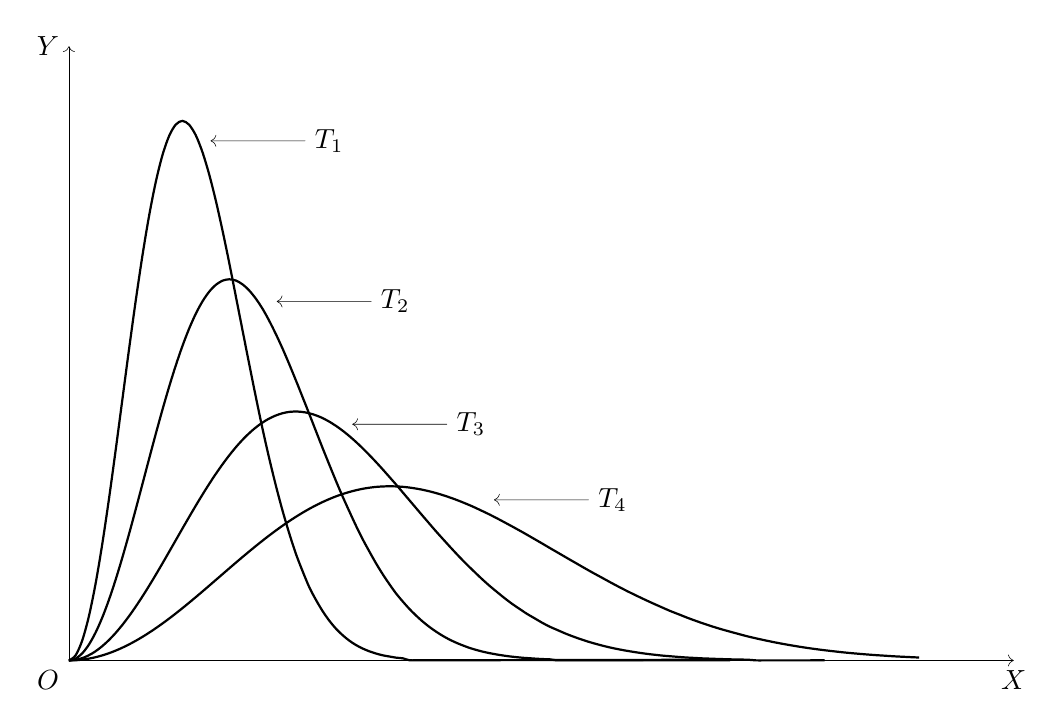
\begin{tikzpicture}[scale=1.2]
                \tkzDefPoint(0,0){O}
                \tkzDefPoint(10,0){X}
                \tkzDefPoint(0,6.5){Y}

                \tkzDrawSegment[->](O,X)
                \tkzDrawSegment[->](O,Y)

                \tkzLabelPoint[below](X){$X$}
                \tkzLabelPoint[left](Y){$Y$}
                \tkzLabelPoint[below left](O){$O$}

                \draw[smooth,thick,samples=100,domain=0:7] plot(\x,{5*4.80256*(10^-3)*4*3.1415*((6*\x)^2)*2.71828^(-(5.32*(6*\x)^2)/(2*1.3806*100))});
                \draw[smooth,thick,samples=100,domain=0:7] plot(\x,{5*1.69796*(10^-3)*4*3.1415*((6*\x)^2)*2.71828^(-(5.32*(6*\x)^2)/(2*1.3806*200))});
                \draw[smooth,thick,samples=100,domain=0:8] plot(\x,{5*6.00320*(10^-4)*4*3.1415*((6*\x)^2)*2.71828^(-(5.32*(6*\x)^2)/(2*1.3806*400))});
                \draw[smooth,thick,samples=100,domain=0:9] plot(\x,{5*2.12245*(10^-4)*4*3.1415*((6*\x)^2)*2.71828^(-(5.32*(6*\x)^2)/(2*1.3806*800))});

                \tkzDefPoint(1.5,5.5){T1L}
                \tkzDefPoint(2.2,3.8){T2L}
                \tkzDefPoint(3.0,2.5){T3L}
                \tkzDefPoint(4.5,1.7){T4L}

                \tkzDefShiftPoint[T1L](1,0){T1R}
                \tkzDefShiftPoint[T2L](1,0){T2R}
                \tkzDefShiftPoint[T3L](1,0){T3R}
                \tkzDefShiftPoint[T4L](1,0){T4R}

                \tkzDrawSegment[->](T1R,T1L)
                \tkzDrawSegment[->](T2R,T2L)
                \tkzDrawSegment[->](T3R,T3L)
                \tkzDrawSegment[->](T4R,T4L)

                \tkzLabelPoint[right](T1R){$T_1$}
                \tkzLabelPoint[right](T2R){$T_2$}
                \tkzLabelPoint[right](T3R){$T_3$}
                \tkzLabelPoint[right](T4R){$T_4$}
            \end{tikzpicture}
            \caption{温度和速率分布曲线的关系}
        \end{center}
    \end{figure}\\
    其中$T_1<T_2<T_3<T_4$。\\[3mm]
    温度较低,最概然速率较低,曲线最高点向左偏移,由于存在归一化条件,故曲线较为陡峭。\\[3mm]
    温度较高,最概然速率较高,曲线最高点向右偏移,由于存在归一化条件,故曲线较为平坦。

\newpage

\section{热力学基础}

\subsection{内能}
    热力学中将研究的物体称为热力学系统,与系统发生作用的环境称为外界。\\[3mm]
    热力学系统的能量依赖于系统的状态,这种能量称为内能。\\[3mm]
    气体的内能是分子动能和分子势能的总和。\\[3mm]
    气体为真实气体时的内能:
    \begin{large}
        \begin{equation*}
            E=F(V,T)
        \end{equation*}
    \end{large}\\
    气体为理想气体时的内能:
    \begin{large}
        \begin{equation*}
            E=F(T)
        \end{equation*}
    \end{large}\\
    由此可见,内能是系统状态的函数。\\[3mm]
    气体的分子动能和温度有关,气体的分子势能和体积有关。\\[3mm]
    气体为真实气体时,分子间相互作用不能忽略,分子势能不能忽略。\\[3mm]
    气体为理想气体时,分子间相互作用可以忽略,分子势能可以忽略。\\[3mm]
    理想气体的内能等于分子动能:
    \begin{large}
        \begin{equation*}
            E=\frac{i}{2}\cdot\frac{m}{M}\cdot R\cdot t
        \end{equation*}
    \end{large}\\
    因此计算理想气体的内能时,可以直接使用理想气体分子动能的公式。

\subsubsection{改变内能的方式}
    改变系统的内能有两个途径:\\[3mm]
    1.对热力学系统做功。\\[3mm]
    2.对热力学系统传递热量。\\[6mm]
    例如通过玻璃棒搅拌烧杯中的水,对其做功,可以使其温度升高,内能增加。\\[3mm]
    例如通过酒精灯加热烧杯中的水,传递热量,可以使其温度升高,内能增加。\\[3mm]
    由此可见,做功和传递热量,两者对于改变系统的内能是等效的。\\[3mm]

\newpage

    过去在习惯上,用焦作为功的单位,记作\si{J}。\\[3mm]
    过去在习惯上,用卡作为热的单位,记作\si{cal}。\\[3mm]
    焦耳通过热功当量实验测定了功和热的关系:
    \begin{large}
        \begin{equation*}
            1\si{cal}=4.186\si{J}
        \end{equation*}
    \end{large}\\
    现行的国际单位制中,功和热均用焦作为单位。\\[3mm]
    功是通过物体的宏观位移完成,是系统外物体的有规则位移与系统内分子的无规则运动的转换。\\[3mm]
    热是通过分子间相互作用完成,是系统外分子的无规则运动与系统内分子的无规则运动的转换。\\

\subsection{热力学第一定律}
    \textbf{热力学第一定律:}外界对系统传递的热量,等于系统的内能增量与对外做功的总和。\\[3mm]
    热力学第一定理的数学表达(宏观过程):
    \begin{large}
        \begin{equation*}
            Q=(E_2-E_1)+W
        \end{equation*}
    \end{large}\\
    热力学第一定律的数学表达(微观过程):
    \begin{large}
        \begin{equation*}
            \dif Q=\dif E+\dif W
        \end{equation*}
    \end{large}\\
    系统从外界吸热时,我们规定$\dif Q\;$为正值。\\[3mm]
    系统向外界放热时,我们规定$\dif Q\;$为负值。\\[3mm]
    系统对外界做功时,我们规定$\dif W$为正值。\\[3mm]
    系统受外界做功时,我们规定$\dif W$为负值。\\[3mm]
    系统的内能增加时,我们规定$\dif E\;$为正值。\\[3mm]
    系统的内能减小时,我们规定$\dif E\;$为负值。

\subsubsection{第一类永动机}
    第一类永动机指的是不消耗任何能量却可以不断对外做功的机器。\\[3mm]
    第一类永动机违背了热力学第一定律,因此不可能实现。

\newpage

\subsection{气体平衡过程中的功}
    \setcounter{equation}{0}
    气体平衡过程中的功的计算公式(宏观过程):
    \begin{large}
        \begin{equation*}
            W=\int_{V_1}^{V_2}P\cdot\dif V
        \end{equation*}
    \end{large}\\
    气体平衡过程中的功的计算公式(微观过程):
    \begin{large}
        \begin{equation*}
            \dif W=P\cdot\dif V
        \end{equation*}
    \end{large}\\
    假设有一气缸,面积为$S$,压强为$P$,压力为$F$,研究气缸在活塞由$l_1$移动至$l_2$时的做功情况。\\[3mm]
    气体平衡过程中的功的推导:
    \begin{align}
        W
        &=\int_{l_1}^{l_2}F\cdot\dif l\\[3mm]
        &=\int_{l_1}^{l_2}P\cdot S\cdot\dif l\\[3mm]
        &=\int_{V_1}^{V_2}P\cdot\dif W
    \end{align}\\
    气体在平衡过程中所做的功,是压强对体积的积分。\\[3mm]
    气体在平衡过程中所得到的功可以用$P-V$图表示:\vspace{5pt}
    \begin{figure}[h]
        \begin{center}
            \begin{tikzpicture}
                \tkzDefPoint(0,0){O}
                \tkzDefPoint(9,0){X}
                \tkzDefPoint(0,6){Y}

                \tkzDrawSegment[->](O,X)
                \tkzDrawSegment[->](O,Y)

                \tkzLabelPoint[above](X){$V$}
                \tkzLabelPoint[right](Y){$P$}

                \tkzDefPoint(1,5){A}
                \tkzDefPoint(5,1){B}
                \tkzDefPoint(1,0){A0}
                \tkzDefPoint(5,0){B0}

                \draw[smooth,thick,samples=100,domain=1:3,->] plot(\x,5/\x);
                \draw[smooth,thick,samples=100,domain=3:5] plot(\x,5/\x);

                \draw[smooth,thick,samples=100,domain=11.3088:40.9994] plot({5.099*cos(\x)},{5.099*sin(\x)});
                \draw[smooth,thick,samples=100,domain=40.9994:78.6900,<-] plot({5.099*cos(\x)},{5.099*sin(\x)});

                \tkzDrawSegment[dashed](A,A0)
                \tkzDrawSegment[dashed](B,B0)

                \tkzDrawPoint[fill=white](A)
                \tkzDrawPoint[fill=white](B)

                \tkzLabelPoint[above right](A){$A_1(P_1,V_1,T_1)$}
                \tkzLabelPoint[right](B){$A_2(P_2,V_2,T_2)$}
            \end{tikzpicture}
            \caption{气体在平衡过程中所做的功}
        \end{center}
    \end{figure}\\
    其中曲线下方的面积表示功,由图可知做功的多少与过程有关。\\[3mm]
    由于内能与过程无关(内能是过程的函数),而做功与过程有关,故吸收热量与过程有关。

\newpage

\subsection{气体的等体过程}
    \setcounter{equation}{0}
    气体的等体过程的特征是体积不变,即$V_1=V_2=V$。\\[3mm]
    气体的等体过程在$P-V$图上表现为平行于$P$轴的直线,称为等体线:\vspace{5pt}
    \begin{figure}[h]
        \begin{center}
            \begin{tikzpicture}[scale=1.0]
                \tkzDefPoint(0,0){O}
                \tkzDefPoint(8,0){X}
                \tkzDefPoint(0,6){Y}

                \tkzDrawSegment[->](O,X)
                \tkzDrawSegment[->](O,Y)

                \tkzLabelPoint[above](X){$V$}
                \tkzLabelPoint[right](Y){$P$}

                \tkzDefPoint(6,2){A1}
                \tkzDefPoint(6,4){A2}

                \tkzDefPoint(0,2){P1}
                \tkzDefPoint(0,4){P2}

                \tkzDefPoint(6,0){V}

                \tkzDrawSegment[dashed](P1,A1);
                \tkzDrawSegment[dashed](P2,A2);
                \tkzDrawSegment[dashed](V,A1);

                \tkzDrawSegment[thick,->](A1,A2);

                \tkzLabelPoint[right](A1){$A_1(P_1,V,T_1)$}
                \tkzLabelPoint[right](A2){$A_2(P_2,V,T_2)$}

                \tkzLabelPoint[left](P1){$P_1$}
                \tkzLabelPoint[left](P2){$P_2$}

                \tkzLabelPoint[below](V){$V$}

                \tkzDrawPoint[fill=white](A1)
                \tkzDrawPoint[fill=white](A2)
            \end{tikzpicture}
            \caption{气体的等体过程}
        \end{center}
    \end{figure}\\
    气体的等体过程中的热量变化:
    \begin{large}
        \begin{equation*}
            Q_V=\frac{i}{2}\cdot\frac{m}{M}\cdot R\cdot(T_2-T_1)
        \end{equation*}
    \end{large}\\
    气体的等体过程中的内能变化:
    \begin{large}
        \begin{equation*}
            \Delta E=\frac{i}{2}\cdot\frac{m}{M}\cdot R\cdot(T_2-T_1)
        \end{equation*}
    \end{large}\\
    气体的等体过程中的做功情况:
    \begin{large}
        \begin{equation*}
            W=0\vphantom{\frac{a}{b}}
        \end{equation*}
    \end{large}\\
    在等体升温的过程中,理想气体吸收的热量,全部转化为其内能的增加,不向外界做功。\\[3mm]
    在等体降温的过程中,理想气体放出的热量,全部来自于其内能的减少,不受外界做功。\\[3mm]
    由于压强和温度成正比,故向上的等体线压强增大温度升高,是等体升温过程。\\[3mm]
    由于压强和温度成正比,故向下的等体线压强减小温度下降,是等体降温过程。

\newpage

    由于等体过程的体积为定值:
    \begin{align}
        &W=\int_{V_1}^{V_2} P\cdot\dif V~~~~\\[4mm]
        &W=0
    \end{align}\\
    根据理想气体的内能的公式:
    \begin{align}
        &~~~~~~~~~~\Delta E=E_2-E_1\\[4mm]
        &~~~~~~~~~~\Delta E=\frac{i}{2}\cdot\frac{m}{M}\cdot R\cdot T_2-\frac{i}{2}\cdot\frac{m}{M}\cdot R\cdot T_1\\[4mm]
        &~~~~~~~~~~\Delta E=\frac{i}{2}\cdot\frac{m}{M}\cdot R\cdot (T_2-T_1)
    \end{align}\\
    由热力学第一定律可以得到:
    \begin{align}
        &Q_V=(E_2-E_1)+W\\[4mm]
        &Q_V=\Delta E+W\\[4mm]
        &Q_V=\frac{i}{2}\cdot\frac{m}{M}\cdot R\cdot (T_2-T_1)~~~~~~
    \end{align}\\
    由此证明了气体的等体过程的相关规律。

\newpage

\subsection{气体的等压过程}
    \setcounter{equation}{0}
    气体的等压过程的特征是压强不变,即$P_1=P_2=P$。\\[3mm]
    气体的等压过程在$P-V$图上表现为平行于$V$轴的直线,称为等压线:\vspace{5pt}
    \begin{figure}[h]
        \begin{center}
            \begin{tikzpicture}[scale=1.0]
                \tkzDefPoint(0,0){O}
                \tkzDefPoint(8,0){X}
                \tkzDefPoint(0,6){Y}

                \tkzDrawSegment[->](O,X)
                \tkzDrawSegment[->](O,Y)

                \tkzLabelPoint[above](X){$V$}
                \tkzLabelPoint[right](Y){$P$}

                \tkzDefPoint(3,4){A1}
                \tkzDefPoint(6,4){A2}

                \tkzDefPoint(3,0){V1}
                \tkzDefPoint(6,0){V2}

                \tkzDefPoint(0,4){P}

                \tkzDrawSegment[dashed](V1,A1);
                \tkzDrawSegment[dashed](V2,A2);
                \tkzDrawSegment[dashed](P,A1);

                \tkzDrawSegment[thick,->](A1,A2);

                \tkzLabelPoint[above](A1){$A_1(P,V_1,T_1)$}
                \tkzLabelPoint[above](A2){$A_2(P,V_2,T_2)$}

                \tkzLabelPoint[left](P){$P$}

                \tkzLabelPoint[below](V1){$V_1$}
                \tkzLabelPoint[below](V2){$V_2$}

                \tkzDrawPoint[fill=white](A1)
                \tkzDrawPoint[fill=white](A2)
            \end{tikzpicture}
            \caption{气体的等压过程}
        \end{center}
    \end{figure}\\
    气体的等压过程中的热量变化:
    \begin{large}
        \begin{align*}
            &Q_P=\frac{i+2}{2}\cdot\frac{m}{M}\cdot R\cdot(T_2-T_1)
        \end{align*}
    \end{large}\\
    气体的等压过程中的内能变化:
    \begin{large}
        \begin{align*}
            &\Delta E=\frac{i}{2}\cdot\frac{m}{M}\cdot R\cdot(T_2-T_1)
        \end{align*}
    \end{large}\\
    气体的等压过程中的做功情况:
    \begin{large}
        \begin{align*}
            &W=\frac{m}{M}\cdot R\cdot(T_2-T_1)
        \end{align*}
    \end{large}\\
    在等压升温的过程中,理想气体吸收的热量,部分转化为其内能的增加,部分用于向外界做功。\\[3mm]
    在等压降温的过程中,理想气体放出的热量,部分来自于其内能的减少,部分源于受外界做功。\\[3mm]
    由于体积和温度成正比,故向右的等体线体积增大温度升高,是等压升温过程。\\[3mm]
    由于体积和温度成正比,故向左的等体线体积减小温度下降,是等压降温过程。

\newpage

    由于等压过程的压强为定值:
    \begin{align}
        &W=\int_{V_1}^{V_2} P\cdot\dif V~~~~~~~~\\[4mm]
        &W=P\cdot(V_2-V_1)
    \end{align}\\
    根据克拉伯龙方程可以得到:
    \begin{align}
        &~~W=P\cdot\left(\frac{m}{M\cdot P}\cdot R\cdot T_2-\frac{m}{M\cdot P}\cdot R\cdot T_1\right)\\[4mm]
        &~~W=\frac{m}{M}\cdot R\cdot T_2-\frac{m}{M}\cdot R\cdot T_1\\[4mm]
        &~~W=\frac{m}{M}\cdot R\cdot (T_2-T_1)
    \end{align}\\
    根据理想气体的内能的公式:
    \begin{align}
        &\Delta E=E_2-E_1\\[4mm]
        &\Delta E=\frac{i}{2}\cdot\frac{m}{M}\cdot R\cdot T_2-\frac{i}{2}\cdot\frac{m}{M}\cdot R\cdot T_1~~~~~~~~\\[4mm]
        &\Delta E=\frac{i}{2}\cdot\frac{m}{M}\cdot R\cdot (T_2-T_1)
    \end{align}\\
    由热力学第一定律可以得到:
    \begin{align}
        &~~~~~~~~Q_P=(E_2-E_1)+W\\[4mm]
        &~~~~~~~~Q_P=\Delta E+W\\[4mm]
        &~~~~~~~~Q_P=\frac{i}{2}\cdot\frac{m}{M}\cdot R\cdot(T_2-T_1)+\frac{m}{M}\cdot R\cdot(T_2-T_1)\\[4mm]
        &~~~~~~~~Q_P=\frac{i+2}{2}\cdot\frac{m}{M}\cdot R\cdot(T_2-T_1)
    \end{align}\\
    由此证明了气体的等压过程的相关规律。

\newpage

\subsection{气体的热容量}
    热容量衡量了一定量的物质上升单位温度所需吸收的热量。\\[3mm]
    热容量是一个标量,通常用符号$C$表示,单位是\si{J/K}。\\[3mm]
    热容量的定义式:
    \begin{large}
        \begin{equation*}
            Q=\int_{T_1}^{T_2}C\cdot\dif T
        \end{equation*}
    \end{large}\\
    比热容量衡量了一定质量的物质上升单位温度所需吸收的热量。\\[3mm]
    比热容量是一个标量,通常用符号$c$表示,单位是\si{J/(K\cdot kg)}。\\[3mm]
    比热容量的定义式:
    \begin{large}
        \begin{equation*}
            Q=m\cdot\int_{T_1}^{T_2}c\cdot\dif T
        \end{equation*}
    \end{large}\\
    摩尔热容量衡量了单位物质的量的物质上升单位温度所吸收的热量。\\[3mm]
    摩尔热容量是一个标量,通常用符号$C_m$表示,单位是\si{J/(K\cdot mol)}。\\[3mm]
    摩尔热容量的定义式:
    \begin{large}
        \begin{equation*}
            Q=\frac{m}{M}\cdot\int_{T_1}^{T_2}C_m\cdot\dif T\\[3mm]
        \end{equation*}
    \end{large}\\
    对摩尔热容量的定义式两侧取微分:
    \setcounter{equation}{0}
    \begin{align}
        &Q=\frac{m}{M}\cdot\int C_m\cdot\dif T\\[4mm]
        &\dif Q=\frac{m}{M}\cdot C_m\cdot\dif T\\[4mm]
        &\dif Q\cdot\frac{M}{m}=C_m\cdot\dif T\\[4mm]
        &C_m=\frac{M}{m}\cdot\frac{\dif Q}{\dif T}
    \end{align}\\
    摩尔热容量的计算公式:
    \begin{large}
        \begin{equation*}
            C_m=\frac{M}{m}\cdot\frac{\dif Q}{\dif T}    
        \end{equation*}
    \end{large}\\
    摩尔热容量正比于热容对温度的导数。

\newpage

\subsubsection{等体摩尔热容量}
    等体摩尔热容量指的是气体在等体过程中的摩尔热容量,通常用符号$C_{V_m}$表示。\\[3mm]
    等体摩尔热容量的计算公式:
    \begin{large}
        \begin{equation*}
            C_{V_m}=\frac{i}{2}\cdot R
        \end{equation*}
    \end{large}\\
    等体摩尔热容量的推导过程:
    \setcounter{equation}{0}
    \begin{align}
        C_{V_m}
        &=\frac{M}{m}\cdot\frac{\dif Q_V}{\dif T}\\[4mm]
        &=\frac{M}{m}\cdot\frac{\dif}{\dif T}\cdot\left(\frac{i}{2}\cdot\frac{m}{M}\cdot R\cdot T\right)\\[4mm]
        &=\frac{i}{2}\cdot\frac{M}{m}\cdot\frac{m}{M}\cdot R\cdot\frac{\dif T}{\dif T}\\[4mm]
        &=\frac{i}{2}\cdot R\cdot\frac{\dif T}{\dif T}\\[4mm]
        &=\frac{i}{2}\cdot R
    \end{align}\\
    等体摩尔热容量只和气体自由度有关,等体摩尔热容量是一个无关温度的定值。\\[3mm]
    等体过程的热量还可以表示为:
    \begin{large}
        \begin{equation*}
            Q_V=\frac{m}{M}\cdot C_{V_m}\cdot(T_2-T_1)
        \end{equation*}
    \end{large}\\
    理想气体的等体摩尔容量分别为:\vspace{5pt}
    \begin{table}[h]
        \begin{center}
            \begin{tabular}{p{80pt}|p{60pt}|p{130pt}}
                \hline
                气体类型&自由度&等体摩尔容量\\ \hline
                单原子气体&$i=3$&$C_{V_m}=12.5$~\si{J/(K\cdot mol)}\\ \hline
                双原子气体&$i=5$&$C_{V_m}=20.8$~\si{J/(K\cdot mol)}\\ \hline
                多原子气体&$i=6$&$C_{V_m}=24.9$~\si{J/(K\cdot mol)}\\ \hline
            \end{tabular}
            \caption{理想气体的等体摩尔容量}
        \end{center}
    \end{table}\\
    实际气体的等体摩尔容量,单原子和双原子气体与理论值相近,多原子气体与理论值相差较大。

\newpage

\subsubsection{等压摩尔热容量}
    等压摩尔热容量指的是气体在等压过程中的摩尔热容量,通常用符号$C_{P_m}$表示。\\[3mm]
    等压摩尔热容量的计算公式:
    \begin{large}
        \begin{equation*}
            C_{P_m}=\frac{i+2}{2}\cdot R
        \end{equation*}
    \end{large}\\
    等压摩尔热容量的推导过程:
    \setcounter{equation}{0}
    \begin{align}
        C_{P_m}
        &=\frac{M}{m}\cdot\frac{\dif Q_V}{\dif T}\\[4mm]
        &=\frac{M}{m}\cdot\frac{\dif}{\dif T}\cdot\left(\frac{i+2}{2}\cdot\frac{m}{M}\cdot R\cdot T\right)\\[4mm]
        &=\frac{i+2}{2}\cdot\frac{M}{m}\cdot\frac{m}{M}\cdot R\cdot\frac{\dif T}{\dif T}\\[4mm]
        &=\frac{i+2}{2}\cdot R\cdot\frac{\dif T}{\dif T}\\[4mm]
        &=\frac{i+2}{2}\cdot R
    \end{align}\\
    等压摩尔热容量只和气体自由度有关,等压摩尔热容量是一个无关温度的定值。\\[3mm]
    等压过程的热量还可以表示为:
    \begin{large}
        \begin{equation*}
            Q_P=\frac{m}{M}\cdot C_{P_m}\cdot(T_2-T_1)
        \end{equation*}
    \end{large}\\
    理想气体的等压摩尔容量分别为:\vspace{5pt}
    \begin{table}[h]
        \begin{center}
            \begin{tabular}{p{80pt}|p{60pt}|p{130pt}}
                \hline
                气体类型&自由度&等体摩尔容量\\ \hline
                单原子气体&$i=3$&$C_{P_m}=20.8$~\si{J/(K\cdot mol)}\\ \hline
                双原子气体&$i=5$&$C_{P_m}=29.1$~\si{J/(K\cdot mol)}\\ \hline
                多原子气体&$i=6$&$C_{P_m}=33.2$~\si{J/(K\cdot mol)}\\ \hline
            \end{tabular}
            \caption{理想气体的等压摩尔容量}
        \end{center}
    \end{table}\\
    实际气体的等压摩尔容量,单原子和双原子气体与理论值相近,多原子气体与理论值相差较大。

\newpage

\subsubsection{热容比}
    热容比定义为等压摩尔热容与等体摩尔热容的比值,通常用符号$\gamma$表示。\\[3mm]
    热容比定义的数学表达:
    \begin{large}
        \begin{equation*}
            \gamma=\frac{C_{P_m}}{C_{V_m}}=\frac{i+2}{i}
        \end{equation*}
    \end{large}\\
    理想气体的热容比分别为:\vspace{5pt}
    \begin{table}[h]
        \begin{center}
            \begin{tabular}{p{80pt}|p{60pt}|p{80pt}}
                \hline
                气体类型&自由度&热容比\\ \hline
                单原子气体&$i=3$&$\gamma=1.67$\\ \hline
                双原子气体&$i=5$&$\gamma=1.40$\\ \hline
                多原子气体&$i=6$&$\gamma=1.33$\\ \hline
            \end{tabular}
            \caption{理想气体的热容比}
        \end{center}
    \end{table}

\subsubsection{迈耶公式}
    迈耶公式指出了等压摩尔热容量和等体摩尔热容量的差恒普适气体常量常量$R$。\\[3mm]
    迈耶公式的数学表达:
    \begin{large}
        \begin{equation*}
            C_{P_m}-C_{V_m}=R
        \end{equation*}
    \end{large}\\
    迈耶公式的推导过程:
    \setcounter{equation}{0}
    \begin{align}
        &C_{P_m}-C_{V_m}=\frac{i+2}{2}\cdot R-\frac{i}{2}\cdot R\\[3mm]
        &C_{P_m}-C_{V_m}=R
    \end{align}\\
    对于实际气体的摩尔热容,单原子和双原子气体与理论值相近,多原子气体与理论值有所偏离,
    然而无论哪种气体,均基本遵循迈耶公式,即两种摩尔热容的差为普适气体常量。\\[3mm]
    由此可见,迈耶公式有超越等体摩尔热容和等压摩尔热容的普适意义。\\[3mm]
    除此之外,迈耶公式说明了升高相同温度,等压过程相比等体过程需要吸收更多能量。

\newpage

\subsection{气体的等温过程}
    \setcounter{equation}{0}
    气体的等温过程的特征是温度不变,即$T_1=T_2=T$。\\[3mm]
    气体的等温过程在$P-V$图上表现为等轴双曲线,称为等温线:\vspace{5pt}
    \begin{figure}[h]
        \begin{center}
            \begin{tikzpicture}[scale=1.0]
                \tkzDefPoint(0,0){O}
                \tkzDefPoint(8,0){X}
                \tkzDefPoint(0,6){Y}

                \tkzDrawSegment[->](O,X)
                \tkzDrawSegment[->](O,Y)

                \tkzLabelPoint[above](X){$V$}
                \tkzLabelPoint[right](Y){$P$}

                \tkzDefPoint(1,5){A1}
                \tkzDefPoint(5,1){A2}

                \tkzDefPoint(1,0){V1}
                \tkzDefPoint(5,0){V2}

                \tkzDefPoint(0,5){P1}
                \tkzDefPoint(0,1){P2}

                \tkzDrawSegment[dashed](V1,A1);
                \tkzDrawSegment[dashed](V2,A2);
                \tkzDrawSegment[dashed](P1,A1);
                \tkzDrawSegment[dashed](P2,A2);

                \draw[smooth,thick,samples=100,domain=1:5,->] plot(\x,5/\x);

                \tkzLabelPoint[right](A1){$A_1(P_1,V_1,T)$}
                \tkzLabelPoint[right](A2){$A_2(P_2,V_2,T)$}

                \tkzLabelPoint[left](P1){$P_1$}
                \tkzLabelPoint[left](P2){$P_2$}

                \tkzLabelPoint[below](V1){$V_1$}
                \tkzLabelPoint[below](V2){$V_2$}

                \tkzDrawPoint[fill=white](A1)
                \tkzDrawPoint[fill=white](A2)
            \end{tikzpicture}
            \caption{气体的等温过程}
        \end{center}
    \end{figure}\\
    气体的等温过程中的热量变化:
    \begin{large}
        \begin{align*}
            &Q_T=\frac{m}{M}\cdot R\cdot T\cdot\ln{\frac{V_2}{V_1}}\\[2mm]
            &Q_T=\frac{m}{M}\cdot R\cdot T\cdot\ln{\frac{P_1}{P_2}}
        \end{align*}
    \end{large}\\
    气体的等温过程中的做功情况:
    \begin{large}
        \begin{align*}
            &W=\frac{m}{M}\cdot R\cdot T\cdot\ln{\frac{V_2}{V_1}}\\[2mm]
            &W=\frac{m}{M}\cdot R\cdot T\cdot\ln{\frac{P_1}{P_2}}
        \end{align*}
    \end{large}\\
    气体的等温过程中的内能变化:
    \begin{large}
        \begin{equation*}
            \Delta E=0
        \end{equation*}
    \end{large}\\
    在等温膨胀中,理想气体向外界所作的功,全部来自于其吸收的热量,内能不变。\\[3mm]
    在等温压缩中,理想气体受外界所作的功,全部转化为其放出的热量,内能不变。

\newpage

    由于等压过程的温度为定值:
    \begin{align}
        &\Delta E=E_2-E_1\\[4mm]
        &\Delta E=0
    \end{align}\\
    根据克拉伯龙方程可以得到:
    \begin{align}
        &~~~~W=\int_{V_1}^{V_2} P\cdot\dif V\\[4mm]
        &~~~~W=\int_{V_1}^{V_2} \frac{m}{M\cdot V}\cdot R\cdot T\cdot\dif V\\[4mm]
        &~~~~W=\frac{m}{M}\cdot R\cdot T\cdot\int_{V_1}^{V_2} \frac{1}{V}\cdot\dif V\\[4mm]
        &~~~~W=\frac{m}{M}\cdot R\cdot T\cdot\left(\ln{V_2}-\ln{V_1}\right)\\[4mm]
        &~~~~W=\frac{m}{M}\cdot R\cdot T\cdot\ln{\frac{V_2}{V_1}}
    \end{align}\\
    由热力学第一定律可以得到:
    \begin{align}
        &Q_T=(E_2-E_1)+W\\[4mm]
        &Q_T=\Delta E+W\\[4mm]
        &Q_T=\frac{m}{M}\cdot R\cdot T\cdot\ln{\frac{V_2}{V_1}}\\[4mm]
        &Q_T=\frac{m}{M}\cdot R\cdot T\cdot\ln{\frac{P_1}{P_2}}~~~~~~~~~~
    \end{align}\\
    其中最后一步运用了玻意耳定律:
    \begin{align}
        P_1\cdot V_1=P_2\cdot V_2~~\Rightarrow~~\frac{P_1}{P_2}=\frac{V_2}{V_1}
    \end{align}\\
    由此证明了气体的等温过程的相关规律。

\newpage

\subsection{气体的绝热过程}
    \setcounter{equation}{0}
    气体的绝热过程的特指是对外绝热,即$Q=0$。\\[3mm]
    气体的绝热过程在$P-V$图上表现为一根曲线,称为绝热线:
    \begin{figure}[h]
        \begin{center}
            \begin{tikzpicture}[scale=1.0]
                \tkzDefPoint(0,0){O}
                \tkzDefPoint(8,0){X}
                \tkzDefPoint(0,6){Y}

                \tkzDrawSegment[->](O,X)
                \tkzDrawSegment[->](O,Y)

                \tkzLabelPoint[above](X){$V$}
                \tkzLabelPoint[right](Y){$P$}

                \tkzDefPoint(1,5){A1}
                \tkzDefPoint(5,0.53){A2}

                \tkzDefPoint(1,0){V1}
                \tkzDefPoint(5,0){V2}

                \tkzDefPoint(0,5){P1}
                \tkzDefPoint(0,0.53){P2}

                \tkzDrawSegment[dashed](V1,A1);
                \tkzDrawSegment[dashed](V2,A2);
                \tkzDrawSegment[dashed](P1,A1);
                \tkzDrawSegment[dashed](P2,A2);

                \draw[smooth,thick,samples=100,domain=1:5,->] plot(\x,5/\x^1.4);

                \tkzLabelPoint[right](A1){$A_1(P_1,V_1,T_1)$}
                \tkzLabelPoint[right](A2){$A_2(P_2,V_2,T_2)$}

                \tkzLabelPoint[left](P1){$P_1$}
                \tkzLabelPoint[left](P2){$P_2$}

                \tkzLabelPoint[below](V1){$V_1$}
                \tkzLabelPoint[below](V2){$V_2$}

                \tkzDrawPoint[fill=white](A1)
                \tkzDrawPoint[fill=white](A2)
            \end{tikzpicture}
            \caption{气体的绝热过程}
        \end{center}
    \end{figure}\\
    气体的绝热过程中的内能变化:
    \begin{large}
        \begin{align*}
            &\Delta E=\frac{i}{2}\cdot\frac{m}{M}\cdot R\cdot(T_2-T_1)\\[3mm]
            &\Delta E=\frac{m}{M}\cdot C_{V_m}\cdot(T_2-T_1)
        \end{align*}
    \end{large}\\
    气体的绝热过程中的做功情况:
    \begin{large}
        \begin{align*}
            &W=-\frac{i}{2}\cdot\frac{m}{M}\cdot R\cdot(T_2-T_1)\\[3mm]
            &W=-\frac{m}{M}\cdot C_{V_m}\cdot(T_2-T_1)
        \end{align*}
    \end{large}\\
    气体的绝热过程中的热量变化:
    \begin{large}
        \begin{equation*}
            Q=0
        \end{equation*}
    \end{large}\\
    在绝热膨胀中,理想气体向外界所作的功,全部来自于其内能的减少,不吸收热量。\\[3mm]
    在绝热压缩中,理想气体受外界所作的功,全部转化为其内能的增加,不放出热量。\\[3mm]

\newpage

    根据理想气体的内能的公式:
    \begin{align}
        &\Delta E=E_2-E_1\\[3mm]
        &\Delta E=\frac{i}{2}\cdot\frac{m}{M}\cdot R\cdot (T_2-T_1)\\[3mm]
        &\Delta E=\frac{m}{M}\cdot C_{V_m}\cdot(T_2-T_1)
    \end{align}\\
    由热力学第一定律可以得到:
    \begin{align}
        &Q=(E_2-E_1)+W\\[3mm]
        &0=\Delta E+W\\[3mm]
        &W=-\Delta E\\[3mm]
        &W=-\frac{i}{2}\cdot\frac{m}{M}\cdot R\cdot (T_2-T_1)~~\\[3mm]
        &W=-\frac{m}{M}\cdot C_{V_m}\cdot(T_2-T_1)
    \end{align}\\
    由此证明了绝热过程的相关规律。

\subsubsection{绝热过程中气体状态参量间的关系}
    \setcounter{equation}{0}
    绝热过程中,气体的压强体积温度均在变化,但是三者间实际上仍然存在一组额外关系。\\[3mm]
    绝热过程中的对外绝热:
    \begin{align}
        &\dif E+\dif W=0\\[3mm]
        &P\cdot \dif V=-\dif E\\[3mm]
        &P\cdot \dif V=-\frac{m}{M}\cdot C_{V_m}\cdot\dif T
    \end{align}\\
    对克拉伯龙方程取微分:
    \begin{align}
        &P\cdot V=\frac{m}{M}\cdot R\cdot T\\[3mm]
        &P\cdot\dif V+V\cdot\dif P=\frac{m}{M}\cdot R\cdot \dif T
    \end{align}\\
    由此得到了两组绝热过程中关于$\dif P$、$\dif V$、$\dif T$的关系式。

\newpage

    由此得到了一个方程组:
    \begin{align}
        \begin{cases}
            ~P\cdot\dif V=-\dfrac{m}{M}\cdot C_{V_m}\cdot\dif T\\[2mm]
            ~P\cdot\dif V+V\cdot\dif P=\dfrac{m}{M}\cdot R\cdot \dif T\\[2mm]
        \end{cases}
    \end{align}\\
    由第一个方程反解$\dif T$:
    \begin{align}
        &\dif T\cdot C_{V_m}=-\frac{m}{M}\cdot P\cdot\dif V~~~~\\[3mm]
        &\dif T=-\frac{M}{m}\cdot\frac{1}{C_{V_m}}\cdot P\cdot\dif V
    \end{align}\\
    在第二个方程代入$\dif T$:
    \begin{align}
        &~~~~P\cdot\dif V+V\cdot\dif P=\dfrac{m}{M}\cdot R\cdot \dif T\\[3mm]
        &~~~~P\cdot\dif V+V\cdot\dif P=-\frac{m}{M}\cdot R\cdot\left(\frac{M}{m}\cdot\frac{1}{C_{V_m}}\cdot P\cdot\dif V\right)\\[3mm]
        &~~~~P\cdot\dif V+V\cdot\dif P=-\frac{1}{C_{V_m}}\cdot P\cdot\dif V
    \end{align}\\
    对其变形代入迈耶公式:
    \begin{align}
        &~~C_{V_m}\cdot(P\cdot\dif V+V\cdot\dif P)=-R\cdot P\cdot\dif V\\[3mm]
        &~~C_{V_m}\cdot(P\cdot\dif V+V\cdot\dif P)=-(C_{P_m}-C_{V_m})\cdot R\cdot P\cdot\dif V\\[3mm]
        &~~C_{V_m}\cdot(P\cdot\dif V+V\cdot\dif P)=(C_{V_m}-C_{P_m})\cdot R\cdot P\cdot\dif V\\[3mm]
        &~~C_{V_m}\cdot P\cdot\dif V+C_{V_m}\cdot V\cdot\dif P=C_{V_m}\cdot P\cdot\dif V-C_{P_m}\cdot P\cdot\dif V\\[3mm]
        &~~C_{V_m}\cdot V\cdot\dif P+C_{P_m}\cdot P\cdot\dif V=0
    \end{align}\\
    将两侧同除$P\cdot V$:
    \begin{align}
        &\frac{\dif P}{P}\cdot C_{V_m}+\frac{\dif V}{V}\cdot C_{P_m}=0
    \end{align}\\
    将两侧同除$C_{V_m}$:
    \begin{align}
        &\frac{\dif P}{P}\cdot\frac{C_{V_m}}{C_{V_m}}+\frac{\dif V}{V}\cdot\frac{C_{P_m}}{C_{V_m}}=0\\[3mm]
        &\frac{\dif P}{P}+\frac{\dif V}{V}\cdot\gamma=0
    \end{align}\\
    由此我们将$P,\dif P$与$V,\dif V$分离。

\newpage

    对以上得到的结论积分可得:
    \begin{align}
        &\int\frac{1}{P}\cdot\dif P+\gamma\cdot\int\frac{1}{V}\cdot\dif V=C\\[3mm]
        &\ln{P}+\gamma\cdot\ln{V}=C\\[3mm]
        &e^{\ln{P}+\gamma\cdot\ln{V}}=C\\[3mm]
        &e^{\ln{P}}+e^{\gamma\cdot\ln{V}}=C\\[3mm]
        &P\cdot V^{\gamma}=C
    \end{align}\\
    绝热过程压强和体积的关系(第一种表达):
    \begin{large}
        \begin{equation*}
            P_1\cdot V_1^{\gamma}=P_2\cdot V_2^{\gamma}
        \end{equation*}
    \end{large}\\
    绝热过程压强和体积的关系(第二种表达):
    \begin{large}
        \begin{equation*}
            P\cdot V^{\gamma}=C
        \end{equation*}
    \end{large}\\
    由克拉伯龙方程代换压强:
    \begin{align}
        &P\cdot V^{\gamma}=C\\[3mm]
        &V^{\gamma}\cdot\left(\frac{m}{M}\cdot\frac{1}{V}\cdot R\cdot T\right)=C\\[3mm]
        &V^{\gamma-1}\cdot T\cdot\left(\frac{m}{M}\cdot R\right)=C\\[3mm]
        &V^{\gamma-1}\cdot T=C
    \end{align}\\
    由克拉伯龙方程代换体积:
    \begin{align}
        &P\cdot V^{\gamma}=C\\[3mm]
        &P\cdot\left(\frac{m}{M}\cdot\frac{1}{P}\cdot R\cdot T\right)^{\gamma}=C\\[3mm]
        &P^{1-\gamma}\cdot T^{\gamma}\cdot\left(\frac{m}{M}\cdot R\right)^{\gamma}=C\\[3mm]
        &P^{1-\gamma}\cdot T^{\gamma}=C
    \end{align}\\
    由此得到了另外两组关系。

\newpage

    绝热过程体积和温度的关系(第一种表达):
    \begin{large}
        \begin{equation*}
            V_1^{\gamma-1}\cdot T_1=V_2^{\gamma-1}\cdot T_2
        \end{equation*}
    \end{large}\\
    绝热过程体积和温度的关系(第二种表达):
    \begin{large}
        \begin{equation*}
            V^{\gamma-1}\cdot T=C
        \end{equation*}
    \end{large}\\
    绝热过程压强和温度的关系(第一种表达):
    \begin{large}
        \begin{equation*}
            P_1^{1-\gamma}\cdot T_1^{\gamma}=P_2^{1-\gamma}\cdot T_2^{\gamma}
        \end{equation*}
    \end{large}\\
    绝热过程压强和温度的关系(第二种表达):
    \begin{large}
        \begin{equation*}
            P^{1-\gamma}\cdot T^{\gamma}=C
        \end{equation*}
    \end{large}\\
    由此证明了绝热过程中各个状态参量间存在的一组额外关系。\\[3mm]
    因此绝热过程中只要知道一个参量的数值,就一定可以求出另外两个参量。

\subsubsection{绝热过程和等温过程的关系}
    \setcounter{equation}{0}
    根据之前的推导,绝热过程满足的方程为$P\cdot V^{\gamma}=C$。\\[3mm]
    根据之前的推导,等温过程满足的方程为$P\cdot V=C$。\\[3mm]
    因此绝热线和等温线实际上非常相似:
    \begin{figure}[h]
        \begin{center}
            \begin{tikzpicture}[scale=0.8]
                \tkzDefPoint(0,0){O}
                \tkzDefPoint(8,0){X}
                \tkzDefPoint(0,6.3){Y}

                \tkzDrawSegment[->](O,X)
                \tkzDrawSegment[->](O,Y)

                \tkzLabelPoint[above](X){$V$}
                \tkzLabelPoint[right](Y){$P$}

                \draw[smooth,thick,samples=100,domain=1.12:5.8] plot(\x,6.9644/\x^1.8);
                \draw[smooth,dashed,thick,samples=100,domain=0.8:5.3] plot(\x,4.0000/\x);

                \tkzDefPoint(2,2){A}
                \tkzDrawPoint[fill=white](A)
                \tkzLabelPoint[right](A){$A$}

                \tkzDefPoint(5,5){Q1}
                \tkzDefPoint(6,5){Q2}
                \tkzDefPoint(5,4){T1}
                \tkzDefPoint(6,4){T2}

                \tkzDrawSegment(Q1,Q2)
                \tkzDrawSegment[dashed](T1,T2)

                \tkzLabelPoint[right](Q2){绝热线}
                \tkzLabelPoint[right](T2){等温线}
            \end{tikzpicture}
            \caption{绝热过程和等温过程}
        \end{center}
    \end{figure}\\[3mm]
    由图可见,绝热线的切线斜率的绝对值总是大于等温线,绝热线比等温线更陡峭。

\newpage

    由于等温过程的方程为:
    \begin{align}
        &P\cdot V=C~~\rightarrow~~P=\frac{C}{V}
    \end{align}\\
    故等温过程中的导数为:
    \begin{align}
        \frac{\dif P}{\dif V}&=\frac{\dif}{\dif V}\cdot\frac{C}{V}\\[3mm]
        \frac{\dif P}{\dif V}&=-\frac{C}{V^2}\\[3mm]
        \frac{\dif P}{\dif V}&=-\frac{P\cdot V}{V^2}\\[3mm]
        \frac{\dif P}{\dif V}&=-\frac{P}{V}
    \end{align}\\
    由于绝热过程的方程为:
    \begin{align}
        &P\cdot V^{\gamma}=C~~\rightarrow~~P=\frac{C}{V^{\gamma}}
    \end{align}\\
    故绝热过程中的导数为:
    \begin{align}
        \frac{\dif P}{\dif V}&=\frac{\dif}{\dif V}\cdot\frac{C}{V^{\gamma}}\\[3mm]
        \frac{\dif P}{\dif V}&=-\gamma\cdot\frac{C}{V^{^{\gamma}+1}}\\[3mm]
        \frac{\dif P}{\dif V}&=-\gamma\cdot\frac{P\cdot V}{V^{\gamma+1}}\\[3mm]
        \frac{\dif P}{\dif V}&=-\gamma\cdot\frac{P}{V}
    \end{align}\\
    根据热容比的定义可知其满足$\gamma>1$:\vspace{3pt}
    \begin{large}
        \begin{equation*}
            \left|-\gamma\cdot\frac{P}{V}\right|>\left|-\frac{P}{V}\right|
        \end{equation*}
    \end{large}\\
    由此证明了绝热线的切线斜率的绝对值始终大于等温线,即绝热线比等温线更陡。

\newpage

\subsection{循环过程}
    循环过程指的是热力学系统的一种过程:系统经过一系列变化后,最终又回到原来的状态。\\[3mm]
    循环过程中的热力学系统通常也称为工作物质或工质,该过程常用于生产中功和能的持续转化。\\[3mm]
    循环过程可以用$P-V$图上的封闭曲线表示:
    \begin{figure}[h]
        \begin{center}
            \subfigure[正循环过程]
            {
                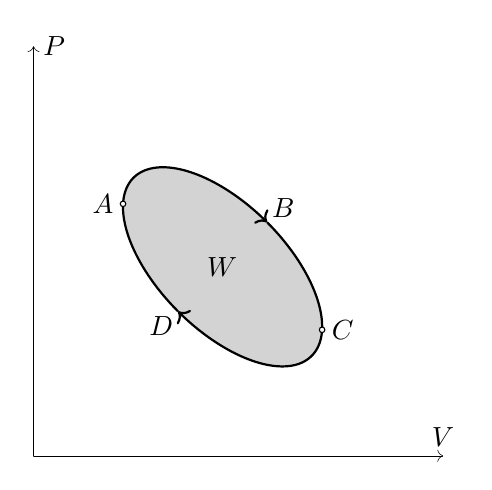
\begin{tikzpicture}[scale=0.8]
                    \tkzDefPoint(0,0){O}
                    \tkzDefPoint(6.5,0){X}
                    \tkzDefPoint(0,6.5){Y}
    
                    \tkzDrawSegment[->](O,X)
                    \tkzDrawSegment[->](O,Y)
    
                    \tkzLabelPoint[above](X){$V$}
                    \tkzLabelPoint[right](Y){$P$}

                    \fill[LightGray,rotate around={-45:(3,3)}] (3,3) ellipse (2 and 1);
                    \draw[smooth,thick,samples=100,domain=90:-90,->,rotate around={-45:(3,3)}] plot({2*cos(\x)+3},{1*sin(\x)+3});
                    \draw[smooth,thick,samples=100,domain=270:90,->,rotate around={-45:(3,3)}] plot({2*cos(\x)+3},{1*sin(\x)+3});

                    \tkzDefPoint(1.42,4.0){A}
                    \tkzDefPoint(3.6,3.6){B}
                    \tkzDefPoint(4.58,2.0){C}
                    \tkzDefPoint(2.4,2.4){D}

                    \tkzLabelPoint[left](A){$A$}
                    \tkzLabelPoint[above right=1pt](B){$B$}
                    \tkzLabelPoint[right](C){$C$}
                    \tkzLabelPoint[below left=1pt](D){$D$}

                    \tkzDrawPoint[fill=white](A)
                    \tkzDrawPoint[fill=white](C)

                    \tkzDefPoint(2.6,3){W}
                    \tkzLabelPoint[right](W){$W$}
                \end{tikzpicture}
            }\qquad\qquad
            \subfigure[逆循环过程]
            {
                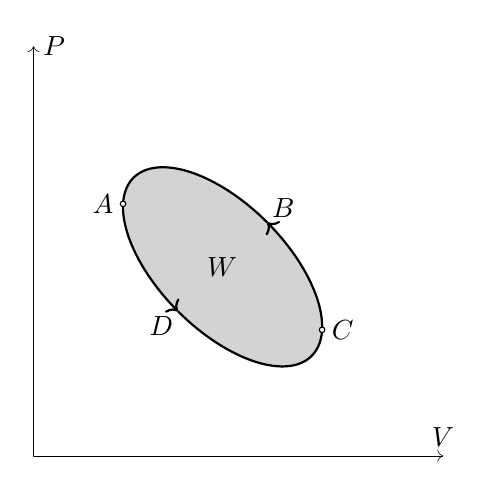
\begin{tikzpicture}[scale=0.8]
                    \tkzDefPoint(0,0){O}
                    \tkzDefPoint(6.5,0){X}
                    \tkzDefPoint(0,6.5){Y}
    
                    \tkzDrawSegment[->](O,X)
                    \tkzDrawSegment[->](O,Y)
    
                    \tkzLabelPoint[above](X){$V$}
                    \tkzLabelPoint[right](Y){$P$}

                    \fill[LightGray,rotate around={-45:(3,3)}] (3,3) ellipse (2 and 1);
                    \draw[smooth,thick,samples=100,domain=90:-90,<-,rotate around={-45:(3,3)}] plot({2*cos(\x)+3},{1*sin(\x)+3});
                    \draw[smooth,thick,samples=100,domain=270:90,<-,rotate around={-45:(3,3)}] plot({2*cos(\x)+3},{1*sin(\x)+3});

                    \tkzDefPoint(1.42,4.0){A}
                    \tkzDefPoint(3.6,3.6){B}
                    \tkzDefPoint(4.58,2.0){C}
                    \tkzDefPoint(2.4,2.4){D}

                    \tkzLabelPoint[left](A){$A$}
                    \tkzLabelPoint[above right=1pt](B){$B$}
                    \tkzLabelPoint[right](C){$C$}
                    \tkzLabelPoint[below left=1pt](D){$D$}

                    \tkzDrawPoint[fill=white](A)
                    \tkzDrawPoint[fill=white](C)

                    \tkzDefPoint(2.6,3){W}
                    \tkzLabelPoint[right](W){$W$}
                \end{tikzpicture}
            }
            \caption{循环过程}
        \end{center}
    \end{figure}\\
    循环过程中所做的功为曲线所包围的面积,经过一个循环内能不变。\\[3mm]
    循环过程为顺时针方向的称为正循环,工作物质作正循环的称为热机。\\[3mm]
    循环过程为逆时针方向的称为逆循环,工作物质作逆循环的称为热泵。\\[6mm]
    热机的工质在$A\rightarrow B\rightarrow C$的过程中吸收热量,体积膨胀,对外界做功。\\[3mm]
    热机的工质在$C\rightarrow D\rightarrow A$的过程中放出热量,体积压缩,受外界做功。\\[3mm]
    热机工质的膨胀中对外界做的功大于热机在压缩中受外界做的功,因此热机可以向外界做功。\\[3mm]
    热机中较为典型的包括蒸汽机和内燃机。\\[6mm]
    热泵的工质在$A\rightarrow D\rightarrow C$的过程中吸收热量,体积膨胀,对外界做功。\\[3mm]
    热泵的工质在$C\rightarrow B\rightarrow A$的过程中放出热量,体积压缩,受外界做功。\\[3mm]
    热泵工质的膨胀中对外界做的功小于热机在压缩中受外界做的功,因此热泵需要受外界做功。\\[3mm]
    热泵中较为典型的包括冷空调和暖空调。\\[6mm]

\newpage

\subsubsection{热机}
    热机可以向外界做功,从高温热源吸收热量,向低温热源放出热量,使得热源间的温度差减少。\\[3mm]
    热机是一种通过消耗高温热源和低温热源的温差,从而向外界做功的机械。\\[3mm]
    热机的工作原理可以用下图表示:\vspace{5pt}
    \begin{figure}[h]
        \begin{center}
            \begin{tikzpicture}[scale=1.0]
                \draw[very thick] (-5,+3.5) rectangle (5,+2.5);
                \node at(0,+3.0) {高温热源$T_1$};

                \draw[very thick] (-5,-3.5) rectangle (5,-2.5);
                \node at(0,-3.0) {低温热源$T_2$};

                \draw[very thick] (0,0) ellipse (1.3 and 1.0);
                \node at(0,0){工作物质};

                \tkzDefPoint(0,+2.5){Qh1}
                \tkzDefPoint(0,+1.0){Qh2}
                \tkzDefPoint(0,-2.5){Qc1}
                \tkzDefPoint(0,-1.0){Qc2}
                \tkzDefPoint(1.3,0){W1}
                \tkzDefPoint(2.0,0){W2}

                \tkzDrawSegment[-{>[scale=2]}](Qh1,Qh2)
                \tkzDrawSegment[-{>[scale=2]}](Qc2,Qc1)
                \tkzDrawSegment[-{>[scale=2]}](W1,W2)

                \tkzLabelSegment[right](Qh1,Qh2){$Q_1$}
                \tkzLabelSegment[right](Qc1,Qc2){$Q_2$}
                \tkzLabelPoint[right](W2){$W=Q_1-Q_2$}
            \end{tikzpicture}
            \caption{热机的工作原理}
        \end{center}
    \end{figure}\\
    热机可以用于对外做功,例如蒸汽机用于做功驱动机械。\\[3mm]
    热机做功时,将蒸汽作为高温热源,将空气作为低温热源,通过热机的工作从而做功驱动机械。\\[6mm]
    热机的一个重要指标是热机效率$\eta$:
    \begin{large}
        \begin{align*}
            &\eta=\frac{W}{Q_1}=\frac{Q_1-Q_2}{Q_1}\\[6mm]
            &\eta=\frac{W}{Q_1}=1-\frac{Q_2}{Q_1}
        \end{align*}
    \end{large}\\
    热机效率$\eta$定义为工质输出的功$W$与高温热源吸收热量$Q_1$的比值。\\[3mm]

\newpage

\subsubsection{热泵}
    热泵需要受外界做功,从低温热源吸收热量,向高温热源放出热量,使得热源间的温度差增加。\\[3mm]
    热泵是一种通过受外界做功,从而增大高温热源和低温热源的温差的机械。\\[3mm]
    热泵的工作原理可以用下图表示:\vspace{5pt}
    \begin{figure}[h]
        \begin{center}
            \begin{tikzpicture}[scale=1.0]
                \draw[very thick] (-5,+3.5) rectangle (5,+2.5);
                \node at(0,+3.0) {高温热源$T_1$};

                \draw[very thick] (-5,-3.5) rectangle (5,-2.5);
                \node at(0,-3.0) {低温热源$T_2$};

                \draw[very thick] (0,0) ellipse (1.3 and 1.0);
                \node at(0,0){工作物质};

                \tkzDefPoint(0,+2.5){Qh1}
                \tkzDefPoint(0,+1.0){Qh2}
                \tkzDefPoint(0,-2.5){Qc1}
                \tkzDefPoint(0,-1.0){Qc2}
                \tkzDefPoint(1.3,0){W1}
                \tkzDefPoint(2.0,0){W2}

                \tkzDrawSegment[-{>[scale=2]}](Qh2,Qh1)
                \tkzDrawSegment[-{>[scale=2]}](Qc1,Qc2)
                \tkzDrawSegment[-{>[scale=2]}](W2,W1)

                \tkzLabelSegment[right](Qh1,Qh2){$Q_1$}
                \tkzLabelSegment[right](Qc1,Qc2){$Q_2$}
                \tkzLabelPoint[right](W2){$W=Q_1-Q_2$}
            \end{tikzpicture}
            \caption{热泵的工作原理}
        \end{center}
    \end{figure}\\
    热泵可以用于供热或制冷,例如热空调用于供热,例如冷空调用于制冷。\\[3mm]
    热泵供热时,将室内作为高温热源,将室外作为低温热源,通过热泵的工作使得室内温度更高。\\[3mm]
    热泵制冷时,将室内作为低温热源,将室外作为高温热源,通过热泵的工作使得室内温度更低。\\[6mm]
    热泵制冷时的一个重要指标是热泵制冷效能$w_c$:
    \begin{large}
        \begin{equation*}
            w_c=\frac{Q_2}{W}=\frac{Q_2}{Q_1-Q_2}
        \end{equation*}
    \end{large}\\
    热泵供暖时的一个重要指标是热泵供暖效能$w_h$:
    \begin{large}
        \begin{equation*}
            w_h=\frac{Q_1}{W}=\frac{Q_1}{Q_1-Q_2}
        \end{equation*}
    \end{large}\\
    热泵制冷效能$w_c\,$定义为从低温热源吸收的热量$Q_2$和工质输入的功$W$的比值。\\[3mm]
    热泵供暖效能$w_h$定义为向高温热源放出的热量$Q_1$和工质输入的功$W$的比值。

\newpage

\subsubsection{卡诺正循环}
    \setcounter{equation}{0}
    卡诺正循环以理想气体为工质,由两个等温过程和两个绝热过程组成的循环过程。\\[3mm]
    卡诺正循环可以用$P-V$图上的封闭曲线表示:
    \begin{figure}[h]
        \begin{center}
            \begin{tikzpicture}[scale=1.0]
                \tkzDefPoint(0,0){O}
                \tkzDefPoint(9.5.0,0){X}
                \tkzDefPoint(0,8.5){Y}

                \tkzDrawSegment[->](O,X)
                \tkzDrawSegment[->](O,Y)

                \tkzLabelPoint[above](X){$V$}
                \tkzLabelPoint[right](Y){$P$}

                \fill [fill=LightGray] [domain = 1.334:2.449,smooth] plot (\x,10.906/\x^1.667) -- (3,3) [domain = 3.000:1.334, smooth] -- plot (\x,9/\x) -- cycle;
                \fill [fill=LightGray] [domain = 3.000:5.541,smooth] plot (\x,18.789/\x^1.667) -- (3,3) [domain = 5.541:2.449, smooth] -- plot (\x,6/\x) -- cycle;

                \draw[smooth,thick,samples=100,domain=1.334:2.167,->] plot(\x,9/\x);
                \draw[smooth,thick,samples=100,domain=2.167:3.000] plot(\x,9/\x);

                \draw[smooth,thick,samples=100,domain=3.000:4.271,->] plot(\x,18.789/\x^1.667);
                \draw[smooth,thick,samples=100,domain=4.271:5.541] plot(\x,18.789/\x^1.667);

                \draw[smooth,thick,samples=100,domain=2.449:3.600,-<] plot(\x,6/\x);
                \draw[smooth,thick,samples=100,domain=3.600:5.541] plot(\x,6/\x);

                \draw[smooth,thick,samples=100,domain=1.334:1.892,-<] plot(\x,10.906/\x^1.667);
                \draw[smooth,thick,samples=100,domain=1.892:2.449] plot(\x,10.906/\x^1.667);

                \draw[smooth,thick,samples=100,domain=1.15:7.0,dashed] plot(\x,9/\x);
                \draw[smooth,thick,samples=100,domain=0.90:8.0,dashed] plot(\x,6/\x);

                \tkzDefPoint(1.334,6.746){A}
                \tkzDefPoint(3.000,3.000){B}
                \tkzDefPoint(5.541,1.083){C}
                \tkzDefPoint(2.449,2.449){D}

                \tkzDefPoint(1.15,7.826){T1}
                \tkzDefPoint(0.90,6.666){T2}

                \tkzDrawPoints[fill=white](A,B,C,D)

                \tkzLabelPoint[right](A){$A(P_1,V_1,T_1)$}
                \tkzLabelPoint[right](B){$B(P_2,V_2,T_1)$}
                \tkzLabelPoint[below left](C){$C(P_3,V_3,T_2)$}
                \tkzLabelPoint[below left](D){$D(P_4,V_4,T_2)$}
                \tkzLabelPoint[left](T1){$T_1$}
                \tkzLabelPoint[left](T2){$T_2$}
            \end{tikzpicture}
            \caption{卡诺正循环}
        \end{center}
    \end{figure}\\
    卡诺正循环分为四个过程:\\[3mm]
    1.等温膨胀过程$A-B$,温度不变($T_1\rightarrow T_1$),体积增大($V_1\rightarrow V_2$)。\\[3mm]
    2.绝热膨胀过程$B-C$,温度降低($T_1\rightarrow T_2$),体积增大($V_2\rightarrow V_1$)。\\[3mm]
    3.等温压缩过程$C-D$,温度不变($T_2\rightarrow T_2$),体积减小($V_3\rightarrow V_3$)。\\[3mm]
    4.绝热压缩过程$D-A$\hspace{0.4pt},温度升高($T_2\rightarrow T_1$),体积减小($V_4\rightarrow V_1$)。\\[6mm]
    卡诺正循环工作于温度为$T_1$的高温热源和温度为$T_2$的低温热源:\\[3mm]
    1.等温膨胀过程$A-B$,工质从温度\hspace{4pt}$T_1$\hspace{4pt}的高温热源吸收热量$Q_1$,能量用于对外界做功。\\[3mm]
    2.绝热膨胀过程$B-C$,工质绝热,内能减少使得温度下降至$T_2$,能量用于对外界做功。\\[3mm]
    3.等温压缩过程$C-D$,工质向温度\hspace{4pt}$T_2$\hspace{4pt}的低温热源放出热量$Q_2$,能量来自受外界做功。\\[3mm]
    4.绝热压缩过程$D-A$\hspace{0.4pt},工质绝热,内能增加使得温度升高至$T_1$,能量来自受外界做功。\\[5mm]

\newpage

    卡诺正循环对应的机械称为卡诺热机,现在我们研究卡诺热机的效率。\\[3mm]
    在等温膨胀$A(V_1,T_1)-B(V_2,T_1)$中,从高温热源吸收的热量为:\vspace{5pt}
    \begin{align}
        &Q_1=+\left(\frac{m}{M}\cdot R\cdot T_1\cdot\ln{\frac{V_2}{V_1}}\right)=\frac{m}{M}\cdot R\cdot T_1\cdot\ln{\frac{V_2}{V_1}}
    \end{align}\\
    在等温压缩$C(V_3,T_2)-D(V_4,T_2)$中,向低温热源放出的热量为:\vspace{5pt}
    \begin{align}
        &Q_2=-\left(\frac{m}{M}\cdot R\cdot T_2\cdot\ln{\frac{V_4}{V_3}}\right)=\frac{m}{M}\cdot R\cdot T_1\cdot\ln{\frac{V_3}{V_4}}
    \end{align}\\
    对绝热膨胀$B(V_2,T_1)-C(V_3,T_2)$使用绝热方程:
    \begin{align}
        &T_1\cdot V_2^{\gamma-1}=T_2\cdot V_3^{\gamma-1}
    \end{align}\\
    对绝热压缩$D(V_4,T_2)-A(V_1,T_1)$使用绝热方程:
    \begin{align}
        &T_1\cdot V_1^{\gamma-1}=T_2\cdot V_4^{\gamma-1}
    \end{align}\\
    将两个绝热方程作比可以得到:
    \begin{align}
        \frac{T_1\cdot V_2^{\gamma-1}}{T_1\cdot V_1^{\gamma-1}}=\frac{T_2\cdot V_3^{\gamma-1}}{T_2\cdot V_4^{\gamma-1}}~~\Rightarrow~~\frac{V_2}{V_1}&=\frac{V_3}{V_4}
    \end{align}\\
    将吸收和放出的热量作比可得:
    \begin{align}
        &\frac{Q_1}{Q_2}=\frac{\dfrac{m}{M}\cdot R\cdot T_1-\ln{\dfrac{V_2}{V_1}}}{\dfrac{m}{M}\cdot R\cdot T_2-\ln{\dfrac{V_3}{V_4}}}=\frac{T_1}{T_2}
    \end{align}\\
    卡诺热机的效率的计算公式:
    \begin{large}
        \begin{align*}
            &\eta_C=\frac{T_1-T_2}{T_1}\\[4mm]
            &\eta_C=1-\frac{T_2}{T_1}
        \end{align*}
    \end{large}\\
    卡诺热机的效率$\eta_C$只和高温热源和低温热源的温度有关。\\[3mm]
    卡诺热机的效率$\eta_C$的计算公式指出,温差越大,低温热源的温度越低,效率越高。\\[3mm]
    由于低温热源的温度$T_2\neq 0$,故卡诺热机的效率$\eta<1$。

\newpage

\subsubsection{卡诺逆循环}
    \setcounter{equation}{0}
    卡诺逆循环以理想气体为工质,由两个等温过程和两个绝热过程组成的循环过程。\\[3mm]
    卡诺逆循环可以用$P-V$图上的封闭曲线表示:
    \begin{figure}[h]
        \begin{center}
            \begin{tikzpicture}[scale=1.0]
                \tkzDefPoint(0,0){O}
                \tkzDefPoint(9.5.0,0){X}
                \tkzDefPoint(0,8.5){Y}

                \tkzDrawSegment[->](O,X)
                \tkzDrawSegment[->](O,Y)

                \tkzLabelPoint[above](X){$V$}
                \tkzLabelPoint[right](Y){$P$}

                \fill [fill=LightGray] [domain = 1.334:2.449,smooth] plot (\x,10.906/\x^1.667) -- (3,3) [domain = 3.000:1.334, smooth] -- plot (\x,9/\x) -- cycle;
                \fill [fill=LightGray] [domain = 3.000:5.541,smooth] plot (\x,18.789/\x^1.667) -- (3,3) [domain = 5.541:2.449, smooth] -- plot (\x,6/\x) -- cycle;

                \draw[smooth,thick,samples=100,domain=1.334:2.167,-<] plot(\x,9/\x);
                \draw[smooth,thick,samples=100,domain=2.167:3.000] plot(\x,9/\x);

                \draw[smooth,thick,samples=100,domain=3.000:4.271,-<] plot(\x,18.789/\x^1.667);
                \draw[smooth,thick,samples=100,domain=4.271:5.541] plot(\x,18.789/\x^1.667);

                \draw[smooth,thick,samples=100,domain=2.449:3.600,->] plot(\x,6/\x);
                \draw[smooth,thick,samples=100,domain=3.600:5.541] plot(\x,6/\x);

                \draw[smooth,thick,samples=100,domain=1.334:1.892,->] plot(\x,10.906/\x^1.667);
                \draw[smooth,thick,samples=100,domain=1.892:2.449] plot(\x,10.906/\x^1.667);

                \draw[smooth,thick,samples=100,domain=1.15:7.0,dashed] plot(\x,9/\x);
                \draw[smooth,thick,samples=100,domain=0.90:8.0,dashed] plot(\x,6/\x);

                \tkzDefPoint(1.334,6.746){A}
                \tkzDefPoint(3.000,3.000){B}
                \tkzDefPoint(5.541,1.083){C}
                \tkzDefPoint(2.449,2.449){D}

                \tkzDefPoint(1.15,7.826){T1}
                \tkzDefPoint(0.90,6.666){T2}

                \tkzDrawPoints[fill=white](A,B,C,D)

                \tkzLabelPoint[right](A){$A(P_1,V_1,T_1)$}
                \tkzLabelPoint[right](B){$B(P_2,V_2,T_1)$}
                \tkzLabelPoint[below left](C){$C(P_3,V_3,T_2)$}
                \tkzLabelPoint[below left](D){$D(P_4,V_4,T_2)$}
                \tkzLabelPoint[left](T1){$T_1$}
                \tkzLabelPoint[left](T2){$T_2$}
            \end{tikzpicture}
            \caption{卡诺逆循环}
        \end{center}
    \end{figure}\\
    卡诺逆循环分为四个过程:\\[3mm]
    1.绝热膨胀过程$A-D$\hspace{0.4pt},温度降低($T_1\rightarrow T_2$),体积增大($V_1\rightarrow V_4$)。\\[3mm]
    2.等温膨胀过程$D-C$,温度不变($T_2\rightarrow T_2$),体积增大($V_4\rightarrow V_3$)。\\[3mm]
    3.绝热压缩过程$C-B$,温度升高($T_2\rightarrow T_1$),体积减小($V_3\rightarrow V_2$)。\\[3mm]
    4.等温压缩过程$B-A$,温度不变($T_1\rightarrow T_1$),体积减小($V_2\rightarrow V_1$)。\\[6mm]
    卡诺逆循环工作于温度为$T_1$的高温热源和温度为$T_2$的低温热源:\\[3mm]
    1.绝热膨胀过程$A-D$,工质绝热,内能减少使得温度下降至$T_2$,能量用于对外界做功。\\[3mm]
    2.等温膨胀过程$D-C$,工质从温度\hspace{4pt}$T_2$\hspace{4pt}的低温热源吸收热量$Q_2$,能量用于对外界做功。\\[3mm]
    3.绝热压缩过程$C-B$\hspace{0.4pt},工质绝热,内能增加使得温度升高至$T_1$,能量来自受外界做功。\\[3mm]
    4.等温压缩过程$B-A$,工质向温度\hspace{4pt}$T_1$\hspace{4pt}的高温热源放出热量$Q_1$,能量来自受外界做功。
    

\newpage

    卡诺逆循环对应的机械称为卡诺热泵,现在我们研究卡诺热泵的效能。\\[3mm]
    在等温膨胀$D(V_4,T_2)-C(V_3,T_2)$中,从低温热源吸收的热量为:\vspace{5pt}
    \begin{align}
        &Q_2=+\left(\frac{m}{M}\cdot R\cdot T_2\cdot\ln{\frac{V_3}{V_4}}\right)=\frac{m}{M}\cdot R\cdot T_2\cdot\ln{\frac{V_3}{V_4}}
    \end{align}\\
    在等温压缩$B(V_2,T_1)-A(V_1,T_1)$中,向高温热源放出的热量为:\vspace{5pt}
    \begin{align}
        &Q_1=-\left(\frac{m}{M}\cdot R\cdot T_1\cdot\ln{\frac{V_1}{V_2}}\right)=\frac{m}{M}\cdot R\cdot T_1\cdot\ln{\frac{V_2}{V_1}}
    \end{align}\\
    对绝热膨胀$A(V_1,T_1)-D(V_4,T_2)$使用绝热方程:
    \begin{align}
        &T_1\cdot V_1^{\gamma-1}=T_2\cdot V_4^{\gamma-1}
    \end{align}\\
    对绝热压缩$C(V_3,T_2)-B(V_2,T_1)$使用绝热方程:
    \begin{align}
        &T_1\cdot V_2^{\gamma-1}=T_2\cdot V_3^{\gamma-1}
    \end{align}\\
    将两个绝热方程作比可以得到:
    \begin{align}
        \frac{T_1\cdot V_2^{\gamma-1}}{T_1\cdot V_1^{\gamma-1}}=\frac{T_2\cdot V_3^{\gamma-1}}{T_2\cdot V_4^{\gamma-1}}~~\Rightarrow~~\frac{V_2}{V_1}&=\frac{V_3}{V_4}
    \end{align}\\
    将放出和吸收的热量作比可得:
    \begin{align}
        &\frac{Q_1}{Q_2}=\frac{\dfrac{m}{M}\cdot R\cdot T_1-\ln{\dfrac{V_2}{V_1}}}{\dfrac{m}{M}\cdot R\cdot T_2-\ln{\dfrac{V_3}{V_4}}}=\frac{T_1}{T_2}
    \end{align}\\
    卡诺热泵的效能的计算公式:
    \begin{large}
        \begin{align*}
            &w_{C_h}=\frac{T_1}{T_1-T_2}\\[4mm]
            &w_{C_c}=\frac{T_2}{T_1-T_2}
        \end{align*}
    \end{large}\\
    卡诺热泵的效能$w$只和高温热源和低温热源的温度有关。\\[3mm]
    卡诺热泵的供热效能$w_{C_h}$的计算公式指出,温差越大,高温热源的温度越低,供热效能越低。\\[3mm]
    卡诺热泵的制冷效能$w_{C_c}$的计算公式指出,温差越大,低温热源的温度越低,制冷效能越低。\\[3mm]
    由于低温热源的温度$T_2\neq 0$,故卡诺热泵的供热效能$w_{C_h}>1$。

\newpage

\subsection{热力学第二定律}
    \setcounter{equation}{0}
    \textbf{热力学第二定律(克劳修斯):}不可能把热量从低温物体传递到高温物体,而不产生其他影响。\\[3mm]
    热力学第二定律的克劳修斯表述指出,自发的热量传递具有不可逆性,只能由高温到低温。\\[3mm]
    热泵虽然可以使得热量从低温物体传递到高温物体,但是却需要通过热泵额外做功才能实现。\\[12mm]
    \textbf{热力学第二定律(开尔文):}不可能从单一热源吸收热量,使之完全变为功而不产生其他影响。\\[3mm]
    热力学第二定律的开尔文表述指出,功可以自发的转变为热,热却不可以自发的转变为功。\\[3mm]
    热力学第二定律的开尔文表述同时说明了热机的效率$\eta$不可能达到$100\%$。\\[6mm]
    根据热机效率的计算公式:
    \begin{align}
        \eta=1-\frac{Q_2}{Q_1}
    \end{align}\\
    观察该公式可以发现,假如向低温热源放出的热量$Q_2=0$,那么热机的效率就可以达到$100\%$。\\[3mm]
    然而这是不可能实现的,因为卡诺从理论上证明了卡诺热机在温差一定时具有最高的效率。\\[8mm]
    根据卡诺热机效率的公式:
    \begin{align}
        \eta_C=1-\frac{T_2}{T_1}
    \end{align}\\
    观察该公式可以发现,只有当低温热源的温度为$T_2=0$,那么卡诺热机的效率才能达到$100\%$。\\[3mm]
    但是绝对零度是不可能达到的,这就说明了热机不可能使热完全转化为功。\\[12mm]
    热力学第一定律和热力学第二定律是缺一不可的:\\[3mm]
    1.热力学第一定律说明了任何过程必须满足能量守恒定律。\\[3mm]
    2.热力学第二定律说明了并非所有满足能量守恒定理的过程均能实现。

\subsubsection{第二类永动机}
    第二类永动机指的是可以从单一热源吸收热量并完全转变为功而不产生其他影响的机器。\\[3mm]
    第二类永动机违背了热力学第二定律的开尔文表述,因此不可能实现。

\newpage

\part{电}

\newpage

\section{真空中静电场}

\subsection{电荷}
    电荷只有两种类型:负电荷,正电荷。\\[3mm]
    1.负电荷,用$-$表示,例如电子所带的电荷就为负电荷。\\[3mm]
    2.正电荷,用$+$表示,例如质子所带的电荷就为正电荷。\\[3mm]
    例如丝绸和玻璃棒摩擦会发生电荷的转移,丝绸带负电荷,玻璃棒带正电荷。\\[3mm]
    例如毛皮和橡胶棒摩擦会发生电荷的转移,毛皮带正电荷,橡胶棒带负电荷。\\[6mm]
    电荷量衡量了物体所带电荷数量的多少,通常用字母$Q$表示,是一个标量,单位是\si{C}。\\[3mm]
    电荷量的单位库伦定义如下:
    \begin{large}
        \begin{equation*}
            C=A\cdot s
        \end{equation*}
    \end{large}\\
    电荷量在不引起误解的情况下,也可以简称为电荷或电量。\\[3mm]
    点电荷是一种理想模型,只具有质量和电荷量,没有大小,没有形状。\\[3mm]
    点电荷通常在带电体的大小远远小于带电体的距离时使用,此时大小形状相较于距离可以忽略。\\[6mm]
    \textbf{电荷守恒定律:}在一个孤立系统中,电荷既不能被创造,电荷也不能被消灭,只能从一个物体转移到另一个物体,
    或者从物体的一个部分转移到另一个部分。\\[3mm]
    电荷守恒定律描述了电荷在一切宏观过程和微观过程中所遵循的基本规律。\vspace{5pt}

\subsubsection{元电荷}
    实验表明,物体所带电荷量的值是不连续的,物体所带电荷量总是某一值的整数倍。\\[3mm]
    研究表明,这一数值为质子或电子所带电荷量的大小,称之为元电荷或基本电荷。\\[3mm]
    元电荷的数值为:
    \begin{large}
        \begin{equation*}
            e=1.602\times 10^{-19}\si{C}
        \end{equation*}
    \end{large}\\
    元电荷的数值由密立根通过密立根油滴实验测定。\\[3mm]
    如果用元电荷$e$表示质子的电荷量,那么质子的电荷量可以写作$+e$。\\[3mm]
    如果用元电荷$e$表示电子的电荷量,那么电子的电荷量可以写作$-e$。

\newpage

\subsection{电场}
    电荷间有相互作用力,同性电荷相互排斥,异性电荷相互吸引。\\[3mm]
    电荷不需要相互接触就可以有作用力,但是这种作用实际并不是超距的。\\[3mm]
    电荷间的相互作用是通过电场实现的:\vspace{5pt}
    \begin{figure}[h]
        \begin{center}
            \begin{tikzpicture}[scale=1.1]
                \tkzDefPoint(0,+5.0){Q1}
                \tkzDefPoint(0,-5.0){Q2}

                \tkzDefShiftPoint[Q1](0,-0.9){Q1d}
                \tkzDefShiftPoint[Q2](0,+0.9){Q2u}

                \tkzDefPoint(0,0){E}

                \tkzDefShiftPoint[E](0,-0.5){Ed}
                \tkzDefShiftPoint[E](0,+0.5){Eu}

                \tkzDrawCircle[R](Q1,0.9cm)
                \tkzDrawCircle[R](Q2,0.9cm)

                \draw (-1.0,+0.5) rectangle (+1.0,-0.5);

                \node at (Q1) {电荷$Q_1$};
                \node at (Q2) {电荷$Q_2$};

                \node at (E) {电场};

                \tkzDrawSegment[thick,<->](Q1d,Eu)
                \tkzDrawSegment[thick,<->](Q2u,Ed)
            \end{tikzpicture}
            \caption{电荷通过电场传递相互作用力}
        \end{center}
    \end{figure}\\
    电荷在其周围会激发电场,由静止电荷激发的电场称为静电场。\\[3mm]
    电场是一种特殊但客观存在的物质,因此电场也具有能量和动量。\\[3mm]

\newpage

\subsection{电场力}
    电场力衡量了电荷在电场中受到的力,通常用符号$\veb{F}$表示,是一个矢量,单位是\si{N}。\\[3mm]
    电场力的计算公式(矢量形式):
    \begin{large}
        \begin{equation*}
            \veb{F}=\frac{1}{4\pi\cdot\varepsilon_0}\cdot\frac{Q_1\cdot Q_2}{r^2}\cdot\veb{r_0}
        \end{equation*}
    \end{large}\\
    电场力的计算公式(标量形式):
    \begin{large}
        \begin{equation*}
            F=\frac{1}{4\pi\cdot\varepsilon_0}\cdot\frac{Q_1\cdot Q_2}{r^2}
        \end{equation*}
    \end{large}\\
    该结论也被称为库伦定律。\\[3mm]
    其中$\varepsilon_0$为真空电容率,其取值为$\varepsilon_0=8.85\times 10^{-12}$~\si{C^2/(N\cdot m^2)}。\\[3mm]
    其中$Q_1,Q_2$代表了施力电荷和受力电荷,而$\veb{r_0}$代表施力电荷和受力电荷的位矢的单位矢量。\\[6mm]
    当两个电荷同号时的电场力:
    \begin{figure}[h]
        \begin{center}
            \begin{tikzpicture}[scale=1.0]
                \tkzDefPoint(-3,0){Q1}
                \tkzDefPoint(+3,0){Q2}

                \tkzDefShiftPoint[Q1](-2.0,0){L1}
                \tkzDefShiftPoint[Q2](+2.0,0){L2}

                \tkzDefShiftPoint[Q1](+0.3,0){RS}
                \tkzDefShiftPoint[Q1](+1.3,0){RE}

                \tkzDefShiftPoint[Q2](+0.3,0){FS}
                \tkzDefShiftPoint[Q2](+1.3,0){FE}

                \tkzDefShiftPoint[Q1](0,-0.3){R1A}
                \tkzDefShiftPoint[Q1](0,-0.5){R1B}
                \tkzDefShiftPoint[Q1](0,-0.7){R1C}

                \tkzDefShiftPoint[Q2](0,-0.3){R2A}
                \tkzDefShiftPoint[Q2](0,-0.5){R2B}
                \tkzDefShiftPoint[Q2](0,-0.7){R2C}

                \tkzDrawSegment[dashed](L1,L2)
                \tkzDrawSegment(R1A,R1C)
                \tkzDrawSegment(R2A,R2C)

                \tkzDrawSegment[<->](R1B,R2B)

                \tkzDrawSegment[-latex](RS,RE)
                \tkzDrawSegment[-latex](FS,FE)

                \tkzDrawCircle[fill=white](Q1,RS)
                \tkzDrawCircle[fill=white](Q2,FS)

                \tkzLabelSegment[below](R1B,R2B){$r$}
                \tkzLabelPoint[above=8pt](Q1){$Q_1$}
                \tkzLabelPoint[above=8pt](Q2){$Q_2$}

                \tkzLabelPoint[above](RE){$\veb{r_0}$}
                \tkzLabelPoint[above](FE){$\veb{F}$}

                \node at (Q1) {$+$};
                \node at (Q2) {$+$};
            \end{tikzpicture}
            \caption{两个电荷同号时的受力情况}
        \end{center}
    \end{figure}\\
    当两个电荷异号时的电场力:
    \begin{figure}[h]
        \begin{center}
            \begin{tikzpicture}[scale=1.0]
                \tkzDefPoint(-3,0){Q1}
                \tkzDefPoint(+3,0){Q2}

                \tkzDefShiftPoint[Q1](-2.0,0){L1}
                \tkzDefShiftPoint[Q2](+2.0,0){L2}

                \tkzDefShiftPoint[Q1](+0.3,0){RS}
                \tkzDefShiftPoint[Q1](+1.3,0){RE}

                \tkzDefShiftPoint[Q2](-0.3,0){FS}
                \tkzDefShiftPoint[Q2](-1.3,0){FE}

                \tkzDefShiftPoint[Q1](0,-0.3){R1A}
                \tkzDefShiftPoint[Q1](0,-0.5){R1B}
                \tkzDefShiftPoint[Q1](0,-0.7){R1C}

                \tkzDefShiftPoint[Q2](0,-0.3){R2A}
                \tkzDefShiftPoint[Q2](0,-0.5){R2B}
                \tkzDefShiftPoint[Q2](0,-0.7){R2C}

                \tkzDrawSegment[dashed](L1,L2)
                \tkzDrawSegment(R1A,R1C)
                \tkzDrawSegment(R2A,R2C)

                \tkzDrawSegment[<->](R1B,R2B)

                \tkzDrawSegment[-latex](RS,RE)
                \tkzDrawSegment[-latex](FS,FE)

                \tkzDrawCircle[fill=white](Q1,RS)
                \tkzDrawCircle[fill=white](Q2,FS)

                \tkzLabelSegment[below](R1B,R2B){$r$}
                \tkzLabelPoint[above=8pt](Q1){$Q_1$}
                \tkzLabelPoint[above=8pt](Q2){$Q_2$}

                \tkzLabelPoint[above](RE){$\veb{r_0}$}
                \tkzLabelPoint[above](FE){$\veb{F}$}

                \node at (Q1) {$-$};
                \node at (Q2) {$+$};
            \end{tikzpicture}
            \caption{两个电荷同号时的受力情况}
        \end{center}
    \end{figure}\\
    第一种情况中,电荷量的乘积$Q_1\cdot Q_2$为正值,故电场力$\veb{F}$的方向和$r_0$方向相同。\\[3mm]
    第二种情况中,电荷量的乘积$Q_1\cdot Q_2$为负值,故电场力$\veb{F}$的方向和$r_0$方向相反。\\[6mm]
    库伦定律中也可以引入一比例系数$k=\dfrac{1}{4\pi\cdot\varepsilon_0}=8.98\times 10^9~\si{(N\cdot m^2)/C^2}$。\\[3mm]
    库伦定律会因此变得更为简单,但这会使更为常用的导出公式变得复杂,故通常不使用该系数。

\subsection{电场强度}
    \setcounter{equation}{0}
    电场强度衡量了电场的强弱,通常用符号$\veb{E}$表示,是一个矢量,单位是\si{N/C}。\\[3mm]
    电场强度的计算公式(矢量形式):
    \begin{large}
        \begin{equation*}
            \veb{E}=\frac{1}{4\pi\cdot\varepsilon_0}\cdot\frac{Q_1}{r^2}\cdot\veb{r_0}
        \end{equation*}
    \end{large}\\
    电场强度的计算公式(标量形式):
    \begin{large}
        \begin{equation*}
            E=\frac{1}{4\pi\cdot\varepsilon_0}\cdot\frac{Q_1}{r^2}
        \end{equation*}
    \end{large}\\
    其中$Q_1$代表场源电荷,而$\veb{r_0}$代表场源指向场点的位矢的单位矢量。\\[3mm]
    其中$Q_2$代表试验电荷,而$\veb{F}$为试验电荷在场源电荷中某一处受到的电场力。\\[3mm]
    试验电荷的电荷量十分的小,以至于其自身产生的电场相较于场源电荷的电场可以忽略。\\[6mm]
    电场强度定义为单位电荷量的试验电荷在电场中所受到的电场力。\\[3mm]
    电场强度的计算公式的推导如下:
    \begin{align}
        &\veb{E}=\frac{\veb{F}}{Q_2}=\frac{1}{4\pi\cdot\varepsilon_0}\cdot\frac{Q_1}{r^2}\cdot\veb{r_0}
    \end{align}\\
    当场源电荷为正电荷时的电场强度:
    \begin{figure}[h!]
        \begin{center}
            \begin{tikzpicture}[scale=1.0]
                \tkzDefPoint(-3,0){Q1}
                \tkzDefPoint(+3,0){Q2}

                \tkzDefShiftPoint[Q1](-2.0,0){L1}
                \tkzDefShiftPoint[Q2](+2.0,0){L2}

                \tkzDefShiftPoint[Q1](+0.3,0){RS}
                \tkzDefShiftPoint[Q1](+1.3,0){RE}

                \tkzDefShiftPoint[Q2](+0.0,0){FS}
                \tkzDefShiftPoint[Q2](+1.3,0){FE}

                \tkzDefShiftPoint[Q1](0,-0.3){R1A}
                \tkzDefShiftPoint[Q1](0,-0.5){R1B}
                \tkzDefShiftPoint[Q1](0,-0.7){R1C}

                \tkzDefShiftPoint[Q2](0,-0.3){R2A}
                \tkzDefShiftPoint[Q2](0,-0.5){R2B}
                \tkzDefShiftPoint[Q2](0,-0.7){R2C}

                \tkzDrawSegment[dashed](L1,L2)
                \tkzDrawSegment(R1A,R1C)
                \tkzDrawSegment(Q2,R2C)

                \tkzDrawSegment[<->](R1B,R2B)

                \tkzDrawSegment[-latex](RS,RE)
                \tkzDrawSegment[-latex](FS,FE)

                \tkzDrawCircle[fill=white](Q1,RS)
                \tkzDrawPoint[fill=white](Q2)

                \tkzLabelSegment[below](R1B,R2B){$r$}
                \tkzLabelPoint[above=8pt](Q1){$Q_1$}

                \tkzLabelPoint[above](RE){$\veb{r_0}$}
                \tkzLabelPoint[above](FE){$\veb{E}$}

                \node at (Q1) {$+$};
            \end{tikzpicture}
            \caption{场源电荷为正电荷时的电场强度}
        \end{center}
    \end{figure}\\
    当场源电荷为正电荷时的电场强度:
    \begin{figure}[h!]
        \begin{center}
            \begin{tikzpicture}[scale=1.0]
                \tkzDefPoint(-3,0){Q1}
                \tkzDefPoint(+3,0){Q2}

                \tkzDefShiftPoint[Q1](-2.0,0){L1}
                \tkzDefShiftPoint[Q2](+2.0,0){L2}

                \tkzDefShiftPoint[Q1](+0.3,0){RS}
                \tkzDefShiftPoint[Q1](+1.3,0){RE}

                \tkzDefShiftPoint[Q2](+0.0,0){FS}
                \tkzDefShiftPoint[Q2](-1.3,0){FE}

                \tkzDefShiftPoint[Q1](0,-0.3){R1A}
                \tkzDefShiftPoint[Q1](0,-0.5){R1B}
                \tkzDefShiftPoint[Q1](0,-0.7){R1C}

                \tkzDefShiftPoint[Q2](0,-0.3){R2A}
                \tkzDefShiftPoint[Q2](0,-0.5){R2B}
                \tkzDefShiftPoint[Q2](0,-0.7){R2C}

                \tkzDrawSegment[dashed](L1,L2)
                \tkzDrawSegment(R1A,R1C)
                \tkzDrawSegment(Q2,R2C)

                \tkzDrawSegment[<->](R1B,R2B)

                \tkzDrawSegment[-latex](RS,RE)
                \tkzDrawSegment[-latex](FS,FE)

                \tkzDrawCircle[fill=white](Q1,RS)
                \tkzDrawPoint[fill=white](Q2)

                \tkzLabelSegment[below](R1B,R2B){$r$}
                \tkzLabelPoint[above=8pt](Q1){$Q_1$}

                \tkzLabelPoint[above](RE){$\veb{r_0}$}
                \tkzLabelPoint[above](FE){$\veb{E}$}

                \node at (Q1) {$-$};
            \end{tikzpicture}
            \caption{场源电荷为正电荷时的电场强度}
        \end{center}
    \end{figure}\\
    第一种情况中,场源电荷的电荷量的乘积$Q_1$为正值,故电场强度$\veb{E}$的方向和$r_0$方向相同。\\[3mm]
    第二种情况中,场源电荷的电荷量的乘积$Q_1$为负值,故电场强度$\veb{E}$的方向和$r_0$方向相反。

\newpage

\subsubsection{电场强度的迭加原理}
    \setcounter{equation}{0}
    \textbf{电场强度的迭加原理:}点电荷系在某一场点产生的电场强度,等于该点电荷系中的每一个电荷,
    在其单独存在时,分别在该场点产生的电场强度的矢量和。\\[3mm]
    电场强度的迭加原理的数学表达:
    \begin{large}
        \begin{equation*}
            \veb{E}=\sum_{i=1}^{n}\veb{E_i}=\sum_{i=1}^{n}\frac{1}{4\pi\cdot\varepsilon_0}\cdot\frac{Q_i}{r_i^2}\cdot\veb{r_{0_i}}
        \end{equation*}
    \end{large}\\
    设点电荷系由$n$个点电荷$Q_1\sim Q_n$组成,使用的试验电荷为$Q_0$。\\[3mm]
    设点电荷系中的$n$个点电荷在场点处所施加的电场力为$\veb{F_1}\sim \veb{F_n}$。\\[3mm]
    设点电荷系中的$n$个点电荷在场点处产生的电场强度为$\veb{E_1}\sim \veb{E_n}$。\\[3mm]
    设场点处试验电荷所受电场力的合力为$\veb{F}$,设场电处的电场强度为$\veb{E}$。\\[6mm]
    根据电场强度的定义:
    \begin{align}
        &\veb{E}=\frac{F}{Q_0}\\[3mm]
        &\veb{E}=\frac{1}{Q_0}\cdot\sum_{i=1}^{n}\frac{1}{4\pi\cdot\varepsilon_0}\cdot\frac{Q_i\cdot Q_0}{r^2}\cdot\veb{r_{0_i}}\\[3mm]
        &\veb{E}=\sum_{i=1}^{n}\frac{1}{4\pi\cdot\varepsilon_0}\cdot\frac{Q_i}{r^2}\cdot\veb{r_{0_i}}\\[3mm]
        &\veb{E}=\sum_{i=1}^{n}\veb{E_i}
    \end{align}\\
    由此运用了电场力的迭加原理推导出了电场强度的迭加原理。



\end{document}